\documentclass[aspectratio=169]{beamer}
\usetheme[theme=blue,logo=logowithtextvi]{HUST} 
\DeclareUnicodeCharacter{221E}{\ensuremath{\infty}}

\usepackage[T5]{fontenc}
\usepackage[utf8]{inputenc}
\usepackage{amsmath}
\usepackage{amsfonts}
\usepackage{amssymb}
\usepackage{graphicx}
\usepackage{adjustbox}
\usepackage{xcolor}
\usepackage{tikz}
\usepackage{minted}
\usepackage{tcolorbox}


\usetikzlibrary{positioning,calc,shapes.symbols,matrix,fit,backgrounds,decorations.pathreplacing,arrows.meta, shapes.geometric}
\definecolor{codeblue}{RGB}{0,90,200}   
\definecolor{codegold}{RGB}{210,160,0}
\definecolor{HUSTBlue}{RGB}{0,51,102}

\setminted{
	breaklines=false,
	autogobble=false,
	obeytabs=true,
	tabsize=2,
	linenos=true,
	showspaces=false,
	space=~,
	baselinestretch=1,
	fontsize=\normalsize,
	rulecolor=\color{black}
}

\newcommand{\placecontent}[4]{%
	\tikz[remember picture,overlay]
	\node[anchor=north west]
	at ([xshift=#1,yshift=-#2]current page.north west)
	{\parbox{#3}{#4}};
}

% \graphicspath{{./week08_resources/}}

\title{\huge CẤU TRÚC DỮ LIỆU VÀ GIẢI THUẬT}
\author{SoICT - HUST}
\date{}

\begin{document}
	
	% 2 slides đầu tiên:
	\HUSTInsertBrandSlide
	\HUSTInsertThemeSlide
	
	% Slide tiêu đề
	{\HUSTUseBackground{onelove.pdf}
		\begin{frame}
			\ifdefstring{\insertaspectratio}{169}{
				\HUSTCornerImage[0.14]{assets/logo/soict_vi_h.pdf}
				\placecontent{0.5cm}{0.33\paperheight}{0.85\paperwidth}{
					\color{\HUSTFrameTitleTextColor}\bfseries\fontsize{22pt}{30pt}\selectfont
					\inserttitle
				}
				\placecontent{0.5cm}{0.50\paperheight}{0.8\paperwidth}{
					\color{\HUSTFrameTitleTextColor}\fontsize{14pt}{14pt}\selectfont
					%Bài học
					\textbf{\large TUẦN 8: NGĂN XẾP, HÀNG ĐỢI}\\
				}
			}{}
		\end{frame}
	}
	
	% Outline
	\AtBeginSection[]
	{
		\begin{frame}<beamer>
			\frametitle{NỘI DUNG}
			\tableofcontents[currentsection]
		\end{frame}
	}
	
	%Nội dung chính trong slides
	%================== SLIDE 1 ==================
	
	\section{Ngăn Xếp}
	
	\begin{frame}[t]{Giới thiệu ngăn xếp}
		\small
		\setlength{\leftmargini}{-1.2em}
		
		\begin{columns}[T,onlytextwidth]
			% LEFT: nội dung
			\begin{column}{0.54\textwidth}
				\begin{itemize}
					\item Ngăn xếp là một cấu trúc dữ liệu tuyến tính (\textit{Linear Data Structure});
					\item Thao tác thêm mới và loại bỏ phần tử trên danh sách được thực hiện ở
					1 đầu (\textbf{đỉnh} hay \textbf{top}) của danh sách theo nguyên tắc
					\textbf{Last In First Out}
					(phần tử cuối cùng được thêm vào ngăn xếp là phần tử đầu tiên bị loại bỏ).
					\item Thao tác cơ bản trên ngăn xếp $S$:
					\begin{itemize}
						\item \textit{Push}$(x, S)$: chèn 1 phần tử $x$ vào ngăn xếp
						\item \textit{Pop}$(S)$: lấy ra 1 phần tử ở đỉnh khỏi ngăn xếp
						\item \textit{Top}$(S)$: truy cập phần tử ở đỉnh của ngăn xếp
						\item \textit{isEmpty}$(S)$: trả về \texttt{true} nếu ngăn xếp rỗng
					\end{itemize}
				\end{itemize}
			\end{column}
			
			% RIGHT: hình Push/Pop
			\begin{column}{0.34\textwidth}
				\vspace{0.15cm}
				\centering
				% ĐỔI <push_pop_image> thành đường dẫn ảnh của bạn
				\includegraphics[width=\linewidth]{week08_resources/push_pop_image.png}
				
			\end{column}
		\end{columns}
		\vspace*{-1.7cm}
		\hspace{7.7cm}
		% ĐỔI <bottom_strip_image> thành đường dẫn ảnh của bạn
		\includegraphics[width=0.44\textwidth]{week08_resources/bottom_strip_image.png}
		
	\end{frame}
	
	\begin{frame}[t]{Giới thiệu ngăn xếp}
		\vspace{0.1cm}
		
		\begin{adjustbox}{width=0.6\textwidth, center} 
			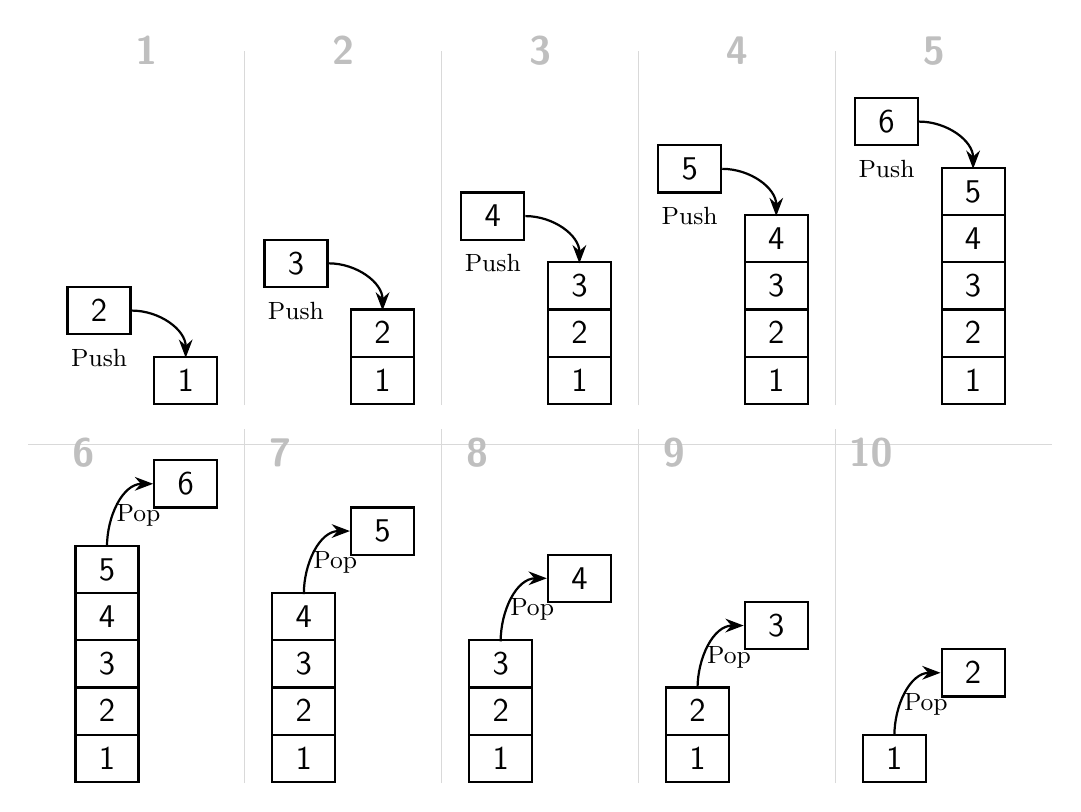
\begin{tikzpicture}[
				box/.style={draw, thick, minimum width=0.8cm, minimum height=0.6cm, anchor=south, font=\sffamily\large},
				lbl/.style={text=gray!50, font=\sffamily\Large\bfseries},
				arr/.style={->, >=Stealth, thick},
				val/.style={draw, thick, minimum width=0.8cm, minimum height=0.6cm, font=\sffamily\large}
				]
				
				% ==========================================
				% HÀNG 1: PUSH (Giữ nguyên như code trước - Đã chuẩn)
				% ==========================================
				
				% -- Cột 1 (Push 2 vào 1) --
				\begin{scope}[xshift=0cm]
					\node[lbl] at (0, 4.5) {1};
					\node[box] at (0.5,0) {1}; 
					\node[val] (val2) at (-0.6, 1.2) {2}; 
					\node[below=0.05cm of val2, font=\small] {Push};
					\draw[arr] (val2.east) to[out=0, in=90] (0.5, 0.6);
				\end{scope}
				
				% -- Cột 2 (Push 3) --
				\begin{scope}[xshift=2.5cm]
					\node[lbl] at (0, 4.5) {2};
					\draw[gray!30] (-1.25, 0) -- (-1.25, 4.5);
					\node[box] at (0.5,0) {1};
					\node[box] at (0.5,0.6) {2};
					\node[val] (val3) at (-0.6, 1.8) {3};
					\node[below=0.05cm of val3, font=\small] {Push};
					\draw[arr] (val3.east) to[out=0, in=90] (0.5, 1.2);
				\end{scope}
				
				% -- Cột 3 (Push 4) --
				\begin{scope}[xshift=5cm]
					\node[lbl] at (0, 4.5) {3};
					\draw[gray!30] (-1.25, 0) -- (-1.25, 4.5);
					\node[box] at (0.5,0) {1};
					\node[box] at (0.5,0.6) {2};
					\node[box] at (0.5,1.2) {3};
					\node[val] (val4) at (-0.6, 2.4) {4};
					\node[below=0.05cm of val4, font=\small] {Push};
					\draw[arr] (val4.east) to[out=0, in=90] (0.5, 1.8);
				\end{scope}
				
				% -- Cột 4 (Push 5) --
				\begin{scope}[xshift=7.5cm]
					\node[lbl] at (0, 4.5) {4};
					\draw[gray!30] (-1.25, 0) -- (-1.25, 4.5);
					\node[box] at (0.5,0) {1};
					\node[box] at (0.5,0.6) {2};
					\node[box] at (0.5,1.2) {3};
					\node[box] at (0.5,1.8) {4};
					\node[val] (val5) at (-0.6, 3.0) {5};
					\node[below=0.05cm of val5, font=\small] {Push};
					\draw[arr] (val5.east) to[out=0, in=90] (0.5, 2.4);
				\end{scope}
				
				% -- Cột 5 (Push 6) --
				\begin{scope}[xshift=10cm]
					\node[lbl] at (0, 4.5) {5};
					\draw[gray!30] (-1.25, 0) -- (-1.25, 4.5);
					\node[box] at (0.5,0) {1};
					\node[box] at (0.5,0.6) {2};
					\node[box] at (0.5,1.2) {3};
					\node[box] at (0.5,1.8) {4};
					\node[box] at (0.5,2.4) {5};
					\node[val] (val6) at (-0.6, 3.6) {6};
					\node[below=0.05cm of val6, font=\small] {Push};
					\draw[arr] (val6.east) to[out=0, in=90] (0.5, 3.0);
				\end{scope}
				
				
				% ==========================================
				% HÀNG 2: POP (ĐÃ CHỈNH SỬA: Dịch nội dung sang trái 0.5cm)
				% ==========================================
				% Logic thay đổi:
				% - Stack: x = -0.5 (cũ là 0)
				% - Giá trị Pop: x = 0.5 (cũ là 1.0)
				
				\draw[gray!30] (-1.5, -0.5) -- (11.5, -0.5); 
				
				% -- Cột 6 (Pop 6) --
				\begin{scope}[xshift=0cm, yshift=-4.8cm] 
					\node[lbl] at (-0.8, 4.2) {6};
					% Dịch stack sang -0.5
					\node[box] at (-0.5,0) {1};
					\node[box] at (-0.5,0.6) {2};
					\node[box] at (-0.5,1.2) {3};
					\node[box] at (-0.5,1.8) {4};
					\node[box] at (-0.5,2.4) {5};
					
					% Dịch hộp giá trị 6 sang 0.5
					\node[val] (pop6) at (0.5, 3.8) {6}; 
					
					% Chỉnh lại mũi tên và chữ
					\draw[arr] (-0.5, 3.0) to[out=90, in=180] (pop6.west);
					\node[font=\small] at (-0.1, 3.4) {Pop};
				\end{scope}
				
				% -- Cột 7 (Pop 5) --
				\begin{scope}[xshift=2.5cm, yshift=-4.8cm]
					\node[lbl] at (-0.8, 4.2) {7};
					\draw[gray!30] (-1.25, 0) -- (-1.25, 4.5);
					\node[box] at (-0.5,0) {1};
					\node[box] at (-0.5,0.6) {2};
					\node[box] at (-0.5,1.2) {3};
					\node[box] at (-0.5,1.8) {4};
					
					\node[val] (pop5) at (0.5, 3.2) {5};
					\draw[arr] (-0.5, 2.4) to[out=90, in=180] (pop5.west);
					\node[font=\small] at (-0.1, 2.8) {Pop};
				\end{scope}
				
				% -- Cột 8 (Pop 4) --
				\begin{scope}[xshift=5cm, yshift=-4.8cm]
					\node[lbl] at (-0.8, 4.2) {8};
					\draw[gray!30] (-1.25, 0) -- (-1.25, 4.5);
					\node[box] at (-0.5,0) {1};
					\node[box] at (-0.5,0.6) {2};
					\node[box] at (-0.5,1.2) {3};
					
					\node[val] (pop4) at (0.5, 2.6) {4};
					\draw[arr] (-0.5, 1.8) to[out=90, in=180] (pop4.west);
					\node[font=\small] at (-0.1, 2.2) {Pop};
				\end{scope}
				
				% -- Cột 9 (Pop 3) --
				\begin{scope}[xshift=7.5cm, yshift=-4.8cm]
					\node[lbl] at (-0.8, 4.2) {9};
					\draw[gray!30] (-1.25, 0) -- (-1.25, 4.5);
					\node[box] at (-0.5,0) {1};
					\node[box] at (-0.5,0.6) {2};
					
					\node[val] (pop3) at (0.5, 2.0) {3};
					\draw[arr] (-0.5, 1.2) to[out=90, in=180] (pop3.west);
					\node[font=\small] at (-0.1, 1.6) {Pop};
				\end{scope}
				
				% -- Cột 10 (Pop 2) --
				\begin{scope}[xshift=10cm, yshift=-4.8cm]
					\node[lbl] at (-0.8, 4.2) {10};
					\draw[gray!30] (-1.25, 0) -- (-1.25, 4.5);
					\node[box] at (-0.5,0) {1};
					
					\node[val] (pop2) at (0.5, 1.4) {2};
					\draw[arr] (-0.5, 0.6) to[out=90, in=180] (pop2.west);
					\node[font=\small] at (-0.1, 1.0) {Pop};
				\end{scope}
				
			\end{tikzpicture}
		\end{adjustbox}

		\begin{center}
			\footnotesize\textit{Nguồn: }\textcolor{blue}{\url{https://en.wikipedia.org/wiki/Stack_(abstract_data_type)}}
		\end{center}
	\end{frame}
	
	\begin{frame}[t,fragile]{Cài đặt ngăn xếp sử dụng danh sách liên kết đơn}
		\setlength{\leftmargini}{-1.2em}
		\small
		\begin{itemize}
			\item Cấu trúc và hàm khởi tạo thành phần
		\end{itemize}
		
		\vspace{0.15cm}
		
		\begin{tikzpicture}[remember picture]
			% --- Code box (left) ---
			\node (codebox) [anchor=north west, inner sep=0pt] at (0,0) {%
				\begin{tcolorbox}[
					width=0.62\textwidth,
					height=0.60\textheight,
					colback=white,
					colframe=black,
					boxrule=0.6pt,
					arc=0pt,
					left=-3pt,right=6pt,top=6pt,bottom=6pt
					]
					\begin{minted}[fontsize=\small, breaklines, linenos=false]{c}
						typedef struct Node{
							char value;
							struct Node* next;
						}Node;
						
						Node* makeNode(char v){
							Node* p = (Node*)malloc(sizeof(Node));
							p->value = v;
							p->next = NULL;
							return p;
						}
					\end{minted}
				\end{tcolorbox}
			};
			
			% --- Callout boxes (right) ---
			\node (note1) [draw, rectangle, thick, align=center, font=\large,
			minimum width=0.30\textwidth, minimum height=1.55cm,
			anchor=west]
			at ($(codebox.north east)+(0.9cm,-1.55cm)$)
			{Khai báo struct cho một\\phần tử của ngăn xếp};
			
			\node (note2) [draw, rectangle, thick, align=center, font=\large,
			minimum width=0.30\textwidth, minimum height=1.55cm,
			anchor=west]
			at ($(codebox.north east)+(0.9cm,-4.35cm)$)
			{Tạo một phần tử (node)\\của ngăn xếp};
			
			% ====== ARROWS (mũi tên ĐƠN, thẳng, không lệch) ======
			\tikzset{myarr/.style={->,>=Stealth,line width=0.85pt,shorten <=2pt,shorten >=2pt}}
			
			% target points = giao của (codebox.east) với cao độ của note (đảm bảo nằm đúng hàng)
			\coordinate (T1) at (codebox.east |- note1.west);
			\coordinate (T2) at (codebox.east |- note2.west);
			
			% vẽ mũi tên từ note sang code (đầu mũi tên ở phía code)
			\draw[myarr] (note1.west) -- (T1);
			\draw[myarr] (note2.west) -- (T2);
			
		\end{tikzpicture}
	\end{frame}
	
	\begin{frame}[t,fragile]{Cài đặt ngăn xếp sử dụng danh sách liên kết đơn}
		\setlength{\leftmargini}{-1.2em}
		\small
		\begin{itemize}
			\item Thao tác Push
		\end{itemize}
		
		\vspace{0.15cm}
		
		\begin{tikzpicture}[remember picture]
			% --- Code box (left) ---
			\node (codebox) [anchor=north west, inner sep=0pt] at (0,0) {%
				\begin{tcolorbox}[
					width=0.62\textwidth,
					height=0.60\textheight,
					colback=white,
					colframe=black,
					boxrule=0.6pt,
					arc=0pt,
					left=6pt,right=6pt,top=6pt,bottom=6pt
					]
					\begin{minted}[fontsize=\scriptsize, breaklines, linenos=false, escapeinside=|]{c}
						Node* push(Node* head, char v){
							Node* new_node = makeNode(v);|\tikz[remember picture,overlay]\node[inner sep=0pt,outer sep=0pt] (mkMake) {};|
							
							if(head == NULL) return new_node;|\tikz[remember picture,overlay]\node[inner sep=0pt,outer sep=0pt] (mkRet) {};|
							
							else{
								|\tikz[remember picture,overlay]\node[inner sep=0pt,outer sep=0pt] (blkTL) {};|new_node->next = head;|\tikz[remember picture,overlay]\node[inner sep=0pt,outer sep=0pt] (mkElse) {};|
								head = new_node;
								return head;|\tikz[remember picture,overlay]\node[inner sep=0pt,outer sep=0pt] (blkBR) {};|
							}
						}
					\end{minted}
				\end{tcolorbox}
			};
			
			% --- Callout boxes (right) ---
			\node (note1) [draw, rectangle, thick, align=center, font=\scriptsize,
			minimum width=0.30\textwidth, minimum height=0.90cm,
			anchor=west]
			at ($(codebox.north east)+(0.95cm,-1.15cm)$)
			{Tạo một node mới};
			
			\node (note2) [draw, rectangle, thick, align=center, font=\scriptsize,
			minimum width=0.30\textwidth, minimum height=1.20cm,
			anchor=west]
			at ($(codebox.north east)+(0.95cm,-2.75cm)$)
			{Nếu ngăn xếp rỗng, trả về phần\\tử mới tạo};
			
			\node (note3) [draw, rectangle, thick, align=center, font=\scriptsize,
			minimum width=0.30\textwidth, minimum height=1.80cm,
			anchor=west]
			at ($(codebox.north east)+(0.95cm,-4.65cm)$)
			{Nếu ngăn xếp không rỗng, biến\\node mới tạo thành phần tử\\đầu danh sách};
			
			% ====== GREEN HIGHLIGHT BOX (fit đúng khối else) ======
			% \coordinate (gTL) at ([xshift=-12pt,yshift=10pt]blkTL); 
			% \coordinate (gBR) at ([xshift=40pt,yshift=-4pt]blkBR); 
			% \draw[green!60!black, line width=1.0pt] (gTL) rectangle (gBR);
			
	% 		% ====== ARROWS: luôn dính đúng NOTE và trỏ đúng DÒNG CODE ======
	% 		\tikzset{myarr/.style={-Stealth, line width=0.85pt}};
			
	% 		% đích (tự chỉnh xshift/yshift nếu cần)
	% 		\coordinate (tMake) at ([xshift=-6pt,yshift=0pt]mkMake);
	% 		\coordinate (tRet)  at ([xshift=-6pt,yshift=0pt]mkRet);
	% 		\coordinate (tElse) at ([xshift=-6pt,yshift=0pt]mkElse);
			
	% 		% vẽ: xuất phát đúng note (không dùng |- nữa)
	% 		\draw[myarr] (note1.west) to[out=180,in=0,looseness=1.15] (tMake);
	% 		\draw[myarr] (note2.west) to[out=180,in=0,looseness=1.15] (tRet);
	% 		\draw[myarr] (note3.west) to[out=180,in=0,looseness=1.15] (tElse);
			
		\end{tikzpicture}
		
	\end{frame}
	
	% \begin{frame}[t,fragile]{Cài đặt ngăn xếp sử dụng danh sách liên kết đơn}
	% 	\setlength{\leftmargini}{-1.2em}
	% 	\small
	% 	\begin{itemize}
	% 		\item Thao tác Pop
	% 	\end{itemize}
		
	% 	\vspace{0.15cm}
		
	% 	\begin{tikzpicture}[remember picture]
	% 		% --- Code box (left) ---
	% 		\node (codebox) [anchor=north west, inner sep=0pt] at (0,0) {%
	% 			\begin{tcolorbox}[
	% 				width=0.62\textwidth,
	% 				height=0.60\textheight,
	% 				colback=white,
	% 				colframe=black,
	% 				boxrule=0.6pt,
	% 				arc=0pt,
	% 				left=6pt,right=6pt,top=6pt,bottom=6pt
	% 				]
	% 				\begin{minted}[fontsize=\large, breaklines, linenos=false, escapeinside=||]{c}
	% 					Node* pop(Node* head){
	% 						if(head == NULL) return head;|\tikz[remember picture,overlay]\node[inner sep=0pt,outer sep=0pt] (pEmptyRet) {};|
							
	% 						|\tikz[remember picture,overlay]\node[inner sep=0pt,outer sep=0pt] (blkTL) {};|Node* p = head;
	% 						head = head->next;
	% 						free(p);
	% 						return head;|\tikz[remember picture,overlay]\node[inner sep=0pt,outer sep=0pt] (blkBR) {};|
	% 					}
	% 				\end{minted}
	% 			\end{tcolorbox}
	% 		};
			
	% 		% ====== GREEN HIGHLIGHT BOX (nới ngang để bao hết) ======
	% 		\coordinate (gTL) at ([xshift=-12pt,yshift=10pt]blkTL);
	% 		\coordinate (gBR) at ([xshift=40pt,yshift=-4pt]blkBR);
	% 		\draw[green!60!black, line width=1.0pt] (gTL) rectangle (gBR);
			
	% 		% điểm giữa cạnh phải khung xanh (để cắm mũi tên 2)
	% 		\coordinate (gMid)   at ($(gTL)!0.5!(gBR)$);
	% 		\coordinate (gRight) at ($(gBR |- gMid)$);
			
	% 		% --- Callout boxes (right) ---
	% 		% ĐẶT NOTE THEO ĐÚNG CAO ĐỘ CỦA DÒNG CODE (để mũi tên luôn ngang & dính đúng khung)
	% 		\node (note1) [draw, rectangle, thick, align=center, font=\scriptsize,
	% 		minimum width=0.30\textwidth, minimum height=1.05cm,
	% 		anchor=west, outer sep=0pt]
	% 		at ($(codebox.east |- pEmptyRet)+(0.95cm,0)$)
	% 		{Nếu ngăn xếp rỗng, trả về rỗng};
			
	% 		\node (note2) [draw, rectangle, thick, align=center, font=\scriptsize,
	% 		minimum width=0.30\textwidth, minimum height=2.05cm,
	% 		anchor=west, outer sep=0pt]
	% 		at ($(codebox.east |- gRight)+(0.95cm,0)$)
	% 		{Nếu ngăn xếp không rỗng, xóa phần\\tử đầu của ngăn xếp và trả về phần\\tử đầu của ngăn xếp};
			
	% 		% ====== ARROWS: NOTE -> CODE (đuôi dính mép note, đầu ở code) ======
	% 		\tikzset{myarr/.style={-Stealth, line width=0.85pt}}
			
	% 		% nhích nhẹ mục tiêu về bên trái để đầu mũi tên không chạm chữ
	% 		\draw[myarr] (note1.west) -- ([xshift=-1pt]pEmptyRet);
	% 		\draw[myarr] (note2.west) -- (gRight);
			
	% 	\end{tikzpicture}
	% \end{frame}
	
	%================== SLIDE 10 ==================%
	\begin{frame}[t,fragile]{Cài đặt ngăn xếp sử dụng danh sách liên kết đơn}
		\setlength{\leftmargini}{-1.2em}
		\small
		\begin{itemize}
			\item Thao tác Top và isEmpty
		\end{itemize}
		
		\vspace{0.25cm}
		\begin{center}
			\begin{tcolorbox}[
				width=0.62\textwidth,
				colback=white,
				colframe=black,
				boxrule=0.6pt,
				arc=0pt,
				left=10pt,right=10pt,top=10pt,bottom=10pt
				]
				\begin{minted}[fontsize=\scriptsize, breaklines, linenos=false]{c}
					char top(Node* head){
						return head->value;
					}
					
					bool isEmpty(Node* head){
						if(head == NULL) return true;
						
						return false;
					}
				\end{minted}
			\end{tcolorbox}
		\end{center}
	\end{frame}
	
	
	%================== SLIDE 11 ==================%
	\begin{frame}[t]{Một số ứng dụng ngăn xếp}
		\setlength{\leftmargini}{-1.2em}
		\small
		
		\begin{itemize}
			\item \textbf{Ngăn xếp lời gọi hàm:} Ngăn xếp được sử dụng rộng rãi để quản lý cuộc gọi hàm và biến cục bộ trong ngôn ngữ lập trình. Khi một hàm được gọi, ngữ cảnh của nó (bao gồm đối số và biến cục bộ) được đẩy vào ngăn xếp. Khi hàm trả về, ngữ cảnh của nó được đẩy ra khỏi ngăn xếp, cho phép lồng ghép hàm một cách chính xác.
			\vspace{0.55cm}
			\item \textbf{Cơ chế quay lại (Undo):} Ngăn xếp được sử dụng trong các ứng dụng yêu cầu tính năng Hoàn tác, như trình soạn thảo văn bản, phần mềm đồ họa hoặc hệ thống quản lý phiên bản. Mỗi hành động của người dùng có thể được đẩy vào ngăn xếp, và việc hoàn tác một hành động liên quan đến việc lấy nó ra khỏi ngăn xếp để hoàn ngược thay đổi.
		\end{itemize}
	\end{frame}
	
	
	%================== SLIDE 12 ==================%
	\begin{frame}[t]{Một số ứng dụng ngăn xếp}
		\setlength{\leftmargini}{-1.2em}
		\small
		
		\begin{itemize}
			\item \textbf{Thuật toán Backtracking:} Trong các thuật toán như tìm kiếm theo chiều sâu (DFS) và các thuật toán backtracking (\textbf{Ví dụ:} giải quyết các câu đố như vấn đề N-Queens hoặc Sudoku), một ngăn xếp có thể được sử dụng để theo dõi các nút hoặc trạng thái đã được thăm. Điều này cho phép dễ dàng quay lại để khám phá các lựa chọn thay thế khi cần.
			\vspace{0.75cm}
			\item \textbf{Phân tích Biểu thức:} Ngăn xếp được sử dụng để phân tích và hiểu biểu thức trong các trình biên dịch và trình thông dịch. Chúng giúp duy trì thứ tự ưu tiên của các toán tử và đánh giá biểu thức một cách chính xác.
		\end{itemize}
	\end{frame}
	
	
	%================== SLIDE 13 ==================%
	\begin{frame}[t]{Một số ứng dụng ngăn xếp}
		\setlength{\leftmargini}{-1.2em}
		\small
		
		\begin{itemize}
			\item \textbf{Quản lý Bộ nhớ:} Ngăn xếp đóng vai trò quan trọng trong quản lý bộ nhớ trong các hệ thống máy tính. Chúng được sử dụng để quản lý ngăn xếp gọi hàm, nơi lưu trữ thông tin về cuộc gọi hàm và biến cục bộ. Ngăn xếp giúp phân bổ bộ nhớ cho cuộc gọi hàm và giải phóng nó khi các hàm trả về, ngăn chặn rò rỉ bộ nhớ.
			\vspace{0.80cm}
			\item \textbf{Phân tích Biểu thức:} Ngăn xếp được sử dụng để phân tích và hiểu biểu thức trong các trình biên dịch và trình thông dịch. Chúng giúp duy trì thứ tự ưu tiên của các toán tử và đánh giá biểu thức một cách chính xác.
		\end{itemize}
	\end{frame}
	
	\section{Bài tập: Kiểm tra tính cân xứng của dãy ngoặc}
	
	\begin{frame}{Bài toán kiểm tra tính cân xứng của dãy ngoặc}
	\setlength{\leftmargini}{-1.2em}
		
		\begin{itemize}
			\item Cho dãy dấu ngoặc $E$ mà mỗi phần tử là một dấu ngoặc thuộc một trong các loại: $(, ), [, ], \{, \}$. Viết chương trình kiểm tra xem dãy ngoặc đó có cân xứng (balanced) hay không?
			
			\item Ví dụ:
			\begin{itemize}
				\item \texttt{()[\{\}([])]}: cân xứng
				\item \texttt{()[\{\}([]\}]}: không cân xứng
			\end{itemize}
		\end{itemize}
	\end{frame}
	
	\begin{frame}{Bài toán kiểm tra tính cân xứng của dãy ngoặc}
		\setlength{\leftmargini}{-1.2em}
		\begin{columns}[T]
			
			% --- Cột trái: Văn bản mô tả ---
			\begin{column}{0.58\textwidth}
				\setlength{\leftmargini}{1.2em}
				\begin{itemize}
					\setlength{\itemsep}{2.5em}
					
					\item Dữ liệu đầu vào:
					\begin{itemize}
						\item Một dòng duy nhất chứa xâu ký tự thể hiện dãy dấu ngoặc
					\end{itemize}
					
					\item Kết quả đầu ra:
					\begin{itemize}
						\item Ghi 1 nếu dãy dấu ngoặc là cân xứng và ghi 0, nếu dãy dấu ngoặc không cân xứng
					\end{itemize}
				\end{itemize}
			\end{column}
			
			% --- Cột phải: Bảng ví dụ (Đã redesign giống hình) ---
			\begin{column}{0.40\textwidth}
				\vspace{0.5cm} % Căn lề trên
				
				% Thiết lập dãn dòng cho bảng rộng rãi giống hình
				\renewcommand{\arraystretch}{1.5} 
				
				% --- Bảng 1 ---
				% p{...} để cố định chiều rộng cột, | để tạo đường kẻ dọc
				\begin{tabular}{|p{3.8cm}|p{1.5cm}|}
					\hline
					% \multicolumn để gộp ô và căn giữa tiêu đề
					\multicolumn{1}{|c|}{\textbf{stdin}} & \multicolumn{1}{c|}{\textbf{stdout}} \\
					\hline
					\textcolor{codeblue}{\texttt{()[\{\}([])]}} & 1 \\
					\hline
				\end{tabular}
				
				\vspace{1.5cm} % Khoảng cách giữa 2 bảng
				
				% --- Bảng 2 ---
				\begin{tabular}{|p{3.8cm}|p{1.5cm}|}
					\hline
					\multicolumn{1}{|c|}{\textbf{stdin}} & \multicolumn{1}{c|}{\textbf{stdout}} \\
					\hline
					\textcolor{codeblue}{\texttt{()[\{\}([]\}]}} & 0 \\
					\hline
				\end{tabular}
				
			\end{column}
		\end{columns}
	\end{frame}
	
	\begin{frame}[t]{Bài toán kiểm tra tính cân xứng của dãy ngoặc}
		\setlength{\leftmargini}{-1.2em}
		
		\begin{itemize}
			\item \textbf{Thuật toán}
		\end{itemize}
		\begin{enumerate}
			\item Khởi tạo một ngăn xếp rỗng $S$.
			\item Duyệt dãy dấu ngoặc từ trái qua phải:
			\begin{itemize}
				\item Nếu gặp ngoặc mở $A$ thì đưa ngoặc mở đó vào $S$.
				\item Nếu gặp ngoặc đóng $B$:
				
				\hspace{0.6cm}-- Nếu $S$ rỗng $\Rightarrow$ kết luận dãy ngoặc $E$ không cân xứng.
				
				\hspace{0.6cm}-- Nếu $S$ không rỗng: lấy một ngoặc mở $A$ khỏi $S$; nếu $A$ và $B$ không cân xứng (khác loại) $\Rightarrow$ kết luận $E$ không cân xứng.
			\end{itemize}
			\item Kết thúc duyệt: nếu $S$ không rỗng thì $E$ không cân xứng; ngược lại thì $E$ là cân xứng.
		\end{enumerate}
	\end{frame}
	
	%======================
	% Minh hoạ số 1: ( ) [ ( { { } } ) ]
	% Slide 18 -> 22
	%======================
	
	% --- Slide 18: Khởi tạo ---
	\begin{frame}[t]{Minh hoạ}
		\setlength{\leftmargini}{-1.2em}
		\small
		
		\begin{columns}[T,onlytextwidth]
			\column{0.72\textwidth}
			\begin{itemize}
				\item \textbf{Minh hoạ số 1: dãy ngoặc \texttt{( ) [ ( \{ \{ \} \} ) ]}}
				\begin{itemize}
					\item Khởi tạo ngăn xếp rỗng, thực hiện duyệt dãy ngoặc từ trái qua phải
				\end{itemize}
			\end{itemize}
			
			\column{0.28\textwidth}
			\vspace{0.55cm}
			\begin{flushright}
				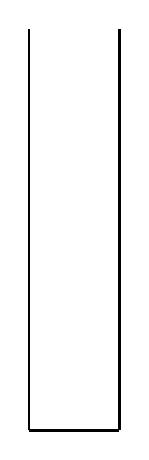
\begin{tikzpicture}[x=1cm,y=1cm]
					\def\W{1.15}
					\def\H{5.10}
					\draw[line width=0.9pt] (0,0) -- (0,\H);
					\draw[line width=0.9pt] (\W,0) -- (\W,\H);
					\draw[line width=0.9pt] (0,0) -- (\W,0);
				\end{tikzpicture}
			\end{flushright}
		\end{columns}
	\end{frame}
	
	% --- Slide 19: Bước 1 (push '(') ---
	\begin{frame}[t]{Minh hoạ}
		\setlength{\leftmargini}{-1.2em}
		\small
		
		\begin{columns}[T,onlytextwidth]
			\column{0.72\textwidth}
			\begin{itemize}
				\item \textbf{Minh hoạ số 1: dãy ngoặc \texttt{( ) [ ( \{ \{ \} \} ) ]}}
				\begin{itemize}
					\item Bước 1: Xét ngoặc tiếp theo là ngoặc mở ``('' $\rightarrow$ đưa ngoặc mở vào ngăn xếp
				\end{itemize}
			\end{itemize}
			
			\column{0.28\textwidth}
			\vspace{0.55cm}
			\begin{flushright}
				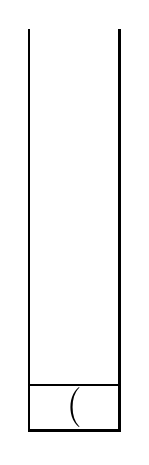
\begin{tikzpicture}[x=1cm,y=1cm]
					\def\W{1.15}
					\def\H{5.10}
					\def\cell{0.58}
					
					\draw[line width=0.9pt] (0,0) -- (0,\H);
					\draw[line width=0.9pt] (\W,0) -- (\W,\H);
					\draw[line width=0.9pt] (0,0) -- (\W,0);
					
					\draw[line width=0.9pt] (0,0) rectangle (\W,\cell);
					\node[font=\Large] at (\W/2,0.5*\cell) {(};
				\end{tikzpicture}
			\end{flushright}
		\end{columns}
	\end{frame}
	
	% --- Slide 20: Bước 1 + Bước 2 (như ảnh) ---
	\begin{frame}[t]{Minh hoạ}
		\setlength{\leftmargini}{-1.2em}
		\small
		
		\begin{columns}[T,onlytextwidth]
			\column{0.72\textwidth}
			\begin{itemize}
				\item \textbf{Minh hoạ số 1: dãy ngoặc \texttt{( ) [ ( \{ \{ \} \} ) ]}}
				\begin{itemize}
					\item Bước 1: Xét ngoặc tiếp theo là ngoặc mở ``('' $\rightarrow$ đưa ngoặc mở vào ngăn xếp
					\item Bước 2: Xét ngoặc tiếp theo là ngoặc đóng ``)'' $\rightarrow$ lấy ngoặc mở ra khỏi ngăn\\
					xếp và so khớp ``('' ``)'' $\rightarrow$ kết quả là đúng nên ta tiếp tục duyệt
				\end{itemize}
			\end{itemize}
			
			\column{0.28\textwidth}
			\vspace{0.55cm}
			\begin{flushright}
				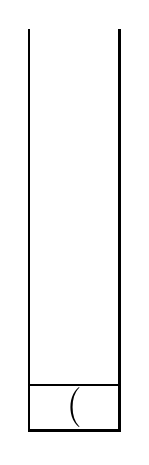
\begin{tikzpicture}[x=1cm,y=1cm]
					\def\W{1.15}
					\def\H{5.10}
					\def\cell{0.58}
					
					\draw[line width=0.9pt] (0,0) -- (0,\H);
					\draw[line width=0.9pt] (\W,0) -- (\W,\H);
					\draw[line width=0.9pt] (0,0) -- (\W,0);
					
					% (giữ như ảnh bạn gửi: vẫn hiển thị '(' ở đáy)
					\draw[line width=0.9pt] (0,0) rectangle (\W,\cell);
					\node[font=\Large] at (\W/2,0.5*\cell) {(};
				\end{tikzpicture}
			\end{flushright}
		\end{columns}
	\end{frame}
	
	% --- Slide 21: Bước 3 (push '[') ---
	\begin{frame}[t]{Minh hoạ}
		\setlength{\leftmargini}{-1.2em}
		\small
		
		\begin{columns}[T,onlytextwidth]
			\column{0.72\textwidth}
			\begin{itemize}
				\item \textbf{Minh hoạ số 1: dãy ngoặc \texttt{( ) [ ( \{ \{ \} \} ) ]}}
				\begin{itemize}
					\item Bước 1: Xét ngoặc tiếp theo là ngoặc mở ``('' $\rightarrow$ đưa ngoặc mở vào ngăn xếp
					\item Bước 2: Xét ngoặc tiếp theo là ngoặc đóng ``)'' $\rightarrow$ lấy ngoặc mở ra khỏi ngăn\\
					xếp và so khớp ``('' ``)'' $\rightarrow$ kết quả là đúng nên ta tiếp tục duyệt
					\item Bước 3: Gặp ngoặc mở ``['' $\rightarrow$ đưa ngoặc mở này vào ngăn xếp
				\end{itemize}
			\end{itemize}
			
			\column{0.28\textwidth}
			\vspace{0.55cm}
			\begin{flushright}
				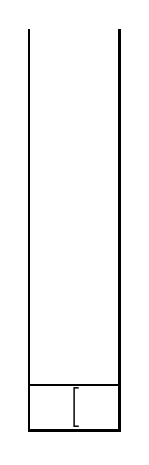
\begin{tikzpicture}[x=1cm,y=1cm]
					\def\W{1.15}
					\def\H{5.10}
					\def\cell{0.58}
					
					\draw[line width=0.9pt] (0,0) -- (0,\H);
					\draw[line width=0.9pt] (\W,0) -- (\W,\H);
					\draw[line width=0.9pt] (0,0) -- (\W,0);
					
					\draw[line width=0.9pt] (0,0) rectangle (\W,\cell);
					\node[font=\Large] at (\W/2,0.5*\cell) {[};
				\end{tikzpicture}
			\end{flushright}
		\end{columns}
	\end{frame}
	
	% --- Slide 22: Bước 4 (push '(' lên trên '[') ---
	\begin{frame}[t]{Minh hoạ}
		\setlength{\leftmargini}{-1.2em}
		\small
		
		\begin{columns}[T,onlytextwidth]
			\column{0.72\textwidth}
			\begin{itemize}
				\item \textbf{Minh hoạ số 1: dãy ngoặc \texttt{( ) [ ( \{ \{ \} \} ) ]}}
				\begin{itemize}
					\item Bước 1: Xét ngoặc tiếp theo là ngoặc mở ``('' $\rightarrow$ đưa ngoặc mở vào ngăn xếp
					\item Bước 2: Xét ngoặc tiếp theo là ngoặc đóng ``)'' $\rightarrow$ lấy ngoặc mở ra khỏi ngăn\\
					xếp và so khớp ``('' ``)'' $\rightarrow$ kết quả là đúng nên ta tiếp tục duyệt
					\item Bước 3: Gặp ngoặc mở ``['' $\rightarrow$ đưa ngoặc mở này vào ngăn xếp
					\item Bước 4: Gặp ngoặc mở ``('' $\rightarrow$ đưa ngoặc mở này vào ngăn xếp
				\end{itemize}
			\end{itemize}
			
			\column{0.28\textwidth}
			\vspace{0.55cm}
			\begin{flushright}
				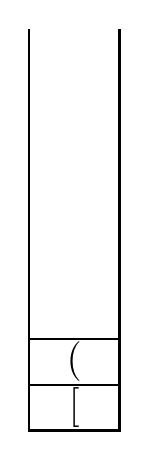
\begin{tikzpicture}[x=1cm,y=1cm]
					\def\W{1.15}
					\def\H{5.10}
					\def\cell{0.58}
					
					\draw[line width=0.9pt] (0,0) -- (0,\H);
					\draw[line width=0.9pt] (\W,0) -- (\W,\H);
					\draw[line width=0.9pt] (0,0) -- (\W,0);
					
					% bottom: '['
					\draw[line width=0.9pt] (0,0) rectangle (\W,\cell);
					\node[font=\Large] at (\W/2,0.5*\cell) {[};
					% top: '('
					\draw[line width=0.9pt] (0,\cell) rectangle (\W,2*\cell);
					\node[font=\Large] at (\W/2,1.5*\cell) {(};
				\end{tikzpicture}
			\end{flushright}
		\end{columns}
	\end{frame}
	
	%========================
	% SLIDE 23
	%========================
	\begin{frame}[t]{Minh hoạ}
		\setlength{\leftmargini}{-1.2em}
		\small
		
		\begin{columns}[T,onlytextwidth]
			\column{0.72\textwidth}
			\begin{itemize}
				\item \textbf{Minh hoạ số 1: dãy ngoặc \texttt{()[(\{\})]}}
				\begin{itemize}
					\item Bước 1: Xét ngoặc tiếp theo là ngoặc mở ``('' $\rightarrow$ đưa ngoặc mở vào ngăn\\
					xếp
					\item Bước 2: Xét ngoặc tiếp theo là ngoặc đóng ``)'' $\rightarrow$ lấy ngoặc mở ra khỏi\\
					ngăn xếp và so khớp ``('' ``)'' $\rightarrow$ kết quả là đúng nên ta tiếp tục duyệt
					\item Bước 3: Gặp ngoặc mở ``['' $\rightarrow$ đưa ngoặc mở này vào ngăn xếp
					\item Bước 4: Gặp ngoặc mở ``('' $\rightarrow$ đưa ngoặc mở này vào ngăn xếp
					\item Bước 5: Gặp ngoặc mở ``\{'' $\rightarrow$ đưa ngoặc mở này vào ngăn xếp
				\end{itemize}
			\end{itemize}
			
			\column{0.28\textwidth}
			\vspace{0.55cm}
			\begin{flushright}
				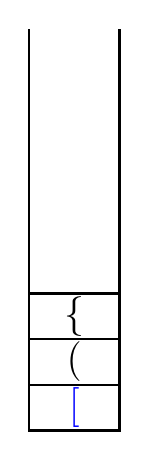
\begin{tikzpicture}[x=1cm,y=1cm]
					\def\W{1.15}
					\def\H{5.10}
					\def\cell{0.58}
					\draw[line width=0.9pt] (0,0) -- (0,\H);
					\draw[line width=0.9pt] (\W,0) -- (\W,\H);
					\draw[line width=0.9pt] (0,0) -- (\W,0);
					
					% bottom: [
					\draw[line width=0.9pt] (0,0) rectangle (\W,\cell);
					\node[font=\Large] at (\W/2,0.5*\cell) {\textcolor{blue}{[}};
					% middle: (
					\draw[line width=0.9pt] (0,\cell) rectangle (\W,2*\cell);
					\node[font=\Large] at (\W/2,1.5*\cell) {(};
					% top: {
						\draw[line width=0.9pt] (0,2*\cell) rectangle (\W,3*\cell);
						\node[font=\Large] at (\W/2,2.5*\cell) {\{ };
					\end{tikzpicture}
				\end{flushright}
			\end{columns}
		\end{frame}
		
		
		%========================
		% SLIDE 24
		%========================
		\begin{frame}[t]{Minh hoạ}
			\setlength{\leftmargini}{-1.2em}
			\small
			
			\begin{columns}[T,onlytextwidth]
				\column{0.72\textwidth}
				\begin{itemize}
					\item \textbf{Minh hoạ số 1: dãy ngoặc \texttt{()[(\{\})]}}
					\begin{itemize}
						\item Bước 1: Xét ngoặc tiếp theo là ngoặc mở ``('' $\rightarrow$ đưa ngoặc mở vào ngăn\\
						xếp
						\item Bước 2: Xét ngoặc tiếp theo là ngoặc đóng ``)'' $\rightarrow$ lấy ngoặc mở ra khỏi\\
						ngăn xếp và so khớp ``('' ``)'' $\rightarrow$ kết quả là đúng nên ta tiếp tục duyệt
						\item Bước 3: Gặp ngoặc mở ``['' $\rightarrow$ đưa ngoặc mở này vào ngăn xếp
						\item Bước 4: Gặp ngoặc mở ``('' $\rightarrow$ đưa ngoặc mở này vào ngăn xếp
						\item Bước 5: Gặp ngoặc mở ``\{'' $\rightarrow$ đưa ngoặc mở này vào ngăn xếp
						\item Bước 6: Gặp ngoặc đóng ``\}'' $\rightarrow$ lấy 1 ngoặc mở là ``\{'' ra khỏi ngăn xếp
					\end{itemize}
				\end{itemize}
				
				\column{0.28\textwidth}
				\vspace{0.55cm}
				\begin{flushright}
					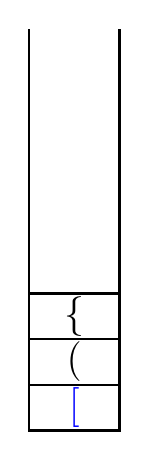
\begin{tikzpicture}[x=1cm,y=1cm]
						\def\W{1.15}
						\def\H{5.10}
						\def\cell{0.58}
						\draw[line width=0.9pt] (0,0) -- (0,\H);
						\draw[line width=0.9pt] (\W,0) -- (\W,\H);
						\draw[line width=0.9pt] (0,0) -- (\W,0);
						
						% bottom: [
						\draw[line width=0.9pt] (0,0) rectangle (\W,\cell);
						\node[font=\Large] at (\W/2,0.5*\cell) {\textcolor{blue}{[}};
						% middle: (
						\draw[line width=0.9pt] (0,\cell) rectangle (\W,2*\cell);
						\node[font=\Large] at (\W/2,1.5*\cell) {(};
						% top: {
							\draw[line width=0.9pt] (0,2*\cell) rectangle (\W,3*\cell);
							\node[font=\Large] at (\W/2,2.5*\cell) {\{ };
						\end{tikzpicture}
					\end{flushright}
				\end{columns}
			\end{frame}
			
			
			%========================
			% SLIDE 25
			%========================
			\begin{frame}[t]{Minh hoạ}
				\setlength{\leftmargini}{-1.2em}
				\small
				
				\begin{columns}[T,onlytextwidth]
					\column{0.72\textwidth}
					\begin{itemize}
						\item \textbf{Minh hoạ số 1: dãy ngoặc \texttt{()[(\{\})]}}
						\begin{itemize}
							\item Bước 5: Gặp ngoặc mở ``\{'' $\rightarrow$ đưa ngoặc mở này vào ngăn xếp
							\item Bước 6: Gặp ngoặc đóng ``\}'' $\rightarrow$ lấy 1 ngoặc mở là ``\{'' ra khỏi ngăn xếp
							\begin{itemize}
								\item So khớp ``\{'' ``\}'' $\rightarrow$ kết quả là đúng nên ta tiếp tục duyệt
							\end{itemize}
						\end{itemize}
					\end{itemize}
					
					\column{0.28\textwidth}
					\vspace{0.55cm}
					\begin{flushright}
						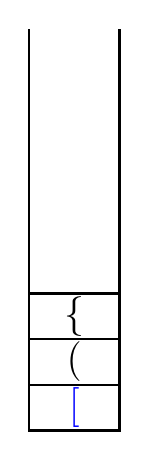
\begin{tikzpicture}[x=1cm,y=1cm]
							\def\W{1.15}
							\def\H{5.10}
							\def\cell{0.58}
							\draw[line width=0.9pt] (0,0) -- (0,\H);
							\draw[line width=0.9pt] (\W,0) -- (\W,\H);
							\draw[line width=0.9pt] (0,0) -- (\W,0);
							
							% bottom: [
							\draw[line width=0.9pt] (0,0) rectangle (\W,\cell);
							\node[font=\Large] at (\W/2,0.5*\cell) {\textcolor{blue}{[}};
							% middle: (
							\draw[line width=0.9pt] (0,\cell) rectangle (\W,2*\cell);
							\node[font=\Large] at (\W/2,1.5*\cell) {(};
							% top: {
								\draw[line width=0.9pt] (0,2*\cell) rectangle (\W,3*\cell);
								\node[font=\Large] at (\W/2,2.5*\cell) {\{ };
							\end{tikzpicture}
						\end{flushright}
					\end{columns}
				\end{frame}
				
				
				%========================
				% SLIDE 26
				%========================
				\begin{frame}[t]{Minh hoạ}
					\setlength{\leftmargini}{-1.2em}
					\small
					
					\begin{columns}[T,onlytextwidth]
						\column{0.72\textwidth}
						\begin{itemize}
							\item \textbf{Minh hoạ số 1: dãy ngoặc \texttt{()[(\{\})]}}
							\begin{itemize}
								\item Bước 5: Gặp ngoặc mở ``\{'' $\rightarrow$ đưa ngoặc mở này vào ngăn xếp
								\item Bước 6: Gặp ngoặc đóng ``\}'' $\rightarrow$ lấy 1 ngoặc mở là ``\{'' ra khỏi ngăn xếp
								\begin{itemize}
									\item So khớp ``\{'' ``\}'' $\rightarrow$ kết quả là đúng nên ta tiếp tục duyệt
								\end{itemize}
								\item Bước 7: Gặp ngoặc đóng ``)'' $\rightarrow$ lấy 1 ngoặc mở là ``('' ra khỏi ngăn xếp
							\end{itemize}
						\end{itemize}
						
						\column{0.28\textwidth}
						\vspace{0.55cm}
						\begin{flushright}
							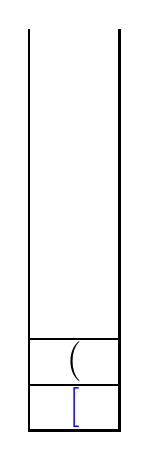
\begin{tikzpicture}[x=1cm,y=1cm]
								\def\W{1.15}
								\def\H{5.10}
								\def\cell{0.58}
								\draw[line width=0.9pt] (0,0) -- (0,\H);
								\draw[line width=0.9pt] (\W,0) -- (\W,\H);
								\draw[line width=0.9pt] (0,0) -- (\W,0);
								
								% bottom: [
								\draw[line width=0.9pt] (0,0) rectangle (\W,\cell);
								\node[font=\Large] at (\W/2,0.5*\cell) {\textcolor{blue}{[}};
								% top: (
								\draw[line width=0.9pt] (0,\cell) rectangle (\W,2*\cell);
								\node[font=\Large] at (\W/2,1.5*\cell) {(};
							\end{tikzpicture}
						\end{flushright}
					\end{columns}
				\end{frame}
				
				
				%========================
				% SLIDE 27
				%========================
				\begin{frame}[t]{Minh hoạ}
					\setlength{\leftmargini}{-1.2em}
					\small
					
					\begin{columns}[T,onlytextwidth]
						\column{0.72\textwidth}
						\begin{itemize}
							\item \textbf{Minh hoạ số 1: dãy ngoặc \texttt{()[(\{\})]}}
							\begin{itemize}
								\item Bước 5: Gặp ngoặc mở ``\{'' $\rightarrow$ đưa ngoặc mở này vào ngăn xếp
								\item Bước 6: Gặp ngoặc đóng ``\}'' $\rightarrow$ lấy 1 ngoặc mở là ``\{'' ra khỏi ngăn xếp
								\begin{itemize}
									\item So khớp ``\{'' ``\}'' $\rightarrow$ kết quả là đúng nên ta tiếp tục duyệt
								\end{itemize}
								\item Bước 7: Gặp ngoặc đóng ``)'' $\rightarrow$ lấy 1 ngoặc mở là ``('' ra khỏi ngăn xếp
								\begin{itemize}
									\item So khớp ``('' ``)'' $\rightarrow$ kết quả là đúng nên ta tiếp tục duyệt
								\end{itemize}
							\end{itemize}
						\end{itemize}
						
						\column{0.28\textwidth}
						\vspace{0.55cm}
						\begin{flushright}
							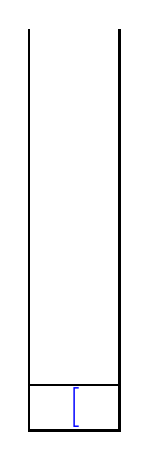
\begin{tikzpicture}[x=1cm,y=1cm]
								\def\W{1.15}
								\def\H{5.10}
								\def\cell{0.58}
								\draw[line width=0.9pt] (0,0) -- (0,\H);
								\draw[line width=0.9pt] (\W,0) -- (\W,\H);
								\draw[line width=0.9pt] (0,0) -- (\W,0);
								
								% bottom: [
								\draw[line width=0.9pt] (0,0) rectangle (\W,\cell);
								\node[font=\Large] at (\W/2,0.5*\cell) {\textcolor{blue}{[}};
							\end{tikzpicture}
						\end{flushright}
					\end{columns}
				\end{frame}
				
				
				%========================
				% SLIDE 28
				%========================
				\begin{frame}[t]{Minh hoạ}
					\setlength{\leftmargini}{-1.2em}
					\small
					
					\begin{columns}[T,onlytextwidth]
						\column{0.72\textwidth}
						\begin{itemize}
							\item \textbf{Minh hoạ số 1: dãy ngoặc \texttt{()[(\{\})]}}
							\begin{itemize}
								\item Bước 5: Gặp ngoặc mở ``\{'' $\rightarrow$ đưa ngoặc mở này vào ngăn xếp
								\item Bước 6: Gặp ngoặc đóng ``\}'' $\rightarrow$ lấy 1 ngoặc mở là ``\{'' ra khỏi ngăn xếp
								\begin{itemize}
									\item So khớp ``\{'' ``\}'' $\rightarrow$ kết quả là đúng nên ta tiếp tục duyệt
								\end{itemize}
								\item Bước 7: Gặp ngoặc đóng ``)'' $\rightarrow$ lấy 1 ngoặc mở là ``('' ra khỏi ngăn xếp
								\begin{itemize}
									\item So khớp ``('' ``)'' $\rightarrow$ kết quả là đúng nên ta tiếp tục duyệt
								\end{itemize}
								\item Bước 8: Gặp ngoặc đóng ``]'' $\rightarrow$ lấy 1 ngoặc mở là ``['' ra khỏi ngăn xếp
							\end{itemize}
						\end{itemize}
						
						\column{0.28\textwidth}
						\vspace{0.55cm}
						\begin{flushright}
							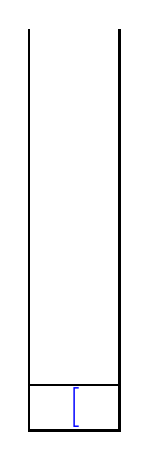
\begin{tikzpicture}[x=1cm,y=1cm]
								\def\W{1.15}
								\def\H{5.10}
								\def\cell{0.58}
								\draw[line width=0.9pt] (0,0) -- (0,\H);
								\draw[line width=0.9pt] (\W,0) -- (\W,\H);
								\draw[line width=0.9pt] (0,0) -- (\W,0);
								
								% bottom: [
								\draw[line width=0.9pt] (0,0) rectangle (\W,\cell);
								\node[font=\Large] at (\W/2,0.5*\cell) {\textcolor{blue}{[}};
							\end{tikzpicture}
						\end{flushright}
					\end{columns}
				\end{frame}
				
				
				%========================
				% SLIDE 29
				%========================
				\begin{frame}[t]{Minh hoạ}
					\setlength{\leftmargini}{-1.2em}
					\small
					
					\begin{columns}[T,onlytextwidth]
						\column{0.72\textwidth}
						\begin{itemize}
							\item \textbf{Minh hoạ số 1: dãy ngoặc \texttt{()[(\{\})]}}
							\begin{itemize}
								\item Bước 5: Gặp ngoặc mở ``\{'' $\rightarrow$ đưa ngoặc mở này vào ngăn xếp
								\item Bước 6: Gặp ngoặc đóng ``\}'' $\rightarrow$ lấy 1 ngoặc mở là ``\{'' ra khỏi ngăn xếp
								\begin{itemize}
									\item So khớp ``\{'' ``\}'' $\rightarrow$ kết quả là đúng nên ta tiếp tục duyệt
								\end{itemize}
								\item Bước 7: Gặp ngoặc đóng ``)'' $\rightarrow$ lấy 1 ngoặc mở là ``('' ra khỏi ngăn xếp
								\begin{itemize}
									\item So khớp ``('' ``)'' $\rightarrow$ kết quả là đúng nên ta tiếp tục duyệt
								\end{itemize}
								\item Bước 8: Gặp ngoặc đóng ``]'' $\rightarrow$ lấy 1 ngoặc mở là ``['' ra khỏi ngăn xếp
								\begin{itemize}
									\item So khớp ``['' ``]'' $\rightarrow$ lúc này dãy ngoặc đã duyệt xong và ngăn xếp rỗng,\\
									nên kết quả dãy ngoặc này là cân xứng
								\end{itemize}
							\end{itemize}
						\end{itemize}
						
						\column{0.28\textwidth}
						\vspace{0.55cm}
						\begin{flushright}
							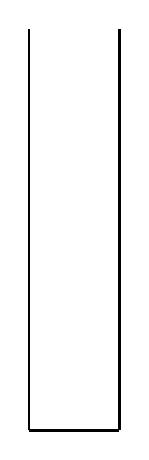
\begin{tikzpicture}[x=1cm,y=1cm]
								\def\W{1.15}
								\def\H{5.10}
								\def\cell{0.58}
								\draw[line width=0.9pt] (0,0) -- (0,\H);
								\draw[line width=0.9pt] (\W,0) -- (\W,\H);
								\draw[line width=0.9pt] (0,0) -- (\W,0);
								% stack rỗng
							\end{tikzpicture}
						\end{flushright}
					\end{columns}
				\end{frame}
				
				
				%========================
				% SLIDE 30 (Minh hoạ số 2 - khởi tạo)
				%========================
				\begin{frame}[t]{Minh hoạ}
					\setlength{\leftmargini}{-1.2em}
					\small
					
					\begin{columns}[T,onlytextwidth]
						\column{0.72\textwidth}
						\begin{itemize}
							\item \textbf{Minh hoạ số 2: dãy ngoặc \texttt{()[(\}\})]}}
							\begin{itemize}
								\item Khởi tạo ngăn xếp rỗng và duyệt dãy ngoặc từ trái qua phải
							\end{itemize}
						\end{itemize}
						
						\column{0.28\textwidth}
						\vspace{0.55cm}
						\begin{flushright}
							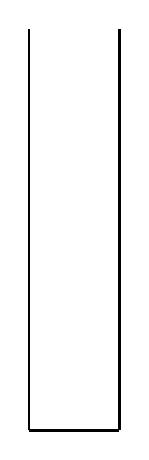
\begin{tikzpicture}[x=1cm,y=1cm]
								\def\W{1.15}
								\def\H{5.10}
								\draw[line width=0.9pt] (0,0) -- (0,\H);
								\draw[line width=0.9pt] (\W,0) -- (\W,\H);
								\draw[line width=0.9pt] (0,0) -- (\W,0);
							\end{tikzpicture}
						\end{flushright}
					\end{columns}
				\end{frame}
				
				%========================
				% SLIDE 31
				%========================
				\begin{frame}[t]{Lato}
					\setlength{\leftmargini}{-1.2em}
					\small
					
					\begin{columns}[T,onlytextwidth]
						\column{0.72\textwidth}
						\begin{itemize}
							\item \textbf{Minh hoạ số 2: dãy ngoặc \texttt{()[(\}\})]}}
							\begin{itemize}
								\item Bước 1: Gặp ngoặc tiếp theo là ngoặc mở ``('' $\rightarrow$ đưa ngoặc mở này\\
								vào ngăn xếp
							\end{itemize}
						\end{itemize}
						
						\column{0.28\textwidth}
						\vspace{0.55cm}
						\begin{flushright}
							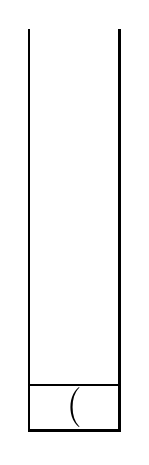
\begin{tikzpicture}[x=1cm,y=1cm]
								\def\W{1.15}
								\def\H{5.10}
								\def\cell{0.58}
								\draw[line width=0.9pt] (0,0) -- (0,\H);
								\draw[line width=0.9pt] (\W,0) -- (\W,\H);
								\draw[line width=0.9pt] (0,0) -- (\W,0);
								
								\draw[line width=0.9pt] (0,0) rectangle (\W,\cell);
								\node[font=\Large] at (\W/2,0.5*\cell) {(};
							\end{tikzpicture}
						\end{flushright}
					\end{columns}
				\end{frame}
				
				%========================
				% SLIDE 32
				%========================
				\begin{frame}[t]{Lato}
					\setlength{\leftmargini}{-1.2em}
					\small
					
					\begin{columns}[T,onlytextwidth]
						\column{0.72\textwidth}
						\begin{itemize}
							\item \textbf{Minh hoạ số 2: dãy ngoặc \texttt{()[(\}\})]}}
							\begin{itemize}
								\item Bước 1: Gặp ngoặc tiếp theo là ngoặc mở ``('' $\rightarrow$ đưa ngoặc mở này\\
								vào ngăn xếp
								\item Bước 2: Gặp ngoặc tiếp theo là ngoặc đóng ``)'' $\rightarrow$ lấy 1 ngoặc mở là\\
								``('' ra khỏi ngăn xếp
							\end{itemize}
						\end{itemize}
						
						\column{0.28\textwidth}
						\vspace{0.55cm}
						\begin{flushright}
							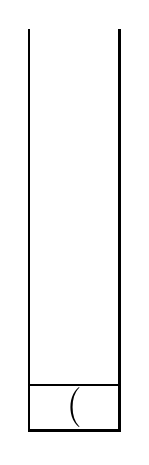
\begin{tikzpicture}[x=1cm,y=1cm]
								\def\W{1.15}
								\def\H{5.10}
								\def\cell{0.58}
								\draw[line width=0.9pt] (0,0) -- (0,\H);
								\draw[line width=0.9pt] (\W,0) -- (\W,\H);
								\draw[line width=0.9pt] (0,0) -- (\W,0);
								
								% (đúng như ảnh: vẫn còn ô '(')
								\draw[line width=0.9pt] (0,0) rectangle (\W,\cell);
								\node[font=\Large] at (\W/2,0.5*\cell) {(};
							\end{tikzpicture}
						\end{flushright}
					\end{columns}
				\end{frame}
				
				%========================
				% SLIDE 33
				%========================
				\begin{frame}[t]{Lato}
					\setlength{\leftmargini}{-1.2em}
					\small
					
					\begin{columns}[T,onlytextwidth]
						\column{0.72\textwidth}
						\begin{itemize}
							\item \textbf{Minh hoạ số 2: dãy ngoặc \texttt{()[(\}\})]}}
							\begin{itemize}
								\item Bước 1: Gặp ngoặc tiếp theo là ngoặc mở ``('' $\rightarrow$ đưa ngoặc mở này\\
								vào ngăn xếp
								\item Bước 2: Gặp ngoặc tiếp theo là ngoặc đóng ``)'' $\rightarrow$ lấy 1 ngoặc mở là\\
								``('' ra khỏi ngăn xếp
								\begin{itemize}
									\item So khớp ``('' ``)'' $\rightarrow$ kết quả đúng nên ta duyệt tiếp
								\end{itemize}
							\end{itemize}
						\end{itemize}
						
						\column{0.28\textwidth}
						\vspace{0.55cm}
						\begin{flushright}
							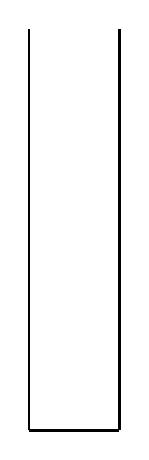
\begin{tikzpicture}[x=1cm,y=1cm]
								\def\W{1.15}
								\def\H{5.10}
								\def\cell{0.58}
								\draw[line width=0.9pt] (0,0) -- (0,\H);
								\draw[line width=0.9pt] (\W,0) -- (\W,\H);
								\draw[line width=0.9pt] (0,0) -- (\W,0);
								% stack rỗng (đúng như ảnh)
							\end{tikzpicture}
						\end{flushright}
					\end{columns}
				\end{frame}
				
				%========================
				% SLIDE 34
				%========================
				\begin{frame}[t]{Minh hoạ}
					\setlength{\leftmargini}{-1.2em}
					\small
					
					\begin{columns}[T,onlytextwidth]
						\column{0.72\textwidth}
						\begin{itemize}
							\item \textbf{Minh hoạ số 2: dãy ngoặc \texttt{()[(\}\})]}}
							\begin{itemize}
								\item Bước 1: Gặp ngoặc tiếp theo là ngoặc mở ``('' $\rightarrow$ đưa ngoặc mở này\\
								vào ngăn xếp
								\item Bước 2: Gặp ngoặc tiếp theo là ngoặc đóng ``)'' $\rightarrow$ lấy 1 ngoặc mở là\\
								``('' ra khỏi ngăn xếp
								\begin{itemize}
									\item So khớp ``('' ``)'' $\rightarrow$ kết quả đúng nên ta duyệt tiếp
								\end{itemize}
								\item Bước 3: Gặp ngoặc tiếp theo là ngoặc mở ``['' $\rightarrow$ đưa ngoặc mở này\\
								vào ngăn xếp
							\end{itemize}
						\end{itemize}
						
						\column{0.28\textwidth}
						\vspace{0.55cm}
						\begin{flushright}
							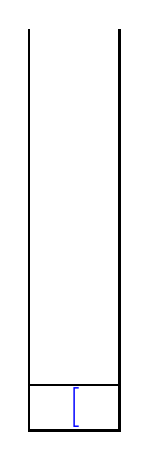
\begin{tikzpicture}[x=1cm,y=1cm]
								\def\W{1.15}
								\def\H{5.10}
								\def\cell{0.58}
								\draw[line width=0.9pt] (0,0) -- (0,\H);
								\draw[line width=0.9pt] (\W,0) -- (\W,\H);
								\draw[line width=0.9pt] (0,0) -- (\W,0);
								
								\draw[line width=0.9pt] (0,0) rectangle (\W,\cell);
								\node[font=\Large] at (\W/2,0.5*\cell) {\textcolor{blue}{[}};
							\end{tikzpicture}
						\end{flushright}
					\end{columns}
				\end{frame}
				
				%========================
				% SLIDE 35
				%========================
				\begin{frame}[t]{Minh hoạ}
					\setlength{\leftmargini}{-1.2em}
					\small
					
					\begin{columns}[T,onlytextwidth]
						\column{0.72\textwidth}
						\begin{itemize}
							\item \textbf{Minh hoạ số 2: dãy ngoặc \texttt{()[(\}\})]}}
							\begin{itemize}
								\item Bước 1: Gặp ngoặc tiếp theo là ngoặc mở ``('' $\rightarrow$ đưa ngoặc mở này\\
								vào ngăn xếp
								\item Bước 2: Gặp ngoặc tiếp theo là ngoặc đóng ``)'' $\rightarrow$ lấy 1 ngoặc mở là\\
								``('' ra khỏi ngăn xếp
								\begin{itemize}
									\item So khớp ``('' ``)'' $\rightarrow$ kết quả đúng nên ta duyệt tiếp
								\end{itemize}
								\item Bước 3: Gặp ngoặc tiếp theo là ngoặc mở ``['' $\rightarrow$ đưa ngoặc mở này\\
								vào ngăn xếp
								\item Bước 4: Gặp ngoặc tiếp theo là ngoặc mở ``('' $\rightarrow$ đưa ngoặc\\
								mở này vào ngăn xếp
							\end{itemize}
						\end{itemize}
						
						\column{0.28\textwidth}
						\vspace{0.55cm}
						\begin{flushright}
							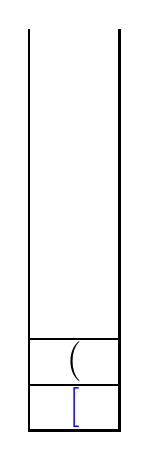
\begin{tikzpicture}[x=1cm,y=1cm]
								\def\W{1.15}
								\def\H{5.10}
								\def\cell{0.58}
								\draw[line width=0.9pt] (0,0) -- (0,\H);
								\draw[line width=0.9pt] (\W,0) -- (\W,\H);
								\draw[line width=0.9pt] (0,0) -- (\W,0);
								
								% bottom: [
								\draw[line width=0.9pt] (0,0) rectangle (\W,\cell);
								\node[font=\Large] at (\W/2,0.5*\cell) {\textcolor{blue}{[}};
								% top: (
								\draw[line width=0.9pt] (0,\cell) rectangle (\W,2*\cell);
								\node[font=\Large] at (\W/2,1.5*\cell) {(};
							\end{tikzpicture}
						\end{flushright}
					\end{columns}
				\end{frame}
				
				%========================
				% SLIDE 36
				%========================
				\begin{frame}[t]{Minh hoạ}
					\setlength{\leftmargini}{-1.2em}
					\small
					
					\begin{columns}[T,onlytextwidth]
						\column{0.72\textwidth}
						\begin{itemize}
							\item \textbf{Minh hoạ số 2: dãy ngoặc \texttt{()[(\}\})]}}
							\begin{itemize}
								\item Bước 1: Gặp ngoặc tiếp theo là ngoặc mở ``('' $\rightarrow$ đưa ngoặc mở này\\
								vào ngăn xếp
								\item Bước 2: Gặp ngoặc tiếp theo là ngoặc đóng ``)'' $\rightarrow$ lấy 1 ngoặc mở là\\
								``('' ra khỏi ngăn xếp
								\begin{itemize}
									\item So khớp ``('' ``)'' $\rightarrow$ kết quả đúng nên ta duyệt tiếp
								\end{itemize}
								\item Bước 3: Gặp ngoặc tiếp theo là ngoặc mở ``['' $\rightarrow$ đưa ngoặc mở này\\
								vào ngăn xếp
								\item Bước 4: Gặp ngoặc tiếp theo là ngoặc mở ``('' $\rightarrow$ đưa ngoặc\\
								mở này vào ngăn xếp
								\item Bước 5: Gặp ngoặc tiếp theo là ngoặc đóng ``\}'' $\rightarrow$ lấy 1 ngoặc\\
								mở là ngoặc ``('' ra
							\end{itemize}
						\end{itemize}
						
						\column{0.28\textwidth}
						\vspace{0.55cm}
						\begin{flushright}
							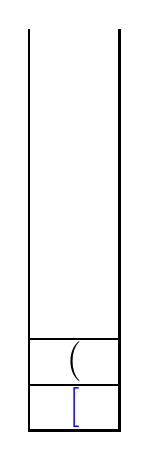
\begin{tikzpicture}[x=1cm,y=1cm]
								\def\W{1.15}
								\def\H{5.10}
								\def\cell{0.58}
								\draw[line width=0.9pt] (0,0) -- (0,\H);
								\draw[line width=0.9pt] (\W,0) -- (\W,\H);
								\draw[line width=0.9pt] (0,0) -- (\W,0);
								
								% (đúng như ảnh 36: vẫn còn 2 ô)
								\draw[line width=0.9pt] (0,0) rectangle (\W,\cell);
								\node[font=\Large] at (\W/2,0.5*\cell) {\textcolor{blue}{[}};
								\draw[line width=0.9pt] (0,\cell) rectangle (\W,2*\cell);
								\node[font=\Large] at (\W/2,1.5*\cell) {(};
							\end{tikzpicture}
						\end{flushright}
					\end{columns}
				\end{frame}
				
				%========================
				% SLIDE 37 (kết luận sai)
				%========================
				\begin{frame}[t]{Minh hoạ}
					\setlength{\leftmargini}{-1.2em}
					\small
					
					\begin{columns}[T,onlytextwidth]
						\column{0.72\textwidth}
						\begin{itemize}
							\item Bước 4: Gặp ngoặc tiếp theo là ngoặc mở ``('' $\rightarrow$ đưa ngoặc mở này\\
							vào ngăn xếp
							\item Bước 5: Gặp ngoặc tiếp theo là ngoặc đóng ``\}'' $\rightarrow$ lấy 1 ngoặc mở là\\
							ngoặc ``('' ra
							\begin{itemize}
								\item So khớp ``('' ``\}'' $\rightarrow$ kết quả so khớp là sai nên ta kết luận dãy\\
								ngoặc đã cho không cân xứng
							\end{itemize}
						\end{itemize}
						
						\column{0.28\textwidth}
						\vspace{0.55cm}
						\begin{flushright}
							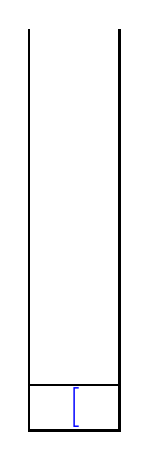
\begin{tikzpicture}[x=1cm,y=1cm]
								\def\W{1.15}
								\def\H{5.10}
								\def\cell{0.58}
								\draw[line width=0.9pt] (0,0) -- (0,\H);
								\draw[line width=0.9pt] (\W,0) -- (\W,\H);
								\draw[line width=0.9pt] (0,0) -- (\W,0);
								
								% Sau khi pop '(' còn lại '['
								\draw[line width=0.9pt] (0,0) rectangle (\W,\cell);
								\node[font=\Large] at (\W/2,0.5*\cell) {\textcolor{blue}{[}};
							\end{tikzpicture}
						\end{flushright}
					\end{columns}
				\end{frame}
				
				
	
	
	
	
	\begin{frame}[t,fragile]{Cài đặt thuật toán}
		\setlength{\leftmargini}{-1.2em}
		
		\vspace{-0.35cm}
		\hspace{0.85cm}
		\begin{tcolorbox}[
			width=0.52\textwidth,
			colback=white,
			colframe=blue!55!black,
			boxrule=0.6pt,
			arc=0pt,
			left=-34pt,right=10pt,top=10pt,bottom=10pt
			]
			\begin{minted}[fontsize=\scriptsize, breaklines, linenos=false]{c}
				#include <stdio.h>
				#include <string.h>
				#include <stdlib.h>
				
				typedef struct Node{
					char c;
					struct Node* next;
				}Node;
				
				Node* top;
				char s[1000001];
				
				Node* makeNode(char c){
					Node* p=(Node*)malloc(sizeof(Node));
					p->c = c; p->next = NULL; return p;
				}
			\end{minted}
		\end{tcolorbox}
	\end{frame}
	
	\begin{frame}[t,fragile]{Cài đặt thuật toán}
		\setlength{\leftmargini}{-1.2em}
		
		\vspace*{-0.6cm}
		\begin{columns}[T,onlytextwidth]
			%================ LEFT COLUMN ================%
			\begin{column}{0.54\textwidth}
				\begin{tcolorbox}[
					width=\textwidth,
					colback=white,
					colframe=blue!55!black,
					boxrule=0.6pt,
					arc=0pt,
					left=-20pt,right=10pt,top=10pt,bottom=10pt
					]
					\begin{minted}[fontsize=\scriptsize, breaklines, linenos=false]{c}
						#include <stdio.h>
						#include <string.h>
						#include <stdlib.h>
						
						typedef struct Node{
							char c;
							struct Node* next;
						}Node;
						
						Node* top;
						char s[1000001];
						
						Node* makeNode(char c){
							Node* p=(Node*)malloc(sizeof(Node));
							p->c = c; p->next = NULL; return p;
						}
					\end{minted}
				\end{tcolorbox}
			\end{column}
			
			%================ RIGHT COLUMN ================%
			\begin{column}{0.42\textwidth}
				\begin{tcolorbox}[
					width=\textwidth,
					colback=white,
					colframe=blue!55!black,
					boxrule=0.6pt,
					arc=0pt,
					left=-20pt,right=10pt,top=10pt,bottom=10pt
					]
					\begin{minted}[fontsize=\scriptsize, breaklines, linenos=false]{c}
						void push(char c){
							Node* p = makeNode(c);
							p->next = top; top = p;
						}
						
						char pop(){
							if(top == NULL) return ' ';
							Node* tmp = top; top = top->next;
							char res = tmp->c;
							free(tmp);
							return res;
						}
					\end{minted}
				\end{tcolorbox}
			\end{column}
		\end{columns}
	\end{frame}
	
	%================== SLIDE 40 ==================%
	\begin{frame}[t,fragile]{Cài đặt thuật toán}
		\setlength{\leftmargini}{-1.2em}
		
		\vspace{-0.35cm}
		\begin{tcolorbox}[
			width=0.52\textwidth,
			colback=white,
			colframe=blue!55!black,
			boxrule=0.6pt,
			arc=0pt,
			left=-20pt,right=10pt,top=10pt,bottom=10pt
			]
			\begin{minted}[fontsize=\scriptsize, breaklines, linenos=false]{c}
				int match(char a, int b){
					if(a == '(' && b == ')') return 1;
					if(a == '{' && b == '}') return 1;
					if(a == '[' && b == ']') return 1;
					return 0;
				}
			\end{minted}
		\end{tcolorbox}
	\end{frame}
	
	%================== SLIDE 41 ==================%
	\begin{frame}[t,fragile]{Cài đặt thuật toán}
		\setlength{\leftmargini}{-1.2em}
		
		\vspace{-0.6cm}
		\begin{columns}[T,onlytextwidth]
			%================ LEFT COLUMN ================%
			\begin{column}{0.45\textwidth}
				\begin{tcolorbox}[
					width=\textwidth,
					colback=white,
					colframe=blue!55!black,
					boxrule=0.6pt,
					arc=0pt,
					left=-20pt,right=10pt,top=10pt,bottom=10pt
					]
					\begin{minted}[fontsize=\scriptsize, breaklines, linenos=false]{c}
						int match(char a, int b){
							if(a == '(' && b == ')') return 1;
							if(a == '{' && b == '}') return 1;
							if(a == '[' && b == ']') return 1;
							return 0;
						}
					\end{minted}
				\end{tcolorbox}
			\end{column}
			
			%================ RIGHT COLUMN ================%
			\begin{column}{0.45\textwidth}
				\begin{tcolorbox}[
					width=\textwidth,
					colback=white,
					colframe=blue!55!black,
					boxrule=0.6pt,
					arc=0pt,
					left=-20pt,right=10pt,top=10pt,bottom=10pt
					]
					\begin{minted}[fontsize=\scriptsize, breaklines, linenos=false]{c}
						int check(char* s){
							for(int i = 0; i < strlen(s); i++){
								if(s[i] == '(' || s[i] == '{' || s[i] == '[')
									push(s[i]);
									else{
										if(top==NULL) return 0;
										char o = pop();
										if(!match(o,s[i])) return 0;
									}
								}
								return top == NULL;
							}
						\end{minted}
					\end{tcolorbox}
				\end{column}
			\end{columns}
		\end{frame}
		
		%================== SLIDE 42 ==================%
		\begin{frame}[t,fragile]{Cài đặt thuật toán}
			\setlength{\leftmargini}{-1.2em}
			
			\vspace{-0.65cm}
			\begin{columns}[T,onlytextwidth]
				%================ LEFT COLUMN (2 BOX) ================%
				\begin{column}{0.45\textwidth}
					% --- BOX 1: match ---
					\begin{tcolorbox}[
						width=\textwidth,
						height=0.38\textheight,
						colback=white,
						colframe=blue!55!black,
						boxrule=0.6pt,
						arc=0pt,
						left=-20pt,right=10pt,top=1pt,bottom=10pt
						]
						\begin{minted}[fontsize=\scriptsize, breaklines, linenos=false]{c}
							int match(char a, int b){
								if(a == '(' && b == ')') return 1;
								if(a == '{' && b == '}') return 1;
								if(a == '[' && b == ']') return 1;
								return 0;
							}
						\end{minted}
					\end{tcolorbox}
					
					\vspace{-0.05cm}
					
					% --- BOX 2: main ---
					\begin{tcolorbox}[
						width=\textwidth,
						height=0.33\textheight,
						colback=white,
						colframe=blue!55!black,
						boxrule=0.6pt,
						arc=0pt,
						left=-20pt,right=10pt,top=1pt,bottom=10pt
						]
						\begin{minted}[fontsize=\scriptsize, breaklines, linenos=false]{c}
							int main(){
								scanf("%s",s);
	
								int res = check(s);
								printf("%d",res);
								return 0;
							}
						\end{minted}
					\end{tcolorbox}
				\end{column}
				
				%================ RIGHT COLUMN (1 BOX) ================%
				\begin{column}{0.45\textwidth}
					\begin{tcolorbox}[
						width=\textwidth,
						colback=white,
						colframe=blue!55!black,
						boxrule=0.6pt,
						arc=0pt,
						left=-30pt,right=10pt,top=10pt,bottom=10pt
						]
						\begin{minted}[fontsize=\scriptsize, breaklines, linenos=false]{c}
							int check(char* s){
								for(int i = 0; i < strlen(s); i++){
									if(s[i] == '(' || s[i] == '{' || s[i] == '[')
										push(s[i]);
										else{
											if(top==NULL) return 0;
											char o = pop();
											if(!match(o,s[i])) return 0;
										}
									}
									return top == NULL;
								}
							\end{minted}
						\end{tcolorbox}
					\end{column}
				\end{columns}
			\end{frame}
			
		\section{Hàng đợi}
		
		\begin{frame}[t]{Giới thiệu hàng đợi}
			\definecolor{queueFill}{RGB}{129, 227, 189}
			\definecolor{queueDraw}{RGB}{15, 89, 75}
			\setlength{\leftmargini}{-1.2em}
			
			\vspace{-0.4cm}
			
			\begin{columns}[T]
				% --- CỘT TRÁI: LÝ THUYẾT ---
				\begin{column}{0.55\textwidth}
					\begin{itemize}
						
						\item Hàng đợi là một cấu trúc dữ liệu tuyến tính có hai đầu, \textcolor{red}{head} và \textcolor{red}{tail}.
						
						\item Thao tác thêm mới phần tử được thực hiện ở \textcolor{red}{tail}. Thao tác loại bỏ phần tử được thực hiện ở \textcolor{red}{head}.
						
						\item Nguyên tắc hoạt động: FIFO -- First In First Out.
						
						\item Thao tác cơ bản trên hàng đợi $Q$:
						\begin{itemize}
							\setlength{\itemsep}{0.5em}
							\item $enqueue(x, Q)$: chèn 1 phần tử $x$ vào hàng đợi
							\item $dequeue(Q)$: lấy ra 1 phần tử khỏi hàng đợi
							\item $isEmpty(Q)$: trả về true nếu hàng đợi rỗng
						\end{itemize}
					\end{itemize}
				\end{column}
				
				% --- CỘT PHẢI: HÌNH VẼ MINH HỌA ---
				\begin{column}{0.45\textwidth}
					\vspace{0.5cm}
					\centering
					
					\begin{adjustbox}{width=\linewidth}
						\begin{tikzpicture}[
							node distance=0pt,
							% Style cho các ô vuông (giữ nguyên)
							qnode/.style={
								draw=queueDraw, fill=queueFill, thick,
								minimum size=1cm, rounded corners=4pt,
								font=\sffamily\bfseries\large, text=queueDraw,
								inner sep=0pt, outer sep=0pt
							},
							% Style mũi tên: Thêm rounded corners cho mượt, chỉnh đầu mũi tên to hơn
							myarrow/.style={
								->, >=Stealth, line width=2.5pt, draw=queueDraw, rounded corners=8pt
							},
							% Style nhãn
							mylabel/.style={
								font=\sffamily\bfseries\scriptsize, text=queueDraw, align=center
							}
							]
							
							% --- HÀNG ĐỢI CHÍNH ---
							\node[qnode] (n3) {3};
							\node[qnode, right=0cm of n3] (n4) {4};
							\node[qnode, right=0cm of n4] (n5) {5};
							\node[qnode, right=0cm of n5] (n6) {6};
							\node[qnode, right=0cm of n6] (n7) {7};
							\node[qnode, right=0cm of n7] (n8) {8};
							
							% Nhãn Front/Head và Back/Tail
							\node[mylabel, above=0.15cm of n3] {Front / Head};
							\node[mylabel, above=0.15cm of n8] {Back / Tail / Rear};
							
							% --- PHẦN DEQUEUE (Bên trái) ---
							% Đẩy node 2 xa hơn về bên trái và xuống dưới
							\node[qnode, below left=1.2cm and 1.2cm of n3] (n2) {2};
							
							% Vẽ mũi tên: Đi từ cạnh trái n3 -> Sang trái -> Cắm xuống đầu n2
							% Sử dụng -| để vẽ đường vuông góc tự động
							\draw[myarrow] (n3.west) -| (n2.north);
							
							% Nhãn Dequeue: Đặt bên trái của đoạn thẳng đứng (tránh đè lên dây)
							\node[mylabel, anchor=east] at ([xshift=-0.1cm, yshift=0.8cm]n2.north) {Dequeue};
							
							% --- PHẦN ENQUEUE (Bên phải) ---
							% Đẩy node 9 xa hơn về bên phải và lên trên
							\node[qnode, above right=1.2cm and 1.2cm of n8] (n9) {9};
							
							% Vẽ mũi tên: Đi từ đáy n9 -> Xuống dưới -> Rẽ sang n8
							% Sử dụng |- để vẽ đường vuông góc tự động
							\draw[myarrow] (n9.south) |- (n8.east);
							
							% Nhãn Enqueue: Đặt bên phải của đoạn thẳng đứng (tránh đè lên dây)
							\node[mylabel, anchor=west] at ([xshift=0.1cm, yshift=-0.8cm]n9.south) {Enqueue};
							
						\end{tikzpicture}
					\end{adjustbox}
					
					\vspace{0.5cm}
					\textit{Ý tưởng hoạt động của hàng đợi}
					
				\end{column}
			\end{columns}
			
			\vfill
			\raggedleft
			\tiny \textit{Nguồn: \href{https://www.geeksforgeeks.org/queue-data-structure/}{https://www.geeksforgeeks.org/queue-data-structure/}}
			
		\end{frame}
		
		% ==================================================================
		\begin{frame}{Minh họa hoạt động của hàng đợi}
			\centering
			\small 
			\renewcommand{\arraystretch}{1.15}
			\begin{adjustbox}{width=0.85\textwidth} 
				\begin{tabular}{|p{4.5cm}|p{3.0cm}|c|}
					\hline
					% Tiêu đề
					\centering\textbf{Thao tác} & 
					\textbf{Trạng thái \newline hàng đợi} & 
					\parbox{3cm}{\centering\textbf{Phần tử trả \newline về nếu có}} \\
					\hline
					
					% Nội dung
					Create an empty queue & Empty      & - \\ \hline
					Enqueue 1             & 1          & - \\ \hline
					Enqueue 2             & 1, 2       & - \\ \hline
					Enqueue 3             & 1, 2, 3    & - \\ \hline
					Dequeue               & 2, 3       & 1 \\ \hline
					Enqueue 4             & 2, 3, 4    & - \\ \hline
					Enqueue 5             & 2, 3, 4, 5 & - \\ \hline
					Dequeue               & 3, 4, 5    & 2 \\ \hline
					Dequeue               & 4, 5       & 3 \\ \hline
					Check if empty        & 4, 5       & 0 \\ \hline
				\end{tabular}
			\end{adjustbox}
		\end{frame}
		
		%================== SLIDE 46 ==================%
		\begin{frame}[t,fragile]{Cài đặt hàng đợi sử dụng danh sách liên kết đơn}
			\setlength{\leftmargini}{-1.2em}
			\small
			
			\begin{itemize}
				\item Cấu trúc và hàm khởi tạo thành phần
			\end{itemize}
			
			\vspace{0.15cm}
			
			\begin{tikzpicture}[remember picture]
				% --- Code box (left) ---
				\node (codebox) [anchor=north west, inner sep=0pt] at (0,0) {%
					\begin{tcolorbox}[
						width=0.58\textwidth,
						height=0.54\textheight,
						colback=white,
						colframe=blue!55!black,
						boxrule=0.6pt,
						arc=0pt,
						left=8pt,right=8pt,top=8pt,bottom=8pt
						]
						\begin{minted}[fontsize=\scriptsize, breaklines, linenos=false]{c}
							typedef struct Node{
								char value;
								struct Node* next;
							}Node;
							
							Node* makeNode(char v){
								Node* p = (Node*)malloc(sizeof(Node));
								p->value = v;
								p->next  = NULL;
								return p;
							}
						\end{minted}
					\end{tcolorbox}
				};
				
				% --- Callout boxes (right) ---
				\node (note1) [draw, rectangle, thick, align=center, font=\scriptsize,
				minimum width=0.34\textwidth, minimum height=1.25cm,
				anchor=west]
				at ($(codebox.north east)+(1.05cm,-1.25cm)$)
				{Khai báo struct cho một phần tử\\của hàng đợi};
				
				\node (note2) [draw, rectangle, thick, align=center, font=\scriptsize,
				minimum width=0.34\textwidth, minimum height=1.25cm,
				anchor=west]
				at ($(codebox.north east)+(1.05cm,-4.00cm)$)
				{Tạo một phần tử (node) của hàng\\đợi};
				
				% ====== ARROWS (mũi tên đơn, thẳng ngang) ======
				\tikzset{myarr/.style={->,>=Stealth,line width=0.85pt,shorten <=2pt,shorten >=2pt}}
				
				\coordinate (T1) at (codebox.east |- note1.west);
				\coordinate (T2) at (codebox.east |- note2.west);
				
				% vẽ từ note sang code (đầu mũi tên ở phía codebox)
				\draw[myarr] (note1.west) -- (T1);
				\draw[myarr] (note2.west) -- (T2);
				
			\end{tikzpicture}
		\end{frame}
		
		% \begin{frame}[t,fragile]{Cài đặt hàng đợi sử dụng danh sách liên kết đơn}
		% 	\setlength{\leftmargini}{-1.2em}
		% 	\large
		% 	\begin{itemize}
		% 		\item Thao tác Enqueue
		% 	\end{itemize}
			
		% 	\vspace{0.15cm}
			
		% 	\begin{tikzpicture}[remember picture]
		% 		% --- Code box (left) ---
		% 		\node (codebox) [anchor=north west, inner sep=0pt] at (0,0) {%
		% 			\begin{tcolorbox}[
		% 				width=0.62\textwidth,
		% 				height=0.60\textheight,
		% 				colback=white,
		% 				colframe=blue!55!black,
		% 				boxrule=0.6pt,
		% 				arc=0pt,
		% 				left=6pt,right=6pt,top=6pt,bottom=6pt
		% 				]
		% 				\begin{minted}[fontsize=\scriptsize, breaklines, linenos=false, escapeinside=||]{c}
		% 					Node* enqueue(Node* head, char v){
		% 						Node* new_node = makeNode(v);|\tikz[remember picture,overlay]\node (mkMake) {};|
								
		% 						if(head == NULL) return new_node;|\tikz[remember picture,overlay]\node (mkRet) {};|
								
		% 						else{
		% 							|\tikz[remember picture,overlay]\node (blkTL) {};|new_node->next = head;|\tikz[remember picture,overlay]\node (mkElse) {};|
		% 							head = new_node;
		% 							return head;|\tikz[remember picture,overlay]\node (blkBR) {};|
		% 						}
		% 					}
		% 				\end{minted}
		% 			\end{tcolorbox}
		% 		};
				
		% 		% --- Callout boxes (right) ---
		% 		\node (note1) [draw, rectangle, thick, align=center, font=\scriptsize,
		% 		minimum width=0.30\textwidth, minimum height=0.90cm,
		% 		anchor=west]
		% 		at ($(codebox.north east)+(0.95cm,-1.15cm)$)
		% 		{Tạo một node mới};
				
		% 		\node (note2) [draw, rectangle, thick, align=center, font=\scriptsize,
		% 		minimum width=0.30\textwidth, minimum height=1.20cm,
		% 		anchor=west]
		% 		at ($(codebox.north east)+(0.95cm,-2.75cm)$)
		% 		{Nếu hàng đợi rỗng, trả về\\phần tử mới tạo};
				
		% 		\node (note3) [draw, rectangle, thick, align=center, font=\scriptsize,
		% 		minimum width=0.30\textwidth, minimum height=1.80cm,
		% 		anchor=west]
		% 		at ($(codebox.north east)+(0.95cm,-4.65cm)$)
		% 		{Nếu hàng đợi không rỗng, biến\\node mới tạo thành phần tử\\đầu danh sách};
				
		% 		% ====== GREEN HIGHLIGHT BOX: dùng FIT để ôm đúng khối else ======
		% 		\coordinate (fitTL) at ([xshift=-6pt,yshift=6pt]blkTL);
		% 		\coordinate (fitBR) at ([xshift=38pt,yshift=-6pt]blkBR);
		% 		\node[draw=green!60!black, line width=1pt,
		% 		fit=(fitTL)(fitBR)] (gbox) {};
				
		% 		% ====== ARROWS: NOTE -> CODE (cắm đúng) ======
		% 		\tikzset{myarr/.style={-Stealth, line width=0.85pt}}
				
		% 		% đích (bạn có thể chỉnh xshift/yshift để trỏ chuẩn hơn)
		% 		\coordinate (tMake) at ([xshift=-6pt,yshift=0pt]mkMake);
		% 		\coordinate (tRet)  at ([xshift=-6pt,yshift=0pt]mkRet);
		% 		\coordinate (tElse) at ([xshift=-6pt,yshift=0pt]mkElse);
				
		% 		% vẽ: xuất phát luôn từ đúng note (không dùng |- nữa)
		% 		\draw[myarr] (note1.west) to[out=180,in=0,looseness=1.15] (tMake);
		% 		\draw[myarr] (note2.west) to[out=180,in=0,looseness=1.15] (tRet);
		% 		\draw[myarr] (note3.west) to[out=180,in=0,looseness=1.15] (tElse);
		% 	\end{tikzpicture}
		% \end{frame}
		
	% \begin{frame}[t,fragile]{Cài đặt hàng đợi sử dụng danh sách liên kết đơn}
	% 	\setlength{\leftmargini}{-1.2em}
		
	% 	\vspace{-0.25cm}
	% 	\begin{columns}[T,onlytextwidth]
	% 		% ====== COL 1: bullet (trái) ======
	% 		\begin{column}{0.2\textwidth}
	% 			\large
	% 			\begin{itemize}
	% 				\item Thao tác Dequeue
	% 			\end{itemize}
	% 		\end{column}
			
	% 		% ====== COL 2: code (giữa) ======
	% 		\begin{column}{0.42\textwidth}
	% 			\vspace{-0.05cm}
	% 			\begin{tikzpicture}[remember picture]
	% 				\node (codebox) [anchor=north west, inner sep=0pt] at (0,0) {%
	% 					\begin{tcolorbox}[
	% 						width=\linewidth,
	% 						% KHÔNG set height cứng để tránh tràn
	% 						colback=white,
	% 						colframe=blue!55!black,
	% 						boxrule=0.6pt,
	% 						arc=0pt,
	% 						left=-60pt,right=6pt,top=6pt,bottom=6pt
	% 						]
	% 						\begin{minted}[fontsize=\scriptsize, breaklines, linenos=false, escapeinside=||]{c}
	% 							char dequeue(Node** head){
	% 								if(*head == NULL) return NULL;|\tikz[remember picture,overlay]\node[inner sep=0pt,outer sep=0pt] (mkEmpty) {};|
	% 								Node* p, *q;
	% 								p = *head;
	% 								char ans;
	% 								|\tikz[remember picture,overlay]\node[inner sep=0pt,outer sep=0pt] (blk1TL) {};|if(p->next == NULL){
	% 									ans = p->value;
	% 									free(p);
	% 									*head = NULL;
	% 									return ans;
	% 								}|\tikz[remember picture,overlay]\node[inner sep=0pt,outer sep=0pt] (blk1BR) {};|
	% 								|\tikz[remember picture,overlay]\node[inner sep=0pt,outer sep=0pt] (blk2TL) {};|while(p->next->next != NULL){
	% 									p = p->next;
	% 								}
	% 								q = p->next;
	% 								p->next = NULL;
	% 								ans = q->value;
	% 								free(q);
	% 								return ans;|\tikz[remember picture,overlay]\node[inner sep=0pt,outer sep=0pt] (blk2BR) {};|
	% 							}
	% 						\end{minted}
	% 					\end{tcolorbox}
	% 				};
					
	% 			\coordinate (g1TL) at ([xshift=-12pt,yshift=8pt]blk1TL);
	% 			\coordinate (g1BR) at ([xshift=90pt,yshift=-1pt]blk1BR);
	% 			\draw[green!60!black, line width=1.0pt] (g1TL) rectangle (g1BR);
				
	% 			% lấy điểm giữa + điểm cạnh phải để bắn mũi tên (KHÔNG dùng |-)
	% 			\coordinate (g1Mid) at ($(g1TL)!0.5!(g1BR)$);
	% 			\path let \p1=(g1BR), \p2=(g1Mid) in coordinate (g1Right) at (\x1,\y2);
				
	% 			% Box 2 (khối while... đến return)
	% 			\coordinate (g2TL) at ([xshift=-12pt,yshift=7pt]blk2TL);
	% 			\coordinate (g2BR) at ([xshift=90pt,yshift=-14pt]blk2BR);
	% 			\draw[green!60!black, line width=1.0pt] (g2TL) rectangle (g2BR);
				
	% 			\coordinate (g2Mid) at ($(g2TL)!0.5!(g2BR)$);
	% 			\path let \p1=(g2BR), \p2=(g2Mid) in coordinate (g2Right) at (\x1,\y2);
	% 			\end{tikzpicture}
	% 		\end{column}
			
	% 		% ====== COL 3: notes + arrows (phải) ======
	% 		% ====== COL 3: notes + arrows (phải) ======
	% 		\begin{column}{0.40\textwidth}
	% 			% để trống nội dung layout, vì note+arrow sẽ vẽ overlay theo tọa độ global
	% 			\vspace{0pt}
				
	% 			\begin{tikzpicture}[remember picture,overlay]
	% 				% ---- đặt note theo đúng cao độ của code (global) ----
	% 				% x = cạnh phải codebox + 1.05cm ; y = y của mkEmpty / g1Mid / g2Mid
	% 				\path let \p1=(codebox.east), \p2=(mkEmpty) in
	% 				coordinate (posN1) at (\x1+1.05cm,\y2);
	% 				\path let \p1=(codebox.east), \p2=(g1Mid) in
	% 				coordinate (posN2) at (\x1+1.05cm,\y2);
	% 				\path let \p1=(codebox.east), \p2=(g2Mid) in
	% 				coordinate (posN3) at (\x1+1.05cm,\y2);
					
	% 				\node (note1) [draw, rectangle, thick, align=center, font=\scriptsize,
	% 				text width=0.60\textwidth, minimum height=1.05cm,
	% 				anchor=west] at (posN1)
	% 				{Nếu hàng đợi rỗng, trả về rỗng};
					
	% 				\node (note2) [draw, rectangle, thick, align=center, font=\scriptsize,
	% 				text width=0.70\textwidth, minimum height=1.20cm,
	% 				anchor=west] at (posN2)
	% 				{Nếu hàng đợi chỉ có một phần tử};
					
	% 				\node (note3) [draw, rectangle, thick, align=center, font=\scriptsize,
	% 				text width=0.70\textwidth, minimum height=2.10cm,
	% 				anchor=west] at (posN3)
	% 				{Nếu hàng đợi có nhiều hơn một phần tử, lấy phần tử cuối cùng của danh sách};
					
	% 				% ---- ARROWS (không bị Dimension too large nữa) ----
	% 				\tikzset{myarr/.style={-Stealth, line width=0.85pt}}
					
	% 				\coordinate (tEmpty) at ([xshift=-2pt,yshift=3pt]mkEmpty);
	% 				\coordinate (tOne)   at ([xshift=0pt,yshift=0pt]g1Right);
	% 				\coordinate (tMany)  at ([xshift=0pt,yshift=0pt]g2Right);
					
	% 				% dùng đường cong theo format bạn muốn (không dùng |- khi vẽ)
	% 				\draw[myarr] (note1.west) to[out=180,in=0,looseness=1.10] (tEmpty);
	% 				\draw[myarr] (note2.west) to[out=180,in=0,looseness=1.10] (tOne);
	% 				\draw[myarr] (note3.west) to[out=180,in=0,looseness=1.10] (tMany);
	% 			\end{tikzpicture}
	% 		\end{column}
			
			
	% 	\end{columns}
	% \end{frame}
	
		
		
		
		%========================
		% Slide 49
		%========================
		\begin{frame}[t]{Một số ứng dụng của hàng đợi}
			\setlength{\leftmargini}{-1.2em}
			\small
			
			\begin{itemize}
				\item \textbf{Tìm kiếm theo chiều rộng (BFS):} BFS là một thuật toán để duyệt hoặc tìm kiếm trong cấu trúc dữ liệu cây và đồ thị. Nó sử dụng một hàng đợi để khám phá các nút theo từng cấp độ, làm cho nó trở thành công cụ quan trọng để giải quyết các vấn đề liên quan đến đồ thị.
				
				\vspace{0.35cm}
				
				\item \textbf{Lập lịch công việc (Task scheduling):} Hàng đợi được sử dụng trong các hệ điều hành để lên lịch cho các tác vụ hoặc tiến trình để thực thi. Các tác vụ được đặt vào hàng đợi và hệ điều hành thực hiện chúng theo thứ tự chúng được thêm vào, đảm bảo sự công bằng trong phân phối tài nguyên.
			\end{itemize}
		\end{frame}
		
		%========================
		% Slide 50
		%========================
		\begin{frame}[t]{Một số ứng dụng của hàng đợi}
			\setlength{\leftmargini}{-1.2em}
			\small
			
			\begin{itemize}
				\item \textbf{Xử lý yêu cầu trên máy chủ web (Web server request handling):} Các máy chủ web sử dụng hàng đợi để quản lý các yêu cầu HTTP đến. Mỗi yêu cầu đến được đặt vào hàng đợi và xử lý bởi các luồng hoặc tiến trình làm việc, cho phép máy chủ xử lý nhiều yêu cầu cùng một lúc
				
				\vspace{0.35cm}
				
				\item \textbf{Đệm trong các hoạt động I/O (Buffering in I/O operations):} Hàng đợi được sử dụng để đệm dữ liệu trong các hoạt động I/O. Ví dụ, khi dữ liệu được đọc từ tệp hoặc ổ đĩa mạng, thường được đặt vào hàng đợi trước khi xử lý để làm dịu sự biến đổi trong tốc độ nhận dữ liệu.
			\end{itemize}
		\end{frame}
		
		%========================
		% Slide 51
		%========================
		\begin{frame}[t]{Một số ứng dụng của hàng đợi}
			\setlength{\leftmargini}{-1.2em}
			\small
			
			\begin{itemize}
				\item \textbf{Quản lý tác vụ trong ứng dụng đa luồng (Task management in multithreading):} Trong các ứng dụng đa luồng, hàng đợi có thể được sử dụng để quản lý các tác vụ cần được thực thi đồng thời. Các luồng thực hiện bóc tác vụ từ hàng đợi và thực hiện công việc tương ứng.
				
				\vspace{0.55cm}
				
				\item \textbf{Xử lý đơn đặt hàng trong kho(Order fulfillment in warehouses):}\\
				Trong quản lý logistics và kho lưu trữ, hàng đợi có thể được sử dụng để quản lý quy trình thực hiện đơn đặt hàng. Đơn đặt hàng được đặt vào hàng đợi để lựa chọn, đóng gói và giao hàng để đảm bảo xử lý hiệu quả.
			\end{itemize}
		\end{frame}
		
		\section{Bài tập: Tìm đường đi nhanh nhất thoát khỏi mê cung}
		
		% ==================================================================
		% SLIDE: ĐỀ BÀI (MÊ CUNG)
		% ==================================================================
		\begin{frame}[t]{Đề bài}
			\setlength{\leftmargini}{-1.2em}
			\small
			% Phần văn bản đề bài
			\begin{itemize}
				\item \textbf{Đề bài:} Một mê cung hình chữ nhật được biểu diễn bởi 0-1 ma trận $N \times M$ trong đó $A[i,j] = 1$ thể hiện ô $(i,j)$ là tường gạch và $A[i,j] = 0$ thể hiện ô $(i,j)$ là ô trống, có thể di chuyển vào. Từ 1 ô trống, ta có thể di chuyển sang 1 trong 4 ô lân cận (lên trên, xuống dưới, sang trái, sang phải) nếu ô đó là ô trống.
			\end{itemize}
			
			
			\begin{columns}[T]
				% --- CỘT TRÁI: YÊU CẦU ---
				\begin{column}{0.4\textwidth}
					\vspace{0.5cm}
					\begin{itemize}
						\item Xuất phát từ 1 ô trống trong mê cung, hãy tìm đường ngắn nhất thoát ra khỏi mê cung.
					\end{itemize}
				\end{column}
				
				% --- CỘT PHẢI: HÌNH VẼ MÊ CUNG ---
				\begin{column}{0.56\textwidth}
					\centering
					\begin{adjustbox}{width=0.75\linewidth}
						\begin{tikzpicture}[x=0.5cm, y=0.5cm]
							% Định nghĩa số hàng và số cột
							\def\rows{8}
							\def\cols{12}
							
							% Vẽ lưới ô vuông
							\draw[step=1, gray, thin] (1, -\rows) grid (\cols+1, 0);
							
							% Đánh số cột (1 -> 12)
							\foreach \c in {1,...,12} {
								\node[anchor=south, font=\scriptsize] at (\c + 0.5, 0) {\c};
							}
							
							% Đánh số hàng (1 -> 8)
							\foreach \r in {1,...,8} {
								\node[anchor=east, font=\scriptsize] at (1, -\r + 0.5) {\r};
							}
							
							% --- TÔ MÀU CÁC Ô TƯỜNG (MÀU ĐEN) ---
							% Tọa độ (cột, hàng) - Lưu ý: trong TikZ y đi lên nên ta dùng số âm cho hàng
							\foreach \c/\r in {
								% Hàng 1
								1/1, 2/1, 7/1, 12/1,
								% Hàng 2
								1/2, 5/2, 6/2, 8/2, 11/2, 12/2,
								% Hàng 3
								3/3,
								% Hàng 4
								1/4, 7/4, 10/4, 12/4,
								% Hàng 5
								1/5, 4/5, 10/5,
								% Hàng 6
								1/6, 3/6, 5/6, 9/6, 11/6,
								% Hàng 7
								5/7, 7/7,
								% Hàng 8
								1/8, 4/8, 3/8, 6/8, 7/8, 8/8, 10/8, 12/8
							} {
								\fill[black] (\c, -\r) rectangle ++(1, 1);
							}
							
							% --- VẼ ĐƯỜNG ĐI (MÀU ĐỎ) ---
							% Điểm xuất phát X tại (5, 5)
							\node[font=\bfseries\small] at (6.5, -4.5) {X};
							
							% Vẽ mũi tên gấp khúc
							\draw[->, >=Stealth, red, line width=1.5pt] 
							(6.7, -4.5) -- (7.5, -4.5)  % Sang phải ô 6
							-- (7.5, -5.5)              % Xuống ô 6 (hàng 6)
							-- (8.5, -5.5)              % Sang phải ô 7
							-- (8.5, -6.5)              % Xuống ô 7 (hàng 7)
							-- (9.5, -6.5)              % Sang phải ô 8
							-- (9.5, -7.5)              % Xuống ô 8 (hàng 8)
							-- (9.5, -8.8);             % Thoát ra ngoài
							
							% Nhãn "7 bước"
							\node[red, font=\small] at (9.5, -9.2) {7 bước};
							
						\end{tikzpicture}
					\end{adjustbox}
				\end{column}
			\end{columns}
		\end{frame}
		
		%========================
		% Slide 54
		%========================
		\begin{frame}[t]{Đề bài}
			\setlength{\leftmargini}{-1.2em}
			\large
			
			\begin{itemize}
				\item \textcolor{blue}{\textbf{Dữ liệu đầu vào:}}
				\begin{itemize}
					\item Dòng 1: ghi 4 số nguyên dương n, m, r, c trong đó n và m tương ứng là số hàng và cột của ma\\
					trận A ($1 \le n,m \le 999$) và r, c tương ứng là chỉ số hàng, cột của ô xuất phát.
					
					\vspace{0.2cm}
					
					\item Dòng i+1 (i=1,...,n): ghi dòng thứ i của ma trận A
				\end{itemize}
				
				\vspace{0.35cm}
				
				\item \textcolor{blue}{\textbf{Kết quả đầu ra:}}
				\begin{itemize}
					\item Ghi ra số bước cần di chuyển ngắn nhất để thoát ra khỏi mê cung, hoặc ghi giá trị $-1$ nếu không\\
					tìm thấy đường đi nào thoát ra mê cung.
				\end{itemize}
			\end{itemize}
		\end{frame}
		
		%========================
		% Slide 55 (FIXED)
		%========================
		\begin{frame}[t]{Đề bài}
			\setlength{\leftmargini}{-1.2em}
			\large
			
			\begin{columns}[T,onlytextwidth]
				% -------- LEFT TEXT --------
				\column{0.62\textwidth}
				\begin{itemize}
					\item \textcolor{blue}{\textbf{Dữ liệu đầu vào:}}
					\begin{itemize}
						\item Dòng 1: ghi 4 số nguyên dương n, m, r, c trong đó\\
						n và m tương ứng là số hàng và cột của ma trận A\\
						($1 \le n,m \le 999$) và r, c tương ứng là chỉ số hàng,\\
						cột của ô xuất phát.
						\vspace{0.2cm}
						\item Dòng i+1 (i=1,...,n): ghi dòng thứ i của ma trận A
					\end{itemize}
					
					\vspace{0.35cm}
					
					\item \textcolor{blue}{\textbf{Kết quả đầu ra:}}
					\begin{itemize}
						\item Ghi ra số bước cần di chuyển ngắn nhất để thoát\\
						ra khỏi mê cung, hoặc ghi giá trị $-1$ nếu không tìm\\
						thấy đường đi nào thoát ra mê cung.
					\end{itemize}
				\end{itemize}
				
				% -------- RIGHT TABLE (NO arraybackslash) --------
				\column{0.38\textwidth}
				\vspace{0.65cm}
				\centering
				\renewcommand{\arraystretch}{1.15}
				
				\begin{tabular}{|c|c|}
					\hline
					\textbf{stdin} & \textbf{stdout} \\
					\hline
					
					\begin{minipage}[t]{0.72\linewidth}
						\ttfamily\scriptsize
						8 12 5 6\\
						1 1 0 0 0 0 1 0 0 0 0 1\\
						1 0 0 0 1 1 0 1 0 0 1 1\\
						0 0 1 0 0 0 0 0 0 0 0 0\\
						1 0 0 0 0 0 1 0 0 1 0 1\\
						1 0 0 1 0 0 0 0 0 1 0 0\\
						1 0 1 0 1 0 0 0 1 0 1 0\\
						0 0 0 0 1 0 1 0 0 0 0 0\\
						1 0 1 1 0 1 1 1 0 1 0 1
					\end{minipage}
					&
					\begin{minipage}[t]{0.20\linewidth}
						\ttfamily\scriptsize
						7
					\end{minipage}
					\\
					\hline
				\end{tabular}
			\end{columns}
		\end{frame}
		
		% ==================================================================
		% SLIDE: THUẬT TOÁN (TÌM KIẾM THEO CHIỀU RỘNG)
		% ==================================================================
		\begin{frame}[t]{Thuật toán}
			\setlength{\leftmargini}{-1.2em}
			\small
			
			\begin{columns}[T]
				% --- CỘT TRÁI: NỘI DUNG ---
				\begin{column}{0.50\textwidth}
					\begin{itemize}
						\item Thuật toán tìm kiếm theo chiều rộng (loang) tìm đường đi ngắn nhất trên mô hình chuyển trạng thái:
						\begin{itemize}
							\item Trạng thái đầu
							\item Trạng thái đích
							\item Mỗi trạng thái $s$ sẽ có 1 tập $N(s)$ các trạng thái lân cận
						\end{itemize}
					\end{itemize}
				\end{column}
				
				% --- CỘT PHẢI: HÌNH VẼ ĐỒ THỊ ---
				\begin{column}{0.50\textwidth}
					\centering
					\vspace{0.0cm}
					
					\begin{adjustbox}{width=1.0\linewidth}
						\begin{tikzpicture}[
							state/.style={circle, draw=blue!60, thick, minimum size=0.8cm, fill=white},
							start/.style={state, fill=gray!30},
							goal/.style={state, fill=cyan},
							arrow/.style={->, >=Stealth, blue!60, thin},
							labeltext/.style={font=\sffamily\small, align=left}
							]
							% ===== START =====
							\node[start] (S) at (0,0.4) {};
							
							% ===== LEVEL 1 (2 node phía trên + 2 node phía dưới) =====
							\node[state] (U1) at (-1.2,1.8) {};   % upper-left
							\node[state] (U2) at ( 1.2,1.8) {};   % upper-right
							
							\node[state] (L1) at (-1.4,-0.7) {};  % lower-left (nhánh trái)
							\node[state] (R1) at ( 1.5,-0.6) {};  % lower-right (nhánh phải)
							
							% ===== LEFT BRANCH (L1 có 3 con) =====
							\node[state] (L_left)  at (-3.2,-0.6) {}; % con trái (far left)
							\node[state] (L_down)  at (-2.3,-1.9) {}; % con xuống-trái
							\node[state] (L_right) at (-0.6,-1.9) {}; % con xuống-phải
							
							% ===== LEFT-DEEP BRANCH (L_down có 2 con: lá + goal) =====
							\node[state] (L_leaf) at (-3.7,-2.9) {};  % lá dưới-trái
							\node[goal]  (G)      at (-2.1,-3.4) {};  % goal (xanh)
							
							% ===== RIGHT BRANCH (R1 có 2 con) =====
							\node[state] (R_right) at (3.5,-0.5) {};  % con sang phải
							\node[state] (R_down)  at (2.6,-2.1) {};  % con xuống-phải
							
							% ===== ARROWS =====
							\draw[arrow] (S) -- (U1);
							\draw[arrow] (S) -- (U2);
							\draw[arrow] (S) -- (L1);
							\draw[arrow] (S) -- (R1);
							
							\draw[arrow] (L1) -- (L_left);
							\draw[arrow] (L1) -- (L_down);
							\draw[arrow] (L1) -- (L_right);
							
							\draw[arrow] (L_down) -- (L_leaf);
							\draw[arrow] (L_down) -- (G);
							
							\draw[arrow] (R1) -- (R_right);
							\draw[arrow] (R1) -- (R_down);
							
							% ===== LABELS (dotted arrows như ảnh 1) =====
							\node[labeltext] (lblS) at (3.9,0.9) {Trạng thái xuất phát};
							\draw[->, >=Stealth, dotted, blue!80, thick] (lblS.west) -- (S);
							
							\node[labeltext] (lblG) at (0.2,-3.4) {Trạng thái đích};
							\draw[->, >=Stealth, dotted, blue!80, thick] (lblG.west) -- (G);
							
						\end{tikzpicture}
						
					\end{adjustbox}
				\end{column}
			\end{columns}
		\end{frame}
		
		\begin{frame}[t,fragile]{Thuật toán}
			\setlength{\leftmargini}{-1.2em}
			\small
			
			\begin{itemize}
				\item Thuật toán tìm kiếm theo chiều rộng tìm đường đi ngắn nhất trên mô hình chuyển trạng thái:
			\end{itemize}
			
			\begin{columns}[T,onlytextwidth]
				%================ LEFT: PSEUDO CODE (minted) ================
				\begin{column}{0.50\textwidth}
				\vspace{-0.55cm}
				\begin{tcolorbox}[
					width=\linewidth,
					height=0.67\textheight,
					colback=white,
					colframe=orange!80!black,
					boxrule=0.6pt,
					arc=0pt,
					left=6pt,right=6pt,top=0pt,bottom=6pt
					]
					\begin{minted}[fontsize=\scriptsize, linenos=false, breaklines=false, autogobble]{cpp}
						findPath(s0, N){
							Khởi tạo hàng đợi Queue;
							Queue.PUSH(s0);
							visited[s0] = true;
							while Queue not empty do{
								s = Queue.POP();
								for x in N(s) do{
									if not visited[x] and check(x) then{
										if target(x) then
										return x;
										else{
											Queue.PUSH(x);
											visited[x] = true;
										}
									}
								}
							}
						}
					\end{minted}
				\end{tcolorbox}
			\end{column}
				
				%================ RIGHT: STATE GRAPH ================
			\begin{column}{0.45\textwidth}
				\vspace*{0.15cm}
				\begin{tikzpicture}[
					scale=0.90, transform shape,
					state/.style={circle, draw=blue!60, thick, minimum size=0.8cm, fill=white},
					start/.style={state, fill=gray!30},
					goal/.style={state, fill=cyan},
					arrow/.style={->, >=Stealth, blue!60, thin},
					labeltext/.style={font=\sffamily\small, align=left}
					]
					% ===== START =====
					\node[start] (S) at (0,0.4) {};
					
					% ===== LEVEL 1 =====
					\node[state] (U1) at (-1.2,1.8) {};
					\node[state] (U2) at ( 1.2,1.8) {};
					\node[state] (L1) at (-1.4,-0.7) {};
					\node[state] (R1) at ( 1.5,-0.6) {};
					
					% ===== LEFT BRANCH (3 con) =====
					\node[state] (L_left)  at (-3.2,-0.6) {};
					\node[state] (L_down)  at (-2.3,-1.9) {};
					\node[state] (L_right) at (-0.6,-1.9) {};
					
					% ===== LEFT DEEP (lá + goal) =====
					\node[state] (L_leaf) at (-3.7,-2.9) {};
					\node[goal]  (G)      at (-2.1,-3.4) {};
					
					% ===== RIGHT BRANCH (2 con) =====
					\node[state] (R_right) at (3.5,-0.5) {};
					\node[state] (R_down)  at (2.6,-2.1) {};
					
					% ===== ARROWS =====
					\draw[arrow] (S) -- (U1);
					\draw[arrow] (S) -- (U2);
					\draw[arrow] (S) -- (L1);
					\draw[arrow] (S) -- (R1);
					
					\draw[arrow] (L1) -- (L_left);
					\draw[arrow] (L1) -- (L_down);
					\draw[arrow] (L1) -- (L_right);
					
					\draw[arrow] (L_down) -- (L_leaf);
					\draw[arrow] (L_down) -- (G);
					
					\draw[arrow] (R1) -- (R_right);
					\draw[arrow] (R1) -- (R_down);
					
					% ===== LABELS (dotted) =====
					\node[labeltext] (lblS) at (2.2,1.15) {Trạng thái xuất phát};
					\draw[->,>=Stealth,dotted,blue!80,thick] (lblS.west) -- (S);
					
					\node[labeltext] (lblG) at (0.9,-3.35) {Trạng thái đích};
					\draw[->,>=Stealth,dotted,blue!80,thick] (lblG.west) -- (G);
				\end{tikzpicture}
			\end{column}
		\end{columns}
	\end{frame}
	
	\begin{frame}[t]{Minh họa}
		\vspace{0.5cm}
		\begin{columns}[T]
			% --- CỘT TRÁI: MÔ TẢ VÀ HÀNG ĐỢI Q ---
			\begin{column}{0.5\textwidth}
				\vspace{1cm}
				\begin{itemize}
					\item \large Khởi tạo hàng đợi Q rỗng
					\item \large Đưa trạng thái (5,6) vào Q
				\end{itemize}
				\vspace{0.5cm}
				
				% Biểu diễn hàng đợi Q bằng bảng
				\begin{tabular}{|c|p{6cm}|}
					\hline
					(5,6) & \hspace{6cm} \\
					\hline
				\end{tabular}
			\end{column}
			
			% --- CỘT PHẢI: HÌNH VẼ MÊ CUNG ---
			\begin{column}{0.5\textwidth}
				\centering
				\begin{adjustbox}{width=0.9\linewidth}
					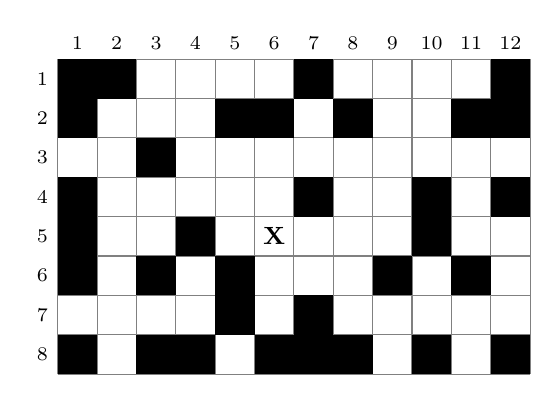
\begin{tikzpicture}[x=0.5cm, y=0.5cm]
						% Định nghĩa số hàng và số cột
						\def\rows{8}
						\def\cols{12}
						
						% Vẽ lưới ô vuông
						\draw[step=1, gray, thin] (1, -\rows) grid (\cols+1, 0);
						
						% Đánh số cột (1 -> 12)
						\foreach \c in {1,...,12} {
							\node[anchor=south, font=\scriptsize] at (\c + 0.5, 0) {\c};
						}
						
						% Đánh số hàng (1 -> 8)
						\foreach \r in {1,...,8} {
							\node[anchor=east, font=\scriptsize] at (1, -\r + 0.5) {\r};
						}
						
						% --- TÔ MÀU CÁC Ô TƯỜNG (MÀU ĐEN) ---
						\foreach \c/\r in {
							% Hàng 1
							1/1, 2/1, 7/1, 12/1,
							% Hàng 2
							1/2, 5/2, 6/2, 8/2, 11/2, 12/2,
							% Hàng 3
							3/3,
							% Hàng 4
							1/4, 7/4, 10/4, 12/4,
							% Hàng 5
							1/5, 4/5, 10/5,
							% Hàng 6
							1/6, 3/6, 5/6, 9/6, 11/6,
							% Hàng 7
							5/7, 7/7,
							% Hàng 8
							1/8, 4/8, 3/8, 6/8, 7/8, 8/8, 10/8, 12/8
						} {
							\fill[black] (\c, -\r) rectangle ++(1, 1);
						}
						
						% --- ĐIỂM XUẤT PHÁT X tại (6, 5) ---
						% Lưu ý: Tọa độ trong tikz là (cột, -hàng) nên (5,6) là cột 6, hàng 5
						\node[font=\bfseries\small] at (6.5, -4.5) {X};
						
					\end{tikzpicture}
				\end{adjustbox}
			\end{column}
		\end{columns}
	\end{frame}
	
	\begin{frame}[t]{Minh họa}
		\setlength{\leftmargini}{-0.5em}

		\begin{columns}[T]
			% --- CỘT TRÁI: TEXT VÀ QUEUE ---
			\begin{column}{0.5\textwidth}
				% Bullet point Minh họa
				\begin{itemize}
					\item \textbf{Minh họa}
				\end{itemize}
				\vspace{2.8cm} 
				
				% Nội dung thao tác
				\noindent \large Lấy (5,6) ra khỏi Q \\[0.2cm]
				\noindent \large Đưa trạng thái (5,7), (5, 5), (4, 6), (6,6) vào Q
	
				\begin{tabular}{|c|c|c|c|c|p{3.5cm}|}
					\hline
					\small (5,6) & \small (5,7) & \small (5,5) & \small (4,6) & \small (6,6) & ~ \\[0.1cm]
					\hline
				\end{tabular}
			\end{column}
			
			% --- CỘT PHẢI: MÊ CUNG ---
			\begin{column}{0.5\textwidth}
				\centering
				\begin{adjustbox}{width=0.9\linewidth}
					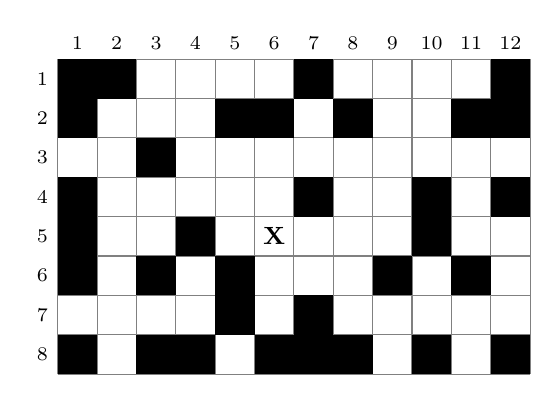
\begin{tikzpicture}[x=0.5cm, y=0.5cm]
						% Định nghĩa số hàng và số cột
						\def\rows{8}
						\def\cols{12}
						
						% Vẽ lưới ô vuông
						\draw[step=1, gray, thin] (1, -\rows) grid (\cols+1, 0);
						
						% Đánh số cột (1 -> 12)
						\foreach \c in {1,...,12} {
							\node[anchor=south, font=\scriptsize] at (\c + 0.5, 0) {\c};
						}
						
						% Đánh số hàng (1 -> 8)
						\foreach \r in {1,...,8} {
							\node[anchor=east, font=\scriptsize] at (1, -\r + 0.5) {\r};
						}
						
						% --- TÔ MÀU CÁC Ô TƯỜNG (MÀU ĐEN) - GIỮ NGUYÊN ---
						\foreach \c/\r in {
							1/1, 2/1, 7/1, 12/1,
							1/2, 5/2, 6/2, 8/2, 11/2, 12/2,
							3/3,
							1/4, 7/4, 10/4, 12/4,
							1/5, 4/5, 10/5,
							1/6, 3/6, 5/6, 9/6, 11/6,
							5/7, 7/7,
							1/8, 4/8, 3/8, 6/8, 7/8, 8/8, 10/8, 12/8
						} {
							\fill[black] (\c, -\r) rectangle ++(1, 1);
						}
						
						% --- ĐIỂM XUẤT PHÁT X TẠI (5,6) [Cột 6, Hàng 5] ---
						\node[font=\bfseries\small] at (6.5, -4.5) {X};
						
					\end{tikzpicture}
				\end{adjustbox}
			\end{column}
		\end{columns}
	\end{frame}
	
	\begin{frame}[t]{Minh họa}
		% Thay đổi lề theo yêu cầu
		\setlength{\leftmargini}{-0.5em}
		
		\vspace{0.2cm}
		\begin{columns}[T]
			% --- CỘT TRÁI: TEXT VÀ QUEUE ---
			\begin{column}{0.55\textwidth} % Tăng độ rộng cột trái một chút để bảng không bị chật
				\begin{itemize}
					\item \textbf{Minh họa}
				\end{itemize}
				
				% Khoảng trống lớn để đẩy nội dung xuống
				\vspace{3.2cm} 
				
				\noindent \large Lấy (5,7) ra khỏi Q \\[0.2cm]
				\noindent \large Đưa trạng thái (6,7), (5, 8) vào Q
				
				\vspace{0.3cm}
				
				% Vẽ bảng Queue có gạch chéo đỏ
				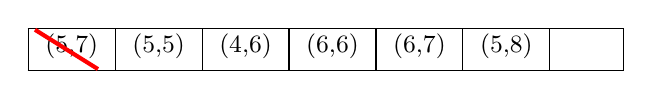
\begin{tikzpicture}
					\node[anchor=west, inner sep=0] (tbl) {
						\begin{tabular}{|c|c|c|c|c|c|p{0.5cm}|}
							\hline
							\small (5,7) & \small (5,5) & \small (4,6) & \small (6,6) & \small (6,7) & \small (5,8) & ~ \\[0.1cm]
							\hline
						\end{tabular}
					};
					% Vẽ đường gạch chéo đỏ lên ô đầu tiên
					% Tinh chỉnh toạ độ thủ công đè lên ô (5,7)
					\draw[red, line width=1.5pt] (0.1, 0.25) -- (0.9, -0.25);
				\end{tikzpicture}
			\end{column}
			
			% --- CỘT PHẢI: MÊ CUNG ---
			\begin{column}{0.45\textwidth}
				\centering
				\begin{adjustbox}{width=0.95\linewidth}
					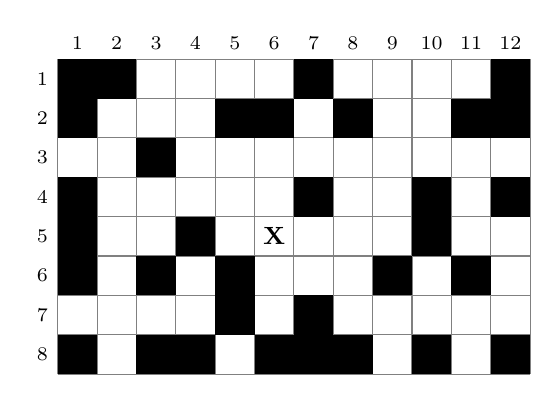
\begin{tikzpicture}[x=0.5cm, y=0.5cm]
						% Định nghĩa số hàng và số cột
						\def\rows{8}
						\def\cols{12}
						
						% Vẽ lưới ô vuông
						\draw[step=1, gray, thin] (1, -\rows) grid (\cols+1, 0);
						
						% Đánh số cột (1 -> 12)
						\foreach \c in {1,...,12} {
							\node[anchor=south, font=\scriptsize] at (\c + 0.5, 0) {\c};
						}
						
						% Đánh số hàng (1 -> 8)
						\foreach \r in {1,...,8} {
							\node[anchor=east, font=\scriptsize] at (1, -\r + 0.5) {\r};
						}
						
						% --- TÔ MÀU CÁC Ô TƯỜNG (MÀU ĐEN) ---
						\foreach \c/\r in {
							1/1, 2/1, 7/1, 12/1,
							1/2, 5/2, 6/2, 8/2, 11/2, 12/2,
							3/3,
							1/4, 7/4, 10/4, 12/4,
							1/5, 4/5, 10/5,
							1/6, 3/6, 5/6, 9/6, 11/6,
							5/7, 7/7,
							1/8, 4/8, 3/8, 6/8, 7/8, 8/8, 10/8, 12/8
						} {
							\fill[black] (\c, -\r) rectangle ++(1, 1);
						}
						
						% --- ĐIỂM XUẤT PHÁT X TẠI (5,6) ---
						\node[font=\bfseries\small] at (6.5, -4.5) {X};
						
					\end{tikzpicture}
				\end{adjustbox}
			\end{column}
		\end{columns}
	\end{frame}
	
	% --- SLIDE 61 ---
	\begin{frame}[t]{Minh họa}
		\setlength{\leftmargini}{-0.5em}
		\vspace{0.2cm}
		\begin{columns}[T]
			% CỘT TRÁI
			\begin{column}{0.55\textwidth}
				\begin{itemize} \item \textbf{Minh họa} \end{itemize}
				\vspace{3.2cm} 
				\noindent \large Lấy (5,5) ra khỏi Q \\[0.2cm]
				\noindent \large Đưa trạng thái (4,5) vào Q
				\vspace{0.3cm}
				% Hàng đợi
				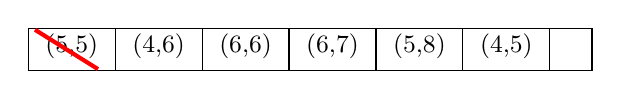
\begin{tikzpicture}
					\node[anchor=west, inner sep=0] (tbl) {
						\begin{tabular}{|c|c|c|c|c|c|p{0.1cm}|}
							\hline
							\small (5,5) & \small (4,6) & \small (6,6) & \small (6,7) & \small (5,8) & \small (4,5) & ~ \\[0.1cm]
							\hline
						\end{tabular}
					};
					\draw[red, line width=1.5pt] (0.1, 0.25) -- (0.9, -0.25);
				\end{tikzpicture}
			\end{column}
			% CỘT PHẢI (MÊ CUNG)
			\begin{column}{0.45\textwidth}
				\centering
				\begin{adjustbox}{width=0.95\linewidth}
					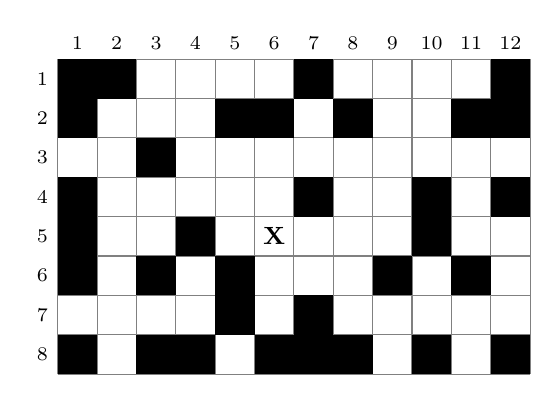
\begin{tikzpicture}[x=0.5cm, y=0.5cm]
						\def\rows{8} \def\cols{12}
						\draw[step=1, gray, thin] (1, -\rows) grid (\cols+1, 0);
						\foreach \c in {1,...,12} { \node[anchor=south, font=\scriptsize] at (\c + 0.5, 0) {\c}; }
						\foreach \r in {1,...,8} { \node[anchor=east, font=\scriptsize] at (1, -\r + 0.5) {\r}; }
						\foreach \c/\r in { 1/1, 2/1, 7/1, 12/1, 1/2, 5/2, 6/2, 8/2, 11/2, 12/2, 3/3, 1/4, 7/4, 10/4, 12/4, 1/5, 4/5, 10/5, 1/6, 3/6, 5/6, 9/6, 11/6, 5/7, 7/7, 1/8, 4/8, 3/8, 6/8, 7/8, 8/8, 10/8, 12/8 } { \fill[black] (\c, -\r) rectangle ++(1, 1); }
						\node[font=\bfseries\small] at (6.5, -4.5) {X};
					\end{tikzpicture}
				\end{adjustbox}
			\end{column}
		\end{columns}
	\end{frame}
	
	% --- SLIDE 62 ---
	\begin{frame}[t]{Minh họa}
		\setlength{\leftmargini}{-0.5em}
		\vspace{0.2cm}
		\begin{columns}[T]
			\begin{column}{0.55\textwidth}
				\begin{itemize} \item \textbf{Minh họa} \end{itemize}
				\vspace{3.2cm} 
				\noindent \large Lấy (4,6) ra khỏi Q \\[0.2cm]
				\noindent \large Đưa trạng thái (3,6) vào Q
				\vspace{0.3cm}
				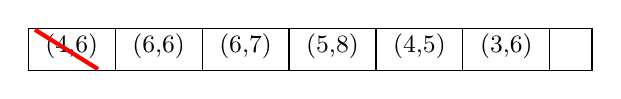
\begin{tikzpicture}
					\node[anchor=west, inner sep=0] (tbl) {
						\begin{tabular}{|c|c|c|c|c|c|p{0.1cm}|}
							\hline
							\small (4,6) & \small (6,6) & \small (6,7) & \small (5,8) & \small (4,5) & \small (3,6) & ~ \\[0.1cm]
							\hline
						\end{tabular}
					};
					\draw[red, line width=1.5pt] (0.1, 0.25) -- (0.9, -0.25);
				\end{tikzpicture}
			\end{column}
			\begin{column}{0.45\textwidth}
				\centering
				\begin{adjustbox}{width=0.95\linewidth}
					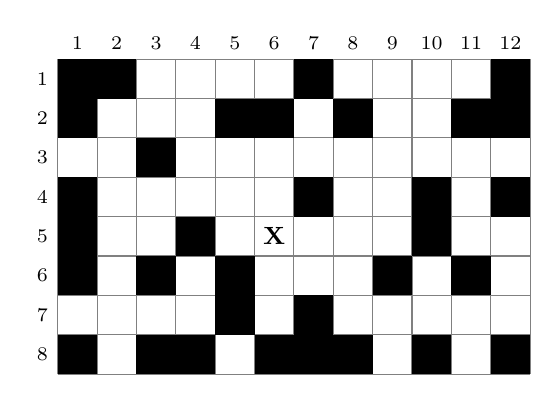
\begin{tikzpicture}[x=0.5cm, y=0.5cm]
						\def\rows{8} \def\cols{12}
						\draw[step=1, gray, thin] (1, -\rows) grid (\cols+1, 0);
						\foreach \c in {1,...,12} { \node[anchor=south, font=\scriptsize] at (\c + 0.5, 0) {\c}; }
						\foreach \r in {1,...,8} { \node[anchor=east, font=\scriptsize] at (1, -\r + 0.5) {\r}; }
						\foreach \c/\r in { 1/1, 2/1, 7/1, 12/1, 1/2, 5/2, 6/2, 8/2, 11/2, 12/2, 3/3, 1/4, 7/4, 10/4, 12/4, 1/5, 4/5, 10/5, 1/6, 3/6, 5/6, 9/6, 11/6, 5/7, 7/7, 1/8, 4/8, 3/8, 6/8, 7/8, 8/8, 10/8, 12/8 } { \fill[black] (\c, -\r) rectangle ++(1, 1); }
						\node[font=\bfseries\small] at (6.5, -4.5) {X};
					\end{tikzpicture}
				\end{adjustbox}
			\end{column}
		\end{columns}
	\end{frame}
	
	% --- SLIDE 63 ---
	\begin{frame}[t]{Minh họa}
		\setlength{\leftmargini}{-0.5em}
		\vspace{0.2cm}
		\begin{columns}[T]
			\begin{column}{0.55\textwidth}
				\begin{itemize} \item \textbf{Minh họa} \end{itemize}
				\vspace{3.2cm} 
				\noindent \large Lấy (6,6) ra khỏi Q \\[0.2cm]
				\noindent \large Đưa trạng thái (7,6) vào Q
				\vspace{0.3cm}
				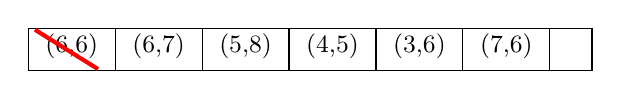
\begin{tikzpicture}
					\node[anchor=west, inner sep=0] (tbl) {
						\begin{tabular}{|c|c|c|c|c|c|p{0.1cm}|}
							\hline
							\small (6,6) & \small (6,7) & \small (5,8) & \small (4,5) & \small (3,6) & \small (7,6) & ~ \\[0.1cm]
							\hline
						\end{tabular}
					};
					\draw[red, line width=1.5pt] (0.1, 0.25) -- (0.9, -0.25);
				\end{tikzpicture}
			\end{column}
			\begin{column}{0.45\textwidth}
				\centering
				\begin{adjustbox}{width=0.95\linewidth}
					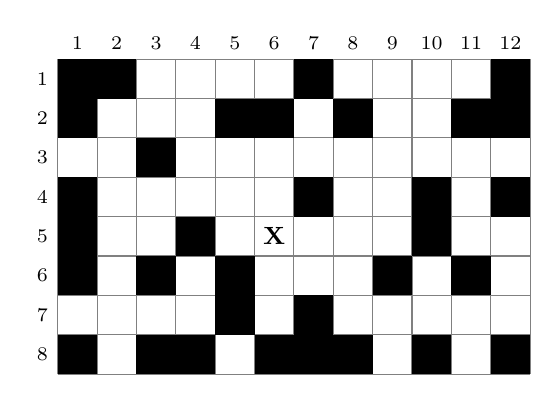
\begin{tikzpicture}[x=0.5cm, y=0.5cm]
						\def\rows{8} \def\cols{12}
						\draw[step=1, gray, thin] (1, -\rows) grid (\cols+1, 0);
						\foreach \c in {1,...,12} { \node[anchor=south, font=\scriptsize] at (\c + 0.5, 0) {\c}; }
						\foreach \r in {1,...,8} { \node[anchor=east, font=\scriptsize] at (1, -\r + 0.5) {\r}; }
						\foreach \c/\r in { 1/1, 2/1, 7/1, 12/1, 1/2, 5/2, 6/2, 8/2, 11/2, 12/2, 3/3, 1/4, 7/4, 10/4, 12/4, 1/5, 4/5, 10/5, 1/6, 3/6, 5/6, 9/6, 11/6, 5/7, 7/7, 1/8, 4/8, 3/8, 6/8, 7/8, 8/8, 10/8, 12/8 } { \fill[black] (\c, -\r) rectangle ++(1, 1); }
						\node[font=\bfseries\small] at (6.5, -4.5) {X};
					\end{tikzpicture}
				\end{adjustbox}
			\end{column}
		\end{columns}
	\end{frame}
	
	% --- SLIDE 64 ---
	\begin{frame}[t]{Minh họa}
		\setlength{\leftmargini}{-0.5em}
		\vspace{0.2cm}
		\begin{columns}[T]
			\begin{column}{0.55\textwidth}
				\begin{itemize} \item \textbf{Minh họa} \end{itemize}
				\vspace{3.2cm} 
				\noindent \large Lấy (6,7) ra khỏi Q \\[0.2cm]
				\noindent \large Đưa trạng thái (6,8) vào Q
				\vspace{0.3cm}
				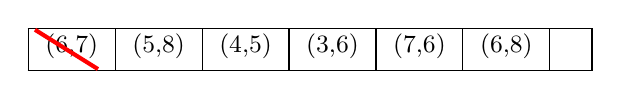
\begin{tikzpicture}
					\node[anchor=west, inner sep=0] (tbl) {
						\begin{tabular}{|c|c|c|c|c|c|p{0.1cm}|}
							\hline
							\small (6,7) & \small (5,8) & \small (4,5) & \small (3,6) & \small (7,6) & \small (6,8) & ~ \\[0.1cm]
							\hline
						\end{tabular}
					};
					\draw[red, line width=1.5pt] (0.1, 0.25) -- (0.9, -0.25);
				\end{tikzpicture}
			\end{column}
			\begin{column}{0.45\textwidth}
				\centering
				\begin{adjustbox}{width=0.95\linewidth}
					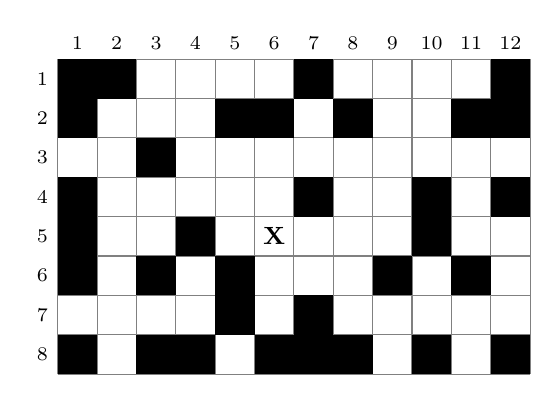
\begin{tikzpicture}[x=0.5cm, y=0.5cm]
						\def\rows{8} \def\cols{12}
						\draw[step=1, gray, thin] (1, -\rows) grid (\cols+1, 0);
						\foreach \c in {1,...,12} { \node[anchor=south, font=\scriptsize] at (\c + 0.5, 0) {\c}; }
						\foreach \r in {1,...,8} { \node[anchor=east, font=\scriptsize] at (1, -\r + 0.5) {\r}; }
						\foreach \c/\r in { 1/1, 2/1, 7/1, 12/1, 1/2, 5/2, 6/2, 8/2, 11/2, 12/2, 3/3, 1/4, 7/4, 10/4, 12/4, 1/5, 4/5, 10/5, 1/6, 3/6, 5/6, 9/6, 11/6, 5/7, 7/7, 1/8, 4/8, 3/8, 6/8, 7/8, 8/8, 10/8, 12/8 } { \fill[black] (\c, -\r) rectangle ++(1, 1); }
						\node[font=\bfseries\small] at (6.5, -4.5) {X};
					\end{tikzpicture}
				\end{adjustbox}
			\end{column}
		\end{columns}
	\end{frame}
	
	% --- SLIDE 65 ---
	\begin{frame}[t]{Minh họa}
		\setlength{\leftmargini}{-0.5em}
		\vspace{0.2cm}
		\begin{columns}[T]
			\begin{column}{0.55\textwidth}
				\begin{itemize} \item \textbf{Minh họa} \end{itemize}
				\vspace{3.2cm} 
				\noindent \large Lấy (5,8) ra khỏi Q \\[0.2cm]
				\noindent \large Đưa trạng thái (5,9) và(4,8) vào Q
				\vspace{0.3cm}
				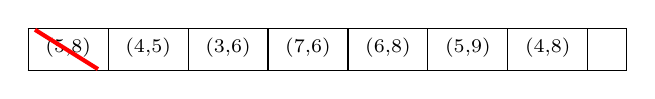
\begin{tikzpicture}
					\node[anchor=west, inner sep=0] (tbl) {
						% Slide này hàng đợi dài hơn nên dùng scriptsize
						\begin{tabular}{|c|c|c|c|c|c|c|p{0.05cm}|}
							\hline
							\scriptsize (5,8) & \scriptsize (4,5) & \scriptsize (3,6) & \scriptsize (7,6) & \scriptsize (6,8) & \scriptsize (5,9) & \scriptsize (4,8) & ~ \\[0.1cm]
							\hline
						\end{tabular}
					};
					\draw[red, line width=1.5pt] (0.1, 0.25) -- (0.9, -0.25);
				\end{tikzpicture}
			\end{column}
			\begin{column}{0.45\textwidth}
				\centering
				\begin{adjustbox}{width=0.95\linewidth}
					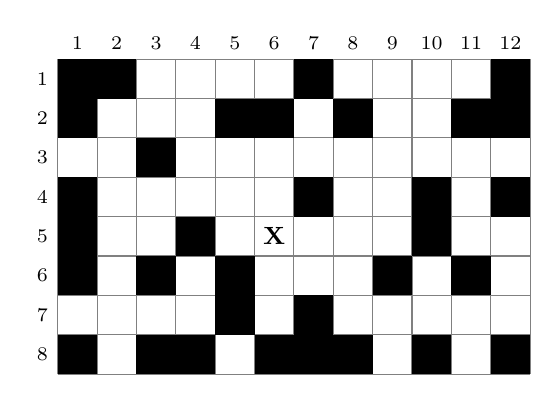
\begin{tikzpicture}[x=0.5cm, y=0.5cm]
						\def\rows{8} \def\cols{12}
						\draw[step=1, gray, thin] (1, -\rows) grid (\cols+1, 0);
						\foreach \c in {1,...,12} { \node[anchor=south, font=\scriptsize] at (\c + 0.5, 0) {\c}; }
						\foreach \r in {1,...,8} { \node[anchor=east, font=\scriptsize] at (1, -\r + 0.5) {\r}; }
						\foreach \c/\r in { 1/1, 2/1, 7/1, 12/1, 1/2, 5/2, 6/2, 8/2, 11/2, 12/2, 3/3, 1/4, 7/4, 10/4, 12/4, 1/5, 4/5, 10/5, 1/6, 3/6, 5/6, 9/6, 11/6, 5/7, 7/7, 1/8, 4/8, 3/8, 6/8, 7/8, 8/8, 10/8, 12/8 } { \fill[black] (\c, -\r) rectangle ++(1, 1); }
						\node[font=\bfseries\small] at (6.5, -4.5) {X};
					\end{tikzpicture}
				\end{adjustbox}
			\end{column}
		\end{columns}
	\end{frame}
	
	% --- SLIDE 66 ---
	\begin{frame}[t]{Minh họa}
		\setlength{\leftmargini}{-0.5em}
		\vspace{0.2cm}
		\begin{columns}[T]
			% CỘT TRÁI
			\begin{column}{0.55\textwidth}
				\begin{itemize} \item \textbf{Minh họa} \end{itemize}
				\vspace{3.2cm} 
				\noindent \large Lấy (4,5) ra khỏi Q \\[0.2cm]
				\noindent \large Đưa trạng thái (4,4) và(3,5) vào Q
				\vspace{0.3cm}
				% Hàng đợi dài -> dùng scriptsize
				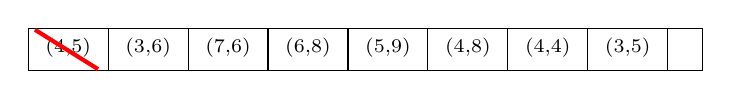
\begin{tikzpicture}
					\node[anchor=west, inner sep=0] (tbl) {
						\begin{tabular}{|c|c|c|c|c|c|c|c|p{0.01cm}|}
							\hline
							\scriptsize (4,5) & \scriptsize (3,6) & \scriptsize (7,6) & \scriptsize (6,8) & \scriptsize (5,9) & \scriptsize (4,8) & \scriptsize (4,4) & \scriptsize (3,5) & ~ \\[0.1cm]
							\hline
						\end{tabular}
					};
					\draw[red, line width=1.5pt] (0.1, 0.25) -- (0.9, -0.25);
				\end{tikzpicture}
			\end{column}
			% CỘT PHẢI (MÊ CUNG)
			\begin{column}{0.45\textwidth}
				\centering
				\begin{adjustbox}{width=0.95\linewidth}
					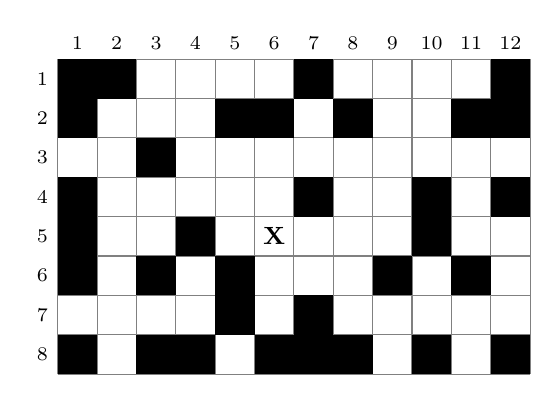
\begin{tikzpicture}[x=0.5cm, y=0.5cm]
						\def\rows{8} \def\cols{12}
						\draw[step=1, gray, thin] (1, -\rows) grid (\cols+1, 0);
						\foreach \c in {1,...,12} { \node[anchor=south, font=\scriptsize] at (\c + 0.5, 0) {\c}; }
						\foreach \r in {1,...,8} { \node[anchor=east, font=\scriptsize] at (1, -\r + 0.5) {\r}; }
						\foreach \c/\r in { 1/1, 2/1, 7/1, 12/1, 1/2, 5/2, 6/2, 8/2, 11/2, 12/2, 3/3, 1/4, 7/4, 10/4, 12/4, 1/5, 4/5, 10/5, 1/6, 3/6, 5/6, 9/6, 11/6, 5/7, 7/7, 1/8, 4/8, 3/8, 6/8, 7/8, 8/8, 10/8, 12/8 } { \fill[black] (\c, -\r) rectangle ++(1, 1); }
						\node[font=\bfseries\small] at (6.5, -4.5) {X};
					\end{tikzpicture}
				\end{adjustbox}
			\end{column}
		\end{columns}
	\end{frame}
	
	% --- SLIDE 67 ---
	\begin{frame}[t]{Minh họa}
		\setlength{\leftmargini}{-0.5em}
		\vspace{0.2cm}
		\begin{columns}[T]
			\begin{column}{0.55\textwidth}
				\begin{itemize} \item \textbf{Minh họa} \end{itemize}
				\vspace{3.2cm} 
				\noindent \large Lấy (3,6) ra khỏi Q \\[0.2cm]
				\noindent \large Đưa trạng thái (3,7) vào Q
				\vspace{0.3cm}
				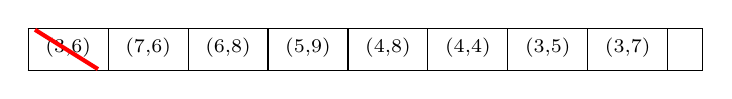
\begin{tikzpicture}
					\node[anchor=west, inner sep=0] (tbl) {
						\begin{tabular}{|c|c|c|c|c|c|c|c|p{0.01cm}|}
							\hline
							\scriptsize (3,6) & \scriptsize (7,6) & \scriptsize (6,8) & \scriptsize (5,9) & \scriptsize (4,8) & \scriptsize (4,4) & \scriptsize (3,5) & \scriptsize (3,7) & ~ \\[0.1cm]
							\hline
						\end{tabular}
					};
					\draw[red, line width=1.5pt] (0.1, 0.25) -- (0.9, -0.25);
				\end{tikzpicture}
			\end{column}
			\begin{column}{0.45\textwidth}
				\centering
				\begin{adjustbox}{width=0.95\linewidth}
					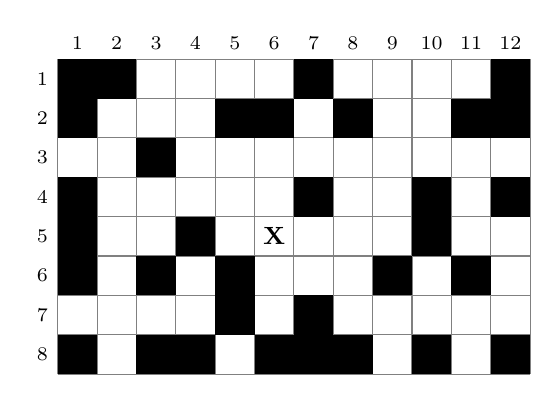
\begin{tikzpicture}[x=0.5cm, y=0.5cm]
						\def\rows{8} \def\cols{12}
						\draw[step=1, gray, thin] (1, -\rows) grid (\cols+1, 0);
						\foreach \c in {1,...,12} { \node[anchor=south, font=\scriptsize] at (\c + 0.5, 0) {\c}; }
						\foreach \r in {1,...,8} { \node[anchor=east, font=\scriptsize] at (1, -\r + 0.5) {\r}; }
						\foreach \c/\r in { 1/1, 2/1, 7/1, 12/1, 1/2, 5/2, 6/2, 8/2, 11/2, 12/2, 3/3, 1/4, 7/4, 10/4, 12/4, 1/5, 4/5, 10/5, 1/6, 3/6, 5/6, 9/6, 11/6, 5/7, 7/7, 1/8, 4/8, 3/8, 6/8, 7/8, 8/8, 10/8, 12/8 } { \fill[black] (\c, -\r) rectangle ++(1, 1); }
						\node[font=\bfseries\small] at (6.5, -4.5) {X};
					\end{tikzpicture}
				\end{adjustbox}
			\end{column}
		\end{columns}
	\end{frame}
	
	% --- SLIDE 68 ---
	\begin{frame}[t]{Minh họa}
		\setlength{\leftmargini}{-0.5em}
		\vspace{0.2cm}
		\begin{columns}[T]
			\begin{column}{0.55\textwidth}
				\begin{itemize} \item \textbf{Minh họa} \end{itemize}
				\vspace{3.2cm} 
				\noindent \large Lấy (7,6) ra khỏi Q \\[0.2cm]
				\noindent \large Không đưa được trạng thái mới nào vào Q
				\vspace{0.3cm}
				\begin{tikzpicture}
					\node[anchor=west, inner sep=0] (tbl) {
						\begin{tabular}{|c|c|c|c|c|c|c|p{0.01cm}|}
							\hline
							\scriptsize (7,6) & \scriptsize (6,8) & \scriptsize (5,9) & \scriptsize (4,8) & \scriptsize (4,4) & \scriptsize (3,5) & \scriptsize (3,7) & ~ \\[0.1cm]
							\hline
						\end{tabular}
					};
					\draw[red, line width=1.5pt] (0.1, 0.25) -- (0.9, -0.25);
				\end{tikzpicture}
			\end{column}
			\begin{column}{0.45\textwidth}
				\centering
				\begin{adjustbox}{width=0.95\linewidth}
					\begin{tikzpicture}[x=0.5cm, y=0.5cm]
						\def\rows{8} \def\cols{12}
						\draw[step=1, gray, thin] (1, -\rows) grid (\cols+1, 0);
						\foreach \c in {1,...,12} { \node[anchor=south, font=\scriptsize] at (\c + 0.5, 0) {\c}; }
						\foreach \r in {1,...,8} { \node[anchor=east, font=\scriptsize] at (1, -\r + 0.5) {\r}; }
						\foreach \c/\r in { 1/1, 2/1, 7/1, 12/1, 1/2, 5/2, 6/2, 8/2, 11/2, 12/2, 3/3, 1/4, 7/4, 10/4, 12/4, 1/5, 4/5, 10/5, 1/6, 3/6, 5/6, 9/6, 11/6, 5/7, 7/7, 1/8, 4/8, 3/8, 6/8, 7/8, 8/8, 10/8, 12/8 } { \fill[black] (\c, -\r) rectangle ++(1, 1); }
						\node[font=\bfseries\small] at (6.5, -4.5) {X};
					\end{tikzpicture}
				\end{adjustbox}
			\end{column}
		\end{columns}
	\end{frame}
	
	% --- SLIDE 69 ---
	\begin{frame}[t]{Minh họa}
		\setlength{\leftmargini}{-0.5em}
		\vspace{0.2cm}
		\begin{columns}[T]
			\begin{column}{0.55\textwidth}
				\begin{itemize} \item \textbf{Minh họa} \end{itemize}
				\vspace{3.2cm} 
				\noindent \large Lấy (6,8) ra khỏi Q \\[0.2cm]
				\noindent \large Đưa được trạng thái (7,8) vào Q
				\vspace{0.3cm}
				\begin{tikzpicture}
					\node[anchor=west, inner sep=0] (tbl) {
						\begin{tabular}{|c|c|c|c|c|c|c|p{0.01cm}|}
							\hline
							\scriptsize (6,8) & \scriptsize (5,9) & \scriptsize (4,8) & \scriptsize (4,4) & \scriptsize (3,5) & \scriptsize (3,7) & \scriptsize (7,8) & ~ \\[0.1cm]
							\hline
						\end{tabular}
					};
					\draw[red, line width=1.5pt] (0.1, 0.25) -- (0.9, -0.25);
				\end{tikzpicture}
			\end{column}
			\begin{column}{0.45\textwidth}
				\centering
				\begin{adjustbox}{width=0.95\linewidth}
					\begin{tikzpicture}[x=0.5cm, y=0.5cm]
						\def\rows{8} \def\cols{12}
						\draw[step=1, gray, thin] (1, -\rows) grid (\cols+1, 0);
						\foreach \c in {1,...,12} { \node[anchor=south, font=\scriptsize] at (\c + 0.5, 0) {\c}; }
						\foreach \r in {1,...,8} { \node[anchor=east, font=\scriptsize] at (1, -\r + 0.5) {\r}; }
						\foreach \c/\r in { 1/1, 2/1, 7/1, 12/1, 1/2, 5/2, 6/2, 8/2, 11/2, 12/2, 3/3, 1/4, 7/4, 10/4, 12/4, 1/5, 4/5, 10/5, 1/6, 3/6, 5/6, 9/6, 11/6, 5/7, 7/7, 1/8, 4/8, 3/8, 6/8, 7/8, 8/8, 10/8, 12/8 } { \fill[black] (\c, -\r) rectangle ++(1, 1); }
						\node[font=\bfseries\small] at (6.5, -4.5) {X};
					\end{tikzpicture}
				\end{adjustbox}
			\end{column}
		\end{columns}
	\end{frame}
	
	% --- SLIDE 70 ---
	\begin{frame}[t]{Minh họa}
		\setlength{\leftmargini}{-0.5em}
		\vspace{0.2cm}
		\begin{columns}[T]
			\begin{column}{0.55\textwidth}
				\begin{itemize} \item \textbf{Minh họa} \end{itemize}
				\vspace{3.2cm} 
				\noindent \large Lấy (5,9) ra khỏi Q \\[0.2cm]
				\noindent \large Đưa được trạng thái (4,9) vào Q
				\vspace{0.3cm}
				\begin{tikzpicture}
					\node[anchor=west, inner sep=0] (tbl) {
						\begin{tabular}{|c|c|c|c|c|c|c|p{0.01cm}|}
							\hline
							\scriptsize (5,9) & \scriptsize (4,8) & \scriptsize (4,4) & \scriptsize (3,5) & \scriptsize (3,7) & \scriptsize (7,8) & \scriptsize (4,9) & ~ \\[0.1cm]
							\hline
						\end{tabular}
					};
					\draw[red, line width=1.5pt] (0.1, 0.25) -- (0.9, -0.25);
				\end{tikzpicture}
			\end{column}
			\begin{column}{0.45\textwidth}
				\centering
				\begin{adjustbox}{width=0.95\linewidth}
					\begin{tikzpicture}[x=0.5cm, y=0.5cm]
						\def\rows{8} \def\cols{12}
						\draw[step=1, gray, thin] (1, -\rows) grid (\cols+1, 0);
						\foreach \c in {1,...,12} { \node[anchor=south, font=\scriptsize] at (\c + 0.5, 0) {\c}; }
						\foreach \r in {1,...,8} { \node[anchor=east, font=\scriptsize] at (1, -\r + 0.5) {\r}; }
						\foreach \c/\r in { 1/1, 2/1, 7/1, 12/1, 1/2, 5/2, 6/2, 8/2, 11/2, 12/2, 3/3, 1/4, 7/4, 10/4, 12/4, 1/5, 4/5, 10/5, 1/6, 3/6, 5/6, 9/6, 11/6, 5/7, 7/7, 1/8, 4/8, 3/8, 6/8, 7/8, 8/8, 10/8, 12/8 } { \fill[black] (\c, -\r) rectangle ++(1, 1); }
						\node[font=\bfseries\small] at (6.5, -4.5) {X};
					\end{tikzpicture}
				\end{adjustbox}
			\end{column}
		\end{columns}
	\end{frame}
	
	% --- SLIDE 71 ---
	\begin{frame}[t]{Minh họa}
		\setlength{\leftmargini}{-0.5em}
		\vspace{0.2cm}
		\begin{columns}[T]
			\begin{column}{0.55\textwidth}
				\begin{itemize} \item \textbf{Minh họa} \end{itemize}
				\vspace{3.2cm} 
				\noindent \large Lấy (4,8) ra khỏi Q \\[0.2cm]
				\noindent \large Đưa được trạng thái (3,8) vào Q
				\vspace{0.3cm}
				\begin{tikzpicture}
					\node[anchor=west, inner sep=0] (tbl) {
						\begin{tabular}{|c|c|c|c|c|c|c|p{0.01cm}|}
							\hline
							\scriptsize (4,8) & \scriptsize (4,4) & \scriptsize (3,5) & \scriptsize (3,7) & \scriptsize (7,8) & \scriptsize (4,9) & \scriptsize (3,8) & ~ \\[0.1cm]
							\hline
						\end{tabular}
					};
					\draw[red, line width=1.5pt] (0.1, 0.25) -- (0.9, -0.25);
				\end{tikzpicture}
			\end{column}
			\begin{column}{0.45\textwidth}
				\centering
				\begin{adjustbox}{width=0.95\linewidth}
					\begin{tikzpicture}[x=0.5cm, y=0.5cm]
						\def\rows{8} \def\cols{12}
						\draw[step=1, gray, thin] (1, -\rows) grid (\cols+1, 0);
						\foreach \c in {1,...,12} { \node[anchor=south, font=\scriptsize] at (\c + 0.5, 0) {\c}; }
						\foreach \r in {1,...,8} { \node[anchor=east, font=\scriptsize] at (1, -\r + 0.5) {\r}; }
						\foreach \c/\r in { 1/1, 2/1, 7/1, 12/1, 1/2, 5/2, 6/2, 8/2, 11/2, 12/2, 3/3, 1/4, 7/4, 10/4, 12/4, 1/5, 4/5, 10/5, 1/6, 3/6, 5/6, 9/6, 11/6, 5/7, 7/7, 1/8, 4/8, 3/8, 6/8, 7/8, 8/8, 10/8, 12/8 } { \fill[black] (\c, -\r) rectangle ++(1, 1); }
						\node[font=\bfseries\small] at (6.5, -4.5) {X};
					\end{tikzpicture}
				\end{adjustbox}
			\end{column}
		\end{columns}
	\end{frame}
	
	% --- SLIDE 72 ---
	\begin{frame}[t]{Minh họa}
		\setlength{\leftmargini}{-0.5em}
		\vspace{0.2cm}
		\begin{columns}[T]
			\begin{column}{0.55\textwidth}
				\begin{itemize} \item \textbf{Minh họa} \end{itemize}
				\vspace{3.2cm} 
				\noindent \large Lấy (4,4) ra khỏi Q \\[0.2cm]
				\noindent \large Đưa được trạng thái (4,3), (3,4) vào Q
				\vspace{0.3cm}
				\begin{tikzpicture}
					\node[anchor=west, inner sep=0] (tbl) {
						\begin{tabular}{|c|c|c|c|c|c|c|c|p{0.01cm}|}
							\hline
							\scriptsize (4,4) & \scriptsize (3,5) & \scriptsize (3,7) & \scriptsize (7,8) & \scriptsize (4,9) & \scriptsize (3,8) & \scriptsize (4,3) & \scriptsize (3,4) & ~ \\[0.1cm]
							\hline
						\end{tabular}
					};
					\draw[red, line width=1.5pt] (0.1, 0.25) -- (0.9, -0.25);
				\end{tikzpicture}
			\end{column}
			\begin{column}{0.45\textwidth}
				\centering
				\begin{adjustbox}{width=0.95\linewidth}
					\begin{tikzpicture}[x=0.5cm, y=0.5cm]
						\def\rows{8} \def\cols{12}
						\draw[step=1, gray, thin] (1, -\rows) grid (\cols+1, 0);
						\foreach \c in {1,...,12} { \node[anchor=south, font=\scriptsize] at (\c + 0.5, 0) {\c}; }
						\foreach \r in {1,...,8} { \node[anchor=east, font=\scriptsize] at (1, -\r + 0.5) {\r}; }
						\foreach \c/\r in { 1/1, 2/1, 7/1, 12/1, 1/2, 5/2, 6/2, 8/2, 11/2, 12/2, 3/3, 1/4, 7/4, 10/4, 12/4, 1/5, 4/5, 10/5, 1/6, 3/6, 5/6, 9/6, 11/6, 5/7, 7/7, 1/8, 4/8, 3/8, 6/8, 7/8, 8/8, 10/8, 12/8 } { \fill[black] (\c, -\r) rectangle ++(1, 1); }
						\node[font=\bfseries\small] at (6.5, -4.5) {X};
					\end{tikzpicture}
				\end{adjustbox}
			\end{column}
		\end{columns}
	\end{frame}
	
	% --- SLIDE 73 ---
	\begin{frame}[t]{Minh họa}
		\setlength{\leftmargini}{-0.5em}
		\vspace{0.2cm}
		\begin{columns}[T]
			\begin{column}{0.55\textwidth}
				\begin{itemize} \item \textbf{Minh họa} \end{itemize}
				\vspace{3.2cm} 
				\noindent \large Lấy (3,5) ra khỏi Q \\[0.2cm]
				\noindent \large Không đưa được trạng thái mới nào vào Q
				\vspace{0.3cm}
				\begin{tikzpicture}
					\node[anchor=west, inner sep=0] (tbl) {
						\begin{tabular}{|c|c|c|c|c|c|p{0.01cm}|}
							\hline
							\scriptsize (3,5) & \scriptsize (3,7) & \scriptsize (7,8) & \scriptsize (4,9) & \scriptsize (3,8) & \scriptsize (4,3) & ~ \\[0.1cm]
							\hline
						\end{tabular}
					};
					\draw[red, line width=1.5pt] (0.1, 0.25) -- (0.9, -0.25);
				\end{tikzpicture}
			\end{column}
			\begin{column}{0.45\textwidth}
				\centering
				\begin{adjustbox}{width=0.95\linewidth}
					\begin{tikzpicture}[x=0.5cm, y=0.5cm]
						\def\rows{8} \def\cols{12}
						\draw[step=1, gray, thin] (1, -\rows) grid (\cols+1, 0);
						\foreach \c in {1,...,12} { \node[anchor=south, font=\scriptsize] at (\c + 0.5, 0) {\c}; }
						\foreach \r in {1,...,8} { \node[anchor=east, font=\scriptsize] at (1, -\r + 0.5) {\r}; }
						\foreach \c/\r in { 1/1, 2/1, 7/1, 12/1, 1/2, 5/2, 6/2, 8/2, 11/2, 12/2, 3/3, 1/4, 7/4, 10/4, 12/4, 1/5, 4/5, 10/5, 1/6, 3/6, 5/6, 9/6, 11/6, 5/7, 7/7, 1/8, 4/8, 3/8, 6/8, 7/8, 8/8, 10/8, 12/8 } { \fill[black] (\c, -\r) rectangle ++(1, 1); }
						\node[font=\bfseries\small] at (6.5, -4.5) {X};
					\end{tikzpicture}
				\end{adjustbox}
			\end{column}
		\end{columns}
	\end{frame}
	
	% --- SLIDE 74 ---
	\begin{frame}[t]{Minh họa}
		\setlength{\leftmargini}{-0.5em}
		\vspace{0.2cm}
		\begin{columns}[T]
			\begin{column}{0.55\textwidth}
				\begin{itemize} \item \textbf{Minh họa} \end{itemize}
				\vspace{3.2cm} 
				\noindent \large Lấy (3,7) ra khỏi Q \\[0.2cm]
				\noindent \large Đưa được trạng thái mới (2,7) vào Q
				\vspace{0.3cm}
				\begin{tikzpicture}
					\node[anchor=west, inner sep=0] (tbl) {
						\begin{tabular}{|c|c|c|c|c|c|c|p{0.01cm}|}
							\hline
							\scriptsize (3,7) & \scriptsize (7,8) & \scriptsize (4,9) & \scriptsize (3,8) & \scriptsize (4,3) & \scriptsize (3,4) & \scriptsize (2,7) & ~ \\[0.1cm]
							\hline
						\end{tabular}
					};
					\draw[red, line width=1.5pt] (0.1, 0.25) -- (0.9, -0.25);
				\end{tikzpicture}
			\end{column}
			\begin{column}{0.45\textwidth}
				\centering
				\begin{adjustbox}{width=0.95\linewidth}
					\begin{tikzpicture}[x=0.5cm, y=0.5cm]
						\def\rows{8} \def\cols{12}
						\draw[step=1, gray, thin] (1, -\rows) grid (\cols+1, 0);
						\foreach \c in {1,...,12} { \node[anchor=south, font=\scriptsize] at (\c + 0.5, 0) {\c}; }
						\foreach \r in {1,...,8} { \node[anchor=east, font=\scriptsize] at (1, -\r + 0.5) {\r}; }
						\foreach \c/\r in { 1/1, 2/1, 7/1, 12/1, 1/2, 5/2, 6/2, 8/2, 11/2, 12/2, 3/3, 1/4, 7/4, 10/4, 12/4, 1/5, 4/5, 10/5, 1/6, 3/6, 5/6, 9/6, 11/6, 5/7, 7/7, 1/8, 4/8, 3/8, 6/8, 7/8, 8/8, 10/8, 12/8 } { \fill[black] (\c, -\r) rectangle ++(1, 1); }
						\node[font=\bfseries\small] at (6.5, -4.5) {X};
					\end{tikzpicture}
				\end{adjustbox}
			\end{column}
		\end{columns}
	\end{frame}
	
	% --- SLIDE 75 ---
	\begin{frame}[t]{Minh họa}
		\setlength{\leftmargini}{-0.5em}
		\vspace{0.2cm}
		\begin{columns}[T]
			\begin{column}{0.55\textwidth}
				\begin{itemize} \item \textbf{Minh họa} \end{itemize}
				\vspace{3.2cm} 
				\noindent \large Lấy (7,8) ra khỏi Q \\[0.2cm]
				\noindent \large Đưa được trạng thái mới (7,9) vào Q
				\vspace{0.3cm}
				\begin{tikzpicture}
					\node[anchor=west, inner sep=0] (tbl) {
						\begin{tabular}{|c|c|c|c|c|c|c|p{0.01cm}|}
							\hline
							\scriptsize (7,8) & \scriptsize (4,9) & \scriptsize (3,8) & \scriptsize (4,3) & \scriptsize (3,4) & \scriptsize (2,7) & \scriptsize (7,9) & ~ \\[0.1cm]
							\hline
						\end{tabular}
					};
					\draw[red, line width=1.5pt] (0.1, 0.25) -- (0.9, -0.25);
				\end{tikzpicture}
			\end{column}
			\begin{column}{0.45\textwidth}
				\centering
				\begin{adjustbox}{width=0.95\linewidth}
					\begin{tikzpicture}[x=0.5cm, y=0.5cm]
						\def\rows{8} \def\cols{12}
						\draw[step=1, gray, thin] (1, -\rows) grid (\cols+1, 0);
						\foreach \c in {1,...,12} { \node[anchor=south, font=\scriptsize] at (\c + 0.5, 0) {\c}; }
						\foreach \r in {1,...,8} { \node[anchor=east, font=\scriptsize] at (1, -\r + 0.5) {\r}; }
						\foreach \c/\r in { 1/1, 2/1, 7/1, 12/1, 1/2, 5/2, 6/2, 8/2, 11/2, 12/2, 3/3, 1/4, 7/4, 10/4, 12/4, 1/5, 4/5, 10/5, 1/6, 3/6, 5/6, 9/6, 11/6, 5/7, 7/7, 1/8, 4/8, 3/8, 6/8, 7/8, 8/8, 10/8, 12/8 } { \fill[black] (\c, -\r) rectangle ++(1, 1); }
						\node[font=\bfseries\small] at (6.5, -4.5) {X};
					\end{tikzpicture}
				\end{adjustbox}
			\end{column}
		\end{columns}
	\end{frame}
	
	% --- SLIDE 76 ---
	\begin{frame}[t]{Minh họa}
		\setlength{\leftmargini}{-0.5em}
		\vspace{0.2cm}
		\begin{columns}[T]
			\begin{column}{0.55\textwidth}
				\begin{itemize} \item \textbf{Minh họa} \end{itemize}
				\vspace{3.2cm} 
				\noindent \large Lấy (4,9) ra khỏi Q \\[0.2cm]
				\noindent \large Đưa được trạng thái mới (3,9) vào Q
				\vspace{0.3cm}
				\begin{tikzpicture}
					\node[anchor=west, inner sep=0] (tbl) {
						\begin{tabular}{|c|c|c|c|c|c|c|p{0.01cm}|}
							\hline
							\scriptsize (4,9) & \scriptsize (3,8) & \scriptsize (4,3) & \scriptsize (3,4) & \scriptsize (2,7) & \scriptsize (7,9) & \scriptsize (3,9) & ~ \\[0.1cm]
							\hline
						\end{tabular}
					};
					\draw[red, line width=1.5pt] (0.1, 0.25) -- (0.9, -0.25);
				\end{tikzpicture}
			\end{column}
			\begin{column}{0.45\textwidth}
				\centering
				\begin{adjustbox}{width=0.95\linewidth}
					\begin{tikzpicture}[x=0.5cm, y=0.5cm]
						\def\rows{8} \def\cols{12}
						\draw[step=1, gray, thin] (1, -\rows) grid (\cols+1, 0);
						\foreach \c in {1,...,12} { \node[anchor=south, font=\scriptsize] at (\c + 0.5, 0) {\c}; }
						\foreach \r in {1,...,8} { \node[anchor=east, font=\scriptsize] at (1, -\r + 0.5) {\r}; }
						\foreach \c/\r in { 1/1, 2/1, 7/1, 12/1, 1/2, 5/2, 6/2, 8/2, 11/2, 12/2, 3/3, 1/4, 7/4, 10/4, 12/4, 1/5, 4/5, 10/5, 1/6, 3/6, 5/6, 9/6, 11/6, 5/7, 7/7, 1/8, 4/8, 3/8, 6/8, 7/8, 8/8, 10/8, 12/8 } { \fill[black] (\c, -\r) rectangle ++(1, 1); }
						\node[font=\bfseries\small] at (6.5, -4.5) {X};
					\end{tikzpicture}
				\end{adjustbox}
			\end{column}
		\end{columns}
	\end{frame}
	
	% --- SLIDE 77 ---
	\begin{frame}[t]{Minh họa}
		\setlength{\leftmargini}{-0.5em}
		\vspace{0.2cm}
		\begin{columns}[T]
			\begin{column}{0.55\textwidth}
				\begin{itemize} \item \textbf{Minh họa} \end{itemize}
				\vspace{3.2cm} 
				\noindent \large Lấy (3,8) ra khỏi Q \\[0.2cm]
				\noindent \large Không đưa được trạng thái mới nào vào Q
				\vspace{0.3cm}
				\begin{tikzpicture}
					\node[anchor=west, inner sep=0] (tbl) {
						\begin{tabular}{|c|c|c|c|c|c|p{0.01cm}|}
							\hline
							\scriptsize (3,8) & \scriptsize (4,3) & \scriptsize (3,4) & \scriptsize (2,7) & \scriptsize (7,9) & \scriptsize (3,9) & ~ \\[0.1cm]
							\hline
						\end{tabular}
					};
					\draw[red, line width=1.5pt] (0.1, 0.25) -- (0.9, -0.25);
				\end{tikzpicture}
			\end{column}
			\begin{column}{0.45\textwidth}
				\centering
				\begin{adjustbox}{width=0.95\linewidth}
					\begin{tikzpicture}[x=0.5cm, y=0.5cm]
						\def\rows{8} \def\cols{12}
						\draw[step=1, gray, thin] (1, -\rows) grid (\cols+1, 0);
						\foreach \c in {1,...,12} { \node[anchor=south, font=\scriptsize] at (\c + 0.5, 0) {\c}; }
						\foreach \r in {1,...,8} { \node[anchor=east, font=\scriptsize] at (1, -\r + 0.5) {\r}; }
						\foreach \c/\r in { 1/1, 2/1, 7/1, 12/1, 1/2, 5/2, 6/2, 8/2, 11/2, 12/2, 3/3, 1/4, 7/4, 10/4, 12/4, 1/5, 4/5, 10/5, 1/6, 3/6, 5/6, 9/6, 11/6, 5/7, 7/7, 1/8, 4/8, 3/8, 6/8, 7/8, 8/8, 10/8, 12/8 } { \fill[black] (\c, -\r) rectangle ++(1, 1); }
						\node[font=\bfseries\small] at (6.5, -4.5) {X};
					\end{tikzpicture}
				\end{adjustbox}
			\end{column}
		\end{columns}
	\end{frame}
	
	% --- SLIDE 78 ---
	\begin{frame}[t]{Minh họa}
		\setlength{\leftmargini}{-0.5em}
		\vspace{0.2cm}
		\begin{columns}[T]
			\begin{column}{0.55\textwidth}
				\begin{itemize} \item \textbf{Minh họa} \end{itemize}
				\vspace{3.2cm} 
				\noindent \large Lấy (4,3) ra khỏi Q \\[0.2cm]
				\noindent \large Đưa được trạng thái mới (4,2), (5,3) vào Q
				\vspace{0.3cm}
				\begin{tikzpicture}
					\node[anchor=west, inner sep=0] (tbl) {
						\begin{tabular}{|c|c|c|c|c|c|c|p{0.01cm}|}
							\hline
							\scriptsize (4,3) & \scriptsize (3,4) & \scriptsize (2,7) & \scriptsize (7,9) & \scriptsize (3,9) & \scriptsize (4,2) & \scriptsize (5,3) & ~ \\[0.1cm]
							\hline
						\end{tabular}
					};
					\draw[red, line width=1.5pt] (0.1, 0.25) -- (0.9, -0.25);
				\end{tikzpicture}
			\end{column}
			\begin{column}{0.45\textwidth}
				\centering
				\begin{adjustbox}{width=0.95\linewidth}
					\begin{tikzpicture}[x=0.5cm, y=0.5cm]
						\def\rows{8} \def\cols{12}
						\draw[step=1, gray, thin] (1, -\rows) grid (\cols+1, 0);
						\foreach \c in {1,...,12} { \node[anchor=south, font=\scriptsize] at (\c + 0.5, 0) {\c}; }
						\foreach \r in {1,...,8} { \node[anchor=east, font=\scriptsize] at (1, -\r + 0.5) {\r}; }
						\foreach \c/\r in { 1/1, 2/1, 7/1, 12/1, 1/2, 5/2, 6/2, 8/2, 11/2, 12/2, 3/3, 1/4, 7/4, 10/4, 12/4, 1/5, 4/5, 10/5, 1/6, 3/6, 5/6, 9/6, 11/6, 5/7, 7/7, 1/8, 4/8, 3/8, 6/8, 7/8, 8/8, 10/8, 12/8 } { \fill[black] (\c, -\r) rectangle ++(1, 1); }
						\node[font=\bfseries\small] at (6.5, -4.5) {X};
					\end{tikzpicture}
				\end{adjustbox}
			\end{column}
		\end{columns}
	\end{frame}
	
	% --- SLIDE 79 ---
	\begin{frame}[t]{Minh họa}
		\setlength{\leftmargini}{-0.5em}
		\vspace{0.2cm}
		\begin{columns}[T]
			\begin{column}{0.55\textwidth}
				\begin{itemize} \item \textbf{Minh họa} \end{itemize}
				\vspace{3.2cm} 
				\noindent \large Lấy (3,4) ra khỏi Q \\[0.2cm]
				\noindent \large Đưa được trạng thái mới (2,4) vào Q
				\vspace{0.3cm}
				\begin{tikzpicture}
					\node[anchor=west, inner sep=0] (tbl) {
						\begin{tabular}{|c|c|c|c|c|c|c|p{0.01cm}|}
							\hline
							\scriptsize (3,4) & \scriptsize (2,7) & \scriptsize (7,9) & \scriptsize (3,9) & \scriptsize (4,2) & \scriptsize (5,3) & \scriptsize (2,4) & ~ \\[0.1cm]
							\hline
						\end{tabular}
					};
					\draw[red, line width=1.5pt] (0.1, 0.25) -- (0.9, -0.25);
				\end{tikzpicture}
			\end{column}
			\begin{column}{0.45\textwidth}
				\centering
				\begin{adjustbox}{width=0.95\linewidth}
					\begin{tikzpicture}[x=0.5cm, y=0.5cm]
						\def\rows{8} \def\cols{12}
						\draw[step=1, gray, thin] (1, -\rows) grid (\cols+1, 0);
						\foreach \c in {1,...,12} { \node[anchor=south, font=\scriptsize] at (\c + 0.5, 0) {\c}; }
						\foreach \r in {1,...,8} { \node[anchor=east, font=\scriptsize] at (1, -\r + 0.5) {\r}; }
						\foreach \c/\r in { 1/1, 2/1, 7/1, 12/1, 1/2, 5/2, 6/2, 8/2, 11/2, 12/2, 3/3, 1/4, 7/4, 10/4, 12/4, 1/5, 4/5, 10/5, 1/6, 3/6, 5/6, 9/6, 11/6, 5/7, 7/7, 1/8, 4/8, 3/8, 6/8, 7/8, 8/8, 10/8, 12/8 } { \fill[black] (\c, -\r) rectangle ++(1, 1); }
						\node[font=\bfseries\small] at (6.5, -4.5) {X};
					\end{tikzpicture}
				\end{adjustbox}
			\end{column}
		\end{columns}
	\end{frame}
	
	% --- SLIDE 80 ---
	\begin{frame}[t]{Minh họa}
		\setlength{\leftmargini}{-0.5em}
		\vspace{0.2cm}
		\begin{columns}[T]
			\begin{column}{0.55\textwidth}
				\begin{itemize} \item \textbf{Minh họa} \end{itemize}
				\vspace{3.2cm} 
				\noindent \large Lấy (2,7) ra khỏi Q \\[0.2cm]
				\noindent \large Không đưa được trạng thái mới nào vào Q
				\vspace{0.3cm}
				\begin{tikzpicture}
					\node[anchor=west, inner sep=0] (tbl) {
						\begin{tabular}{|c|c|c|c|c|c|p{0.01cm}|}
							\hline
							\scriptsize (2,7) & \scriptsize (7,9) & \scriptsize (3,9) & \scriptsize (4,2) & \scriptsize (5,3) & \scriptsize (2,4) & ~ \\[0.1cm]
							\hline
						\end{tabular}
					};
					\draw[red, line width=1.5pt] (0.1, 0.25) -- (0.9, -0.25);
				\end{tikzpicture}
			\end{column}
			\begin{column}{0.45\textwidth}
				\centering
				\begin{adjustbox}{width=0.95\linewidth}
					\begin{tikzpicture}[x=0.5cm, y=0.5cm]
						\def\rows{8} \def\cols{12}
						\draw[step=1, gray, thin] (1, -\rows) grid (\cols+1, 0);
						\foreach \c in {1,...,12} { \node[anchor=south, font=\scriptsize] at (\c + 0.5, 0) {\c}; }
						\foreach \r in {1,...,8} { \node[anchor=east, font=\scriptsize] at (1, -\r + 0.5) {\r}; }
						\foreach \c/\r in { 1/1, 2/1, 7/1, 12/1, 1/2, 5/2, 6/2, 8/2, 11/2, 12/2, 3/3, 1/4, 7/4, 10/4, 12/4, 1/5, 4/5, 10/5, 1/6, 3/6, 5/6, 9/6, 11/6, 5/7, 7/7, 1/8, 4/8, 3/8, 6/8, 7/8, 8/8, 10/8, 12/8 } { \fill[black] (\c, -\r) rectangle ++(1, 1); }
						\node[font=\bfseries\small] at (6.5, -4.5) {X};
					\end{tikzpicture}
				\end{adjustbox}
			\end{column}
		\end{columns}
	\end{frame}
	
	% --- SLIDE 81 ---
	\begin{frame}[t]{Minh họa}
		\setlength{\leftmargini}{-0.5em}
		\vspace{0.2cm}
		\begin{columns}[T]
			\begin{column}{0.55\textwidth}
				\begin{itemize} \item \textbf{Minh họa} \end{itemize}
				\vspace{3.2cm} 
				\noindent \large Lấy (7,9) ra khỏi Q \\[0.2cm]
				\noindent \large Đưa được trạng thái mới (8,9), (7,10) vào Q
				\vspace{0.3cm}
				\begin{tikzpicture}
					\node[anchor=west, inner sep=0] (tbl) {
						\begin{tabular}{|c|c|c|c|c|c|c|p{0.01cm}|}
							\hline
							\scriptsize (7,9) & \scriptsize (3,9) & \scriptsize (4,2) & \scriptsize (5,3) & \scriptsize (2,4) & \scriptsize (8,9) & \scriptsize (7,10) & ~ \\[0.1cm]
							\hline
						\end{tabular}
					};
					\draw[red, line width=1.5pt] (0.1, 0.25) -- (0.9, -0.25);
				\end{tikzpicture}
			\end{column}
			\begin{column}{0.45\textwidth}
				\centering
				\begin{adjustbox}{width=0.95\linewidth}
					\begin{tikzpicture}[x=0.5cm, y=0.5cm]
						\def\rows{8} \def\cols{12}
						\draw[step=1, gray, thin] (1, -\rows) grid (\cols+1, 0);
						\foreach \c in {1,...,12} { \node[anchor=south, font=\scriptsize] at (\c + 0.5, 0) {\c}; }
						\foreach \r in {1,...,8} { \node[anchor=east, font=\scriptsize] at (1, -\r + 0.5) {\r}; }
						\foreach \c/\r in { 1/1, 2/1, 7/1, 12/1, 1/2, 5/2, 6/2, 8/2, 11/2, 12/2, 3/3, 1/4, 7/4, 10/4, 12/4, 1/5, 4/5, 10/5, 1/6, 3/6, 5/6, 9/6, 11/6, 5/7, 7/7, 1/8, 4/8, 3/8, 6/8, 7/8, 8/8, 10/8, 12/8 } { \fill[black] (\c, -\r) rectangle ++(1, 1); }
						\node[font=\bfseries\small] at (6.5, -4.5) {X};
					\end{tikzpicture}
				\end{adjustbox}
			\end{column}
		\end{columns}
	\end{frame}
	
	% --- SLIDE 82 ---
	\begin{frame}[t]{Minh họa}
		\setlength{\leftmargini}{-0.5em}
		\vspace{0.2cm}
		\begin{columns}[T]
			\begin{column}{0.55\textwidth}
				\begin{itemize} \item \textbf{Minh họa} \end{itemize}
				\vspace{3.2cm} 
				\noindent \large Lấy (3,9) ra khỏi Q \\[0.2cm]
				\noindent \large Đưa được trạng thái mới (2,9), (3,10) vào Q
				\vspace{0.3cm}
				\begin{tikzpicture}
					\node[anchor=west, inner sep=0] (tbl) {
						% Hàng đợi dài, tinh chỉnh độ rộng cột
						\begin{tabular}{|c|c|c|c|c|c|c|c|p{0.01cm}|}
							\hline
							\scriptsize (3,9) & \scriptsize (4,2) & \scriptsize (5,3) & \scriptsize (2,4) & \scriptsize (8,9) & \scriptsize (7,10) & \scriptsize (2,9) & \scriptsize (3,10) & ~ \\[0.1cm]
							\hline
						\end{tabular}
					};
					\draw[red, line width=1.5pt] (0.1, 0.25) -- (0.9, -0.25);
				\end{tikzpicture}
			\end{column}
			\begin{column}{0.45\textwidth}
				\centering
				\begin{adjustbox}{width=0.95\linewidth}
					\begin{tikzpicture}[x=0.5cm, y=0.5cm]
						\def\rows{8} \def\cols{12}
						\draw[step=1, gray, thin] (1, -\rows) grid (\cols+1, 0);
						\foreach \c in {1,...,12} { \node[anchor=south, font=\scriptsize] at (\c + 0.5, 0) {\c}; }
						\foreach \r in {1,...,8} { \node[anchor=east, font=\scriptsize] at (1, -\r + 0.5) {\r}; }
						\foreach \c/\r in { 1/1, 2/1, 7/1, 12/1, 1/2, 5/2, 6/2, 8/2, 11/2, 12/2, 3/3, 1/4, 7/4, 10/4, 12/4, 1/5, 4/5, 10/5, 1/6, 3/6, 5/6, 9/6, 11/6, 5/7, 7/7, 1/8, 4/8, 3/8, 6/8, 7/8, 8/8, 10/8, 12/8 } { \fill[black] (\c, -\r) rectangle ++(1, 1); }
						\node[font=\bfseries\small] at (6.5, -4.5) {X};
					\end{tikzpicture}
				\end{adjustbox}
			\end{column}
		\end{columns}
	\end{frame}
	
	% --- SLIDE 83 ---
	\begin{frame}[t]{Minh họa}
		\setlength{\leftmargini}{-0.5em}
		\vspace{0.2cm}
		\begin{columns}[T]
			\begin{column}{0.55\textwidth}
				\begin{itemize} \item \textbf{Minh họa} \end{itemize}
				\vspace{3.2cm} 
				\noindent \large Lấy (4,2) ra khỏi Q \\[0.2cm]
				\noindent \large Đưa được trạng thái mới (3,2), (5,2) vào Q
				\vspace{0.3cm}
				\begin{tikzpicture}
					\node[anchor=west, inner sep=0] (tbl) {
						\begin{tabular}{|c|c|c|c|c|c|c|c|c|p{0.01cm}|}
							\hline
							\scriptsize (4,2) & \scriptsize (5,3) & \scriptsize (2,4) & \scriptsize (8,9) & \scriptsize (7,10) & \scriptsize (2,9) & \scriptsize (3,10) & \scriptsize (3,2) & \scriptsize (5,2) & ~ \\[0.1cm]
							\hline
						\end{tabular}
					};
					\draw[red, line width=1.5pt] (0.1, 0.25) -- (0.9, -0.25);
				\end{tikzpicture}
			\end{column}
			\begin{column}{0.45\textwidth}
				\centering
				\begin{adjustbox}{width=0.95\linewidth}
					\begin{tikzpicture}[x=0.5cm, y=0.5cm]
						\def\rows{8} \def\cols{12}
						\draw[step=1, gray, thin] (1, -\rows) grid (\cols+1, 0);
						\foreach \c in {1,...,12} { \node[anchor=south, font=\scriptsize] at (\c + 0.5, 0) {\c}; }
						\foreach \r in {1,...,8} { \node[anchor=east, font=\scriptsize] at (1, -\r + 0.5) {\r}; }
						\foreach \c/\r in { 1/1, 2/1, 7/1, 12/1, 1/2, 5/2, 6/2, 8/2, 11/2, 12/2, 3/3, 1/4, 7/4, 10/4, 12/4, 1/5, 4/5, 10/5, 1/6, 3/6, 5/6, 9/6, 11/6, 5/7, 7/7, 1/8, 4/8, 3/8, 6/8, 7/8, 8/8, 10/8, 12/8 } { \fill[black] (\c, -\r) rectangle ++(1, 1); }
						\node[font=\bfseries\small] at (6.5, -4.5) {X};
					\end{tikzpicture}
				\end{adjustbox}
			\end{column}
		\end{columns}
	\end{frame}
	
	% --- SLIDE 84 ---
	\begin{frame}[t]{Minh họa}
		\setlength{\leftmargini}{-0.5em}
		\vspace{0.2cm}
		\begin{columns}[T]
			\begin{column}{0.55\textwidth}
				\begin{itemize} \item \textbf{Minh họa} \end{itemize}
				\vspace{3.2cm} 
				\noindent \large Lấy (5,3) ra khỏi Q \\[0.2cm]
				\noindent \large Không đưa được trạng thái mới nào vào Q
				\vspace{0.3cm}
				\begin{tikzpicture}
					\node[anchor=west, inner sep=0] (tbl) {
						\begin{tabular}{|c|c|c|c|c|c|c|c|p{0.01cm}|}
							\hline
							\scriptsize (5,3) & \scriptsize (2,4) & \scriptsize (8,9) & \scriptsize (7,10) & \scriptsize (2,9) & \scriptsize (3,10) & \scriptsize (3,2) & \scriptsize (5,2) & ~ \\[0.1cm]
							\hline
						\end{tabular}
					};
					\draw[red, line width=1.5pt] (0.1, 0.25) -- (0.9, -0.25);
				\end{tikzpicture}
			\end{column}
			\begin{column}{0.45\textwidth}
				\centering
				\begin{adjustbox}{width=0.95\linewidth}
					\begin{tikzpicture}[x=0.5cm, y=0.5cm]
						\def\rows{8} \def\cols{12}
						\draw[step=1, gray, thin] (1, -\rows) grid (\cols+1, 0);
						\foreach \c in {1,...,12} { \node[anchor=south, font=\scriptsize] at (\c + 0.5, 0) {\c}; }
						\foreach \r in {1,...,8} { \node[anchor=east, font=\scriptsize] at (1, -\r + 0.5) {\r}; }
						\foreach \c/\r in { 1/1, 2/1, 7/1, 12/1, 1/2, 5/2, 6/2, 8/2, 11/2, 12/2, 3/3, 1/4, 7/4, 10/4, 12/4, 1/5, 4/5, 10/5, 1/6, 3/6, 5/6, 9/6, 11/6, 5/7, 7/7, 1/8, 4/8, 3/8, 6/8, 7/8, 8/8, 10/8, 12/8 } { \fill[black] (\c, -\r) rectangle ++(1, 1); }
						\node[font=\bfseries\small] at (6.5, -4.5) {X};
					\end{tikzpicture}
				\end{adjustbox}
			\end{column}
		\end{columns}
	\end{frame}
	
	% --- SLIDE 85 ---
	\begin{frame}[t]{Minh họa}
		\setlength{\leftmargini}{-0.5em}
		\vspace{0.2cm}
		\begin{columns}[T]
			\begin{column}{0.55\textwidth}
				\begin{itemize} \item \textbf{Minh họa} \end{itemize}
				\vspace{3.2cm} 
				\noindent \large Lấy (2,4) ra khỏi Q \\[0.2cm]
				\noindent \large Đưa được trạng thái mới (1,4) vào Q
				\vspace{0.3cm}
				\begin{tikzpicture}
					\node[anchor=west, inner sep=0] (tbl) {
						\begin{tabular}{|c|c|c|c|c|c|c|c|p{0.01cm}|}
							\hline
							\scriptsize (2,4) & \scriptsize (8,9) & \scriptsize (7,10) & \scriptsize (2,9) & \scriptsize (3,10) & \scriptsize (3,2) & \scriptsize (5,2) & \scriptsize (1,4) & ~ \\[0.1cm]
							\hline
						\end{tabular}
					};
					\draw[red, line width=1.5pt] (0.1, 0.25) -- (0.9, -0.25);
				\end{tikzpicture}
			\end{column}
			\begin{column}{0.45\textwidth}
				\centering
				\begin{adjustbox}{width=0.95\linewidth}
					\begin{tikzpicture}[x=0.5cm, y=0.5cm]
						\def\rows{8} \def\cols{12}
						\draw[step=1, gray, thin] (1, -\rows) grid (\cols+1, 0);
						\foreach \c in {1,...,12} { \node[anchor=south, font=\scriptsize] at (\c + 0.5, 0) {\c}; }
						\foreach \r in {1,...,8} { \node[anchor=east, font=\scriptsize] at (1, -\r + 0.5) {\r}; }
						\foreach \c/\r in { 1/1, 2/1, 7/1, 12/1, 1/2, 5/2, 6/2, 8/2, 11/2, 12/2, 3/3, 1/4, 7/4, 10/4, 12/4, 1/5, 4/5, 10/5, 1/6, 3/6, 5/6, 9/6, 11/6, 5/7, 7/7, 1/8, 4/8, 3/8, 6/8, 7/8, 8/8, 10/8, 12/8 } { \fill[black] (\c, -\r) rectangle ++(1, 1); }
						\node[font=\bfseries\small] at (6.5, -4.5) {X};
					\end{tikzpicture}
				\end{adjustbox}
			\end{column}
		\end{columns}
	\end{frame}
	
	% --- SLIDE 86 ---
	\begin{frame}[t]{Minh họa}
		\setlength{\leftmargini}{-0.5em}
		\vspace{0.2cm}
		\begin{columns}[T]
			% CỘT TRÁI
			\begin{column}{0.55\textwidth}
				\begin{itemize} \item \textbf{Minh họa} \end{itemize}
				\vspace{3.2cm} 
				\noindent \large Lấy (8,9) ra khỏi Q \\[0.2cm]
				\noindent \large Sinh ra được trạng thái đích (9,9) ứng với vị trí ngoài mê cung
				\vspace{0.3cm}
				\begin{tikzpicture}
					\node[anchor=west, inner sep=0] (tbl) {
						\begin{tabular}{|c|c|c|c|c|c|c|p{0.01cm}|}
							\hline
							\scriptsize (8,9) & \scriptsize (7,10) & \scriptsize (2,9) & \scriptsize (3,10) & \scriptsize (3,2) & \scriptsize (5,2) & \scriptsize (1,4) & ~ \\[0.1cm]
							\hline
						\end{tabular}
					};
					\draw[red, line width=1.5pt] (0.1, 0.25) -- (0.9, -0.25);
				\end{tikzpicture}
			\end{column}
			
			% CỘT PHẢI (MÊ CUNG)
			\begin{column}{0.45\textwidth}
				\centering
				\begin{adjustbox}{width=0.95\linewidth}
					\begin{tikzpicture}[x=0.5cm, y=0.5cm]
						\def\rows{8} \def\cols{12}
						\draw[step=1, gray, thin] (1, -\rows) grid (\cols+1, 0);
						\foreach \c in {1,...,12} { \node[anchor=south, font=\scriptsize] at (\c + 0.5, 0) {\c}; }
						\foreach \r in {1,...,8} { \node[anchor=east, font=\scriptsize] at (1, -\r + 0.5) {\r}; }
						\foreach \c/\r in { 1/1, 2/1, 7/1, 12/1, 1/2, 5/2, 6/2, 8/2, 11/2, 12/2, 3/3, 1/4, 7/4, 10/4, 12/4, 1/5, 4/5, 10/5, 1/6, 3/6, 5/6, 9/6, 11/6, 5/7, 7/7, 1/8, 4/8, 3/8, 6/8, 7/8, 8/8, 10/8, 12/8 } { \fill[black] (\c, -\r) rectangle ++(1, 1); }
						\node[font=\bfseries\small] at (6.5, -4.5) {X};
					\end{tikzpicture}
				\end{adjustbox}
			\end{column}
		\end{columns}
	\end{frame}
	
	\begin{frame}[t,fragile]{Cài đặt thuật toán}
		\setlength{\leftmargini}{-1.2em}
		
		\vspace{-0.35cm}
		\hspace{0.85cm}
		\begin{tcolorbox}[
			width=0.42\textwidth,
			colback=white,
			colframe=blue!55!black,
			boxrule=0.6pt,
			arc=0pt,
			left=-20pt,right=10pt,top=10pt,bottom=10pt
			]
			\begin{minted}[fontsize=\scriptsize, breaklines, linenos=false]{c}
				#include <stdio.h>
				#include <stdlib.h>
				#include <string.h>
				
				typedef struct Node{
					int row;
					int col;
					int step;
					struct Node* next;
				}Node;
			\end{minted}
		\end{tcolorbox}
	\end{frame}
	
	% ===================== SLIDE 88 =====================
	\begin{frame}[t,fragile]{Cài đặt thuật toán}
		\setlength{\leftmargini}{-1.2em}
		
		\vspace{-0.35cm}
		\begin{columns}[T,onlytextwidth]
			% ---- LEFT BOX ----
			\begin{column}{0.45\textwidth}
				\begin{tcolorbox}[
					width=\linewidth,
					colback=white,
					colframe=blue!55!black,
					boxrule=0.6pt,
					arc=0pt,
					left=-20pt,right=10pt,top=10pt,bottom=10pt
					]
					\begin{minted}[fontsize=\scriptsize, breaklines, linenos=false]{c}
						#include <stdio.h>
						#include <stdlib.h>
						#include <string.h>
						
						typedef struct Node{
							int row;
							int col;
							int step;
							struct Node* next;
						}Node;
					\end{minted}
				\end{tcolorbox}
			\end{column}
			
			% ---- RIGHT BOX ----
			\begin{column}{0.45\textwidth}
				\hspace{0.20cm}
				\begin{tcolorbox}[
					width=\linewidth,
					colback=white,
					colframe=blue!55!black,
					boxrule=0.6pt,
					arc=0pt,
					left=-20pt,right=10pt,top=10pt,bottom=10pt
					]
					\begin{minted}[fontsize=\scriptsize, breaklines, linenos=false]{c}
						int n,m;
						int A[1000][1000];
						
						int startRow, startCol;
						int visited[1000][1000];
						
						Node* first;
						Node* last;
						
						int dr[4] = {0,0,1,-1};
						int dc[4] = {1,-1,0,0};
					\end{minted}
				\end{tcolorbox}
			\end{column}
		\end{columns}
	\end{frame}
	
	
	% ===================== SLIDE 89 =====================
	\begin{frame}[t,fragile]{Cài đặt thuật toán}
		\setlength{\leftmargini}{-1.2em}
		
		\vspace{-0.6cm}
		\begin{columns}[T,onlytextwidth]
			% ---- LEFT BOX ----
			\begin{column}{0.45\textwidth}
				\begin{tcolorbox}[
					width=\linewidth,
					colback=white,
					colframe=blue!55!black,
					boxrule=0.6pt,
					arc=0pt,
					left=-20pt,right=10pt,top=10pt,bottom=10pt
					]
					\begin{minted}[fontsize=\scriptsize, breaklines, linenos=false]{c}
						#include <stdio.h>
						#include <stdlib.h>
						#include <string.h>
						
						typedef struct Node{
							int row;
							int col;
							int step;
							struct Node* next;
						}Node;
					\end{minted}
				\end{tcolorbox}
			\end{column}
			
			% ---- RIGHT: 2 BOXES ----
			\begin{column}{0.45\textwidth}
				\hspace{0.20cm}
				\begin{tcolorbox}[
					width=\linewidth,
					colback=white,
					colframe=blue!55!black,
					boxrule=0.6pt,
					arc=0pt,
					left=-20pt,right=10pt,top=10pt,bottom=10pt
					]
					\begin{minted}[fontsize=\scriptsize, breaklines, linenos=false]{c}
						int n,m;
						int A[1000][1000];
						
						int startRow, startCol;
						int visited[1000][1000];
						
						Node* first;
						Node* last;
						
						int dr[4] = {0,0,1,-1};
						int dc[4] = {1,-1,0,0};
					\end{minted}
				\end{tcolorbox}
				
				\vspace{-0.70cm}
				
				\hspace{0.20cm}
				\begin{tcolorbox}[
					width=\linewidth,
					height=0.34\textwidth,
					colback=white,
					colframe=blue!55!black,
					boxrule=0.6pt,
					arc=0pt,
					left=-50pt,right=10pt,top=0pt,bottom=10pt
					]
					\begin{minted}[fontsize=\scriptsize, linenos=false]{c}
						Node* makeNode(int r,int c, int step){
							Node* p = (Node*)malloc(sizeof(Node));
							p->row = r; p->col = c;
							p->step = step; p->next = NULL;
							return p;
						}
					\end{minted}
				\end{tcolorbox}
			\end{column}
		\end{columns}
	\end{frame}
	
	% ===================== SLIDE 90 =====================
	\begin{frame}[t,fragile]{Cài đặt thuật toán}
		\setlength{\leftmargini}{-1.2em}
		
		\vspace{-0.75cm}
		\hspace{0.85cm}
		\begin{tcolorbox}[
			width=0.52\textwidth,
			colback=white,
			colframe=blue!55!black,
			boxrule=0.6pt,
			arc=0pt,
			left=-30pt,right=10pt,top=10pt,bottom=10pt
			]
			\begin{minted}[fontsize=\scriptsize, breaklines, linenos=false]{c}
				int isEmpty(){
					return first == NULL && last == NULL;
				}
				
				void push(Node* p){
					if(isEmpty()){
						first = p; last = p;  return;
					}
					last->next = p; last = p;
				}
				
				Node* pop(){
					if(isEmpty()) return NULL;
					Node* tmp = first; first = first->next;
					if(first == NULL) last = NULL;
					return tmp;
				}
			\end{minted}
		\end{tcolorbox}
	\end{frame}
	
	
	% ===================== SLIDE 91 =====================
	\begin{frame}[t,fragile]{Cài đặt thuật toán}
		\setlength{\leftmargini}{-1.2em}
		
		\vspace{-0.65cm}
		\begin{columns}[T,onlytextwidth]
			% ---- LEFT BOX ----
			\begin{column}{0.45\textwidth}
				\hspace{0.65cm}
				\begin{tcolorbox}[
					width=\linewidth,
					colback=white,
					colframe=blue!55!black,
					boxrule=0.6pt,
					arc=0pt,
					left=-50pt,right=10pt,top=10pt,bottom=10pt
					]
					\begin{minted}[fontsize=\scriptsize, linenos=false]{c}
						int isEmpty(){
							return first == NULL && last == NULL;
						}
						
						void push(Node* p){
							if(isEmpty()){
								first = p; last = p;  return;
							}
							last->next = p; last = p;
						}
						
						Node* pop(){
							if(isEmpty()) return NULL;
							Node* tmp = first; first = first->next;
							if(first == NULL) last = NULL;
							return tmp;
						}
					\end{minted}
				\end{tcolorbox}
			\end{column}
			
			% ---- RIGHT BOX ----
			\begin{column}{0.45\textwidth}
				\hspace{0.20cm}
				\begin{tcolorbox}[
					width=\linewidth,
					colback=white,
					colframe=blue!55!black,
					boxrule=0.6pt,
					arc=0pt,
					left=-50pt,right=10pt,top=10pt,bottom=10pt
					]
					\begin{minted}[fontsize=\scriptsize, linenos=false]{c}
						void input(){
							scanf("%d %d %d %d",&n,&m,&sr,&sc);
							
							for(int i = 1; i <= n; i++)
							for(int j = 1; j <= m; j++)
							scanf("%d",&A[i][j]);
						}
					\end{minted}
				\end{tcolorbox}
			\end{column}
		\end{columns}
	\end{frame}
	
	
	% ===================== SLIDE 92 =====================
	\begin{frame}[t,fragile]{Cài đặt thuật toán}
		\setlength{\leftmargini}{-1.2em}
		
		\vspace{-0.65cm}
		\begin{columns}[T,onlytextwidth]
			% ---- LEFT BOX ----
			\begin{column}{0.45\textwidth}
				\hspace{0.65cm}
				\begin{tcolorbox}[
					width=\linewidth,
					colback=white,
					colframe=blue!55!black,
					boxrule=0.6pt,
					arc=0pt,
					left=-50pt,right=10pt,top=10pt,bottom=10pt
					]
					\begin{minted}[fontsize=\scriptsize, linenos=false]{c}
						int isEmpty(){
							return first == NULL && last == NULL;
						}
						
						void push(Node* p){
							if(isEmpty()){
								first = p; last = p;  return;
							}
							last->next = p; last = p;
						}
						
						Node* pop(){
							if(isEmpty()) return NULL;
							Node* tmp = first; first = first->next;
							if(first == NULL) last = NULL;
							return tmp;
						}
					\end{minted}
				\end{tcolorbox}
			\end{column}
			
			% ---- RIGHT: 2 BOXES ----
			\begin{column}{0.45\textwidth}
				\hspace{0.20cm}
				\begin{tcolorbox}[
					width=\linewidth,
					colback=white,
					colframe=blue!55!black,
					boxrule=0.6pt,
					arc=0pt,
					left=-50pt,right=10pt,top=10pt,bottom=10pt
					]
					\begin{minted}[fontsize=\scriptsize, breaklines, linenos=false]{c}
						void input(){
							scanf("%d %d %d %d",&n,&m,&sr,&sc);
							
							for(int i = 1; i <= n; i++)
							for(int j = 1; j <= m; j++)
							scanf("%d",&A[i][j]);
						}
					\end{minted}
				\end{tcolorbox}
				
				\vspace{-0.5cm}
				
				\hspace{0.20cm}
				\begin{tcolorbox}[
					width=\linewidth,
					colback=white,
					colframe=blue!55!black,
					boxrule=0.6pt,
					arc=0pt,
					left=-50pt,right=10pt,top=0pt,bottom=10pt
					]
					\begin{minted}[fontsize=\scriptsize, breaklines, linenos=false]{c}
						int targetState(Node* s){
							return (s->row < 1 || s->row > n || s->col < 1
							|| s->col > m);
						}
					\end{minted}
				\end{tcolorbox}
			\end{column}
		\end{columns}
	\end{frame}
	
	%==================== SLIDE 93 ====================%
	\begin{frame}[t,fragile]{Cài đặt thuật toán}
		\setlength{\leftmargini}{-1.2em}
		
		\vspace{-0.65cm}
		\hspace{0.85cm}
		\begin{tcolorbox}[
			width=0.52\textwidth,
			colback=white,
			colframe=blue!55!black,
			boxrule=0.6pt,
			arc=0pt,
			left=-30pt,right=10pt,top=6pt,bottom=10pt
			]
			\begin{minted}[fontsize=\scriptsize, linenos=false]{c}
				void init(){
					first = NULL; last = NULL;
					
					for(int i = 0; i <= 1000; i++)
					for(int j = 0; j <= 1000; j++)
					visited[i][j] = 0;
					
					Node* startState = makeNode(sr,sc,0);
					push(startState); visited[sr][sc] = 1;
				}
			\end{minted}
		\end{tcolorbox}
	\end{frame}
	
	
	%==================== SLIDE 94 ====================%
	\begin{frame}[t,fragile]{Cài đặt thuật toán}
		\setlength{\leftmargini}{-1.2em}
		
		\vspace{-0.65cm}
		\begin{columns}[T,onlytextwidth]
			% ----- LEFT BOX: init() -----
			\begin{column}{0.44\textwidth}
				\begin{tcolorbox}[
					width=\linewidth,
					colback=white,
					colframe=blue!55!black,
					boxrule=0.6pt,
					arc=0pt,
					left=-50pt,right=10pt,top=0pt,bottom=10pt
					]
					\begin{minted}[fontsize=\scriptsize, linenos=false]{c}
						void init(){
							first = NULL; last = NULL;
							
							for(int i = 0; i <= 1000; i++)
							for(int j = 0; j <= 1000; j++)
							visited[i][j] = 0;
							
							Node* startState = makeNode(sr,sc,0);
							push(startState);
							visited[sr][sc] = 1;
						}
					\end{minted}
				\end{tcolorbox}
			\end{column}
			
			% ----- RIGHT BOX: solve() -----
			\begin{column}{0.53\textwidth}
				\begin{tcolorbox}[
					width=\linewidth,
					colback=white,
					colframe=blue!55!black,
					boxrule=0.6pt,
					arc=0pt,
					left=-53pt,right=10pt,top=0pt,bottom=10pt
					]
					\begin{minted}[fontsize=\scriptsize, linenos=false]{c}
						int solve(){
							init();
							
							while(!isEmpty()){
								Node* s = pop();
								
								for(int k = 0; k < 4; k++){
									int nr = s->row + dr[k];
									int nc = s->col + dc[k];
									
									if(visited[nr][nc]==0 && A[nr][nc]==0){
										Node* ns = makeNode(nr, nc, s->step + 1);
										push(ns); visited[nr][nc] = 1;
										
										if(targetState(ns)) return ns->step;
									}
								}
							}
							return -1;
						}
					\end{minted}
				\end{tcolorbox}
			\end{column}
		\end{columns}
	\end{frame}
	
	%==================== SLIDE 95 ====================%
	\begin{frame}[t,fragile]{Cài đặt thuật toán}
		\setlength{\leftmargini}{-1.2em}
		
		\vspace{-0.65cm}
		\begin{columns}[T,onlytextwidth]
			% ===== LEFT COLUMN: init() + main() =====
			\begin{column}{0.45\textwidth}
				
				% --- init() box ---
				\begin{tcolorbox}[
					width=\linewidth,
					colback=white,
					colframe=blue!55!black,
					boxrule=0.6pt,
					arc=0pt,
					left=-50pt,right=10pt,top=0pt,bottom=8pt
					]
					\begin{minted}[fontsize=\scriptsize, linenos=false]{c}
						void init(){
							first = NULL; last = NULL;
							
							for(int i = 0; i <= 1000; i++)
							for(int j = 0; j <= 1000; j++)
							visited[i][j] = 0;
							
							Node* startState = makeNode(sr,sc,0);
							push(startState); visited[sr][sc] = 1;
						}
					\end{minted}
				\end{tcolorbox}
				
				\vspace{-0.1cm}
				
				% --- main() box ---
				\begin{tcolorbox}[
					width=\linewidth,
					colback=white,
					colframe=blue!55!black,
					boxrule=0.6pt,
					arc=0pt,
					left=-50pt,right=10pt,top=0pt,bottom=8pt
					]
					\begin{minted}[fontsize=\scriptsize, linenos=false]{c}
						int main(){
							input();
							int res = solve();
							printf("%d", res);
							return 0;
						}
					\end{minted}
				\end{tcolorbox}
			\end{column}
			
			% ===== RIGHT COLUMN: solve() =====
			\begin{column}{0.53\textwidth}
				\begin{tcolorbox}[
					width=\linewidth,
					colback=white,
					colframe=blue!55!black,
					boxrule=0.6pt,
					arc=0pt,
					left=-53pt,right=10pt,top=0pt,bottom=8pt
					]
					\begin{minted}[fontsize=\scriptsize, linenos=false]{c}
						int solve(){
							init();
							
							while(!isEmpty()){
								Node* s = pop();
								
								for(int k = 0; k < 4; k++){
									int nr = s->row + dr[k];
									int nc = s->col + dc[k];
									
									if(visited[nr][nc]==0 && A[nr][nc]==0){
										Node* ns = makeNode(nr, nc, s->step + 1);
										push(ns); visited[nr][nc] = 1;
										
										if(targetState(ns)) return ns->step;
									}
								}
							}
							return -1;
						}
					\end{minted}
				\end{tcolorbox}
			\end{column}
		\end{columns}
	\end{frame}
	
		{\HUSTUseBackground{theme_hust_oneside.pdf}
		\begin{frame}
			\ifdefstring{\insertaspectratio}{169}{
				\placecontent{0.355\paperwidth}{0.410\paperheight}{0.640\paperwidth}{
					\color{HUSTRed}\bfseries\fontsize{28pt}{36pt}\selectfont\centering
					THANK YOU!
				}
			}{}
			\ifdefstring{\insertaspectratio}{43}{
				\placecontent{0.355\paperwidth}{0.440\paperheight}{0.640\paperwidth}{
					\color{HUSTRed}\bfseries\fontsize{28pt}{36pt}\selectfont\centering
					THANK YOU!
				}
			}{}
		\end{frame}
	}
	


	
\end{document} 